\documentclass{article}
\usepackage{amsmath,amssymb}
\usepackage{bm}
\usepackage[numbers,sort&compress]{natbib}
\usepackage{graphicx}
\usepackage{color}
\usepackage{tabularx}
\usepackage{leftidx}

\newcommand{\beq}{\begin{equation}}
\newcommand{\feq}{\end{equation}}
\newcommand{\beqstar}{\begin{equation*}}
\newcommand{\feqstar}{\end{equation*}}                                     
\newcommand{\beqal}{\begin{equation}\begin{aligned}}
\newcommand{\feqal}{\end{aligned}\end{equation}}
\newcommand{\beqalstar}{\begin{equation*}\begin{aligned}}
\newcommand{\feqalstar}{\end{aligned}\end{equation*}}
\newcommand{\vol}{k_L\,a}
\newcommand{\lbubble}{L_{\mathrm{bubble}}}
\newcommand{\lunit}{L_{\mathrm{unit}}}
\newcommand{\lslug}{L_{\mathrm{slug}}}
\newcommand{\ububble}{U_{\mathrm{bubble}}}
\newcommand{\uliq}{U_{\mathrm{liq}}}
\newcommand{\ugas}{U_{\mathrm{gas}}}
\newcommand{\uoutlet}{U_{\mathrm{outlet}}}
\newcommand{\cbubble}{C_{\mathrm{bubble}}}
\newcommand{\cinlet}{C_{\mathrm{inlet}}}
\newcommand{\coutlet}{C_{\mathrm{outlet}}}
\newcommand{\coverall}{C_{\mathrm{overall}}}
\newcommand{\cstar}{C^{*}}
\newcommand{\cmedium}{C_{\mathrm{medium}}}
\newcommand{\volnondim}{\vol \frac{\lunit}{\ububble+\ugas}}
\newcommand{\omegaplus}{\omega_{+}}
\newcommand{\omegaminus}{\omega_{-}}

\title{Lattice Boltzmann study of mass transfer for complicated geometries}

\begin{document}
\maketitle
\begin{abstract}
This work presents a thorough procedure of how to determine the volumetric mass transfer
coefficient
in the context of lattice Boltzmann simulations. The novelty of this work lies in the establishing
a thorough procedure of how to measure the volumetric mass transfer coefficient in case of mass
sources to be comparable of the representative unit cell, which accounts for the inhomogenous
situation. By examining $5$ representative cases taken from microfluidics with the capillary number
from $Ca=0.1$ to $Ca=1$ the following relationship was established {\color{red} Give main findings
here}. The work is of use to people performing mass transfer numerical simulations.
\end{abstract}

\section{Introduction}
The volumetric mass transfer coefficient is a very important characteristic for microchannels 
design \cite{kreutzer-overview}. It allows to
properly manufacture a microchannel with necessary properties to ensure that chemical
reactions are performed in the best manner. Many chemical microchannel configurations
\cite{kreutzer-pressure-drop}  The flow for microchannels we focus on is the bubble train
motion, where bubbles organized in a train are traveling through the liquid media. This
configuration is interesting due to several reasons: hydrodynamic velocity patterns are completely
different for different capillary numbers, the bubble occupies the significant part of the unit cell
and the flow can be assumed periodic. 

For the bubble train the volumetric mass transfer coefficient correlations are represented as a
function of the diffusion coefficient, slug and bubble lengths, and bubble velocity. For example,
\citet{yue-mass} established an experimental correlation for a bubble train as: 
\begin{equation}
\vol =\frac{2}{d_h} \Bigl(\frac{D
\ububble}{\lbubble+\lslug}\Bigr)^{0.5}
\Bigl(\frac{\lbubble}{\lbubble+\lslug}\Bigr)^{0.3},
\end{equation}
where $\vol$ is the volumetric mass transfer coefficient, $d_h$ is the hydrodynamic capillary
diameter, $\lbubble$ is the bubble length, $\lslug$ is the slug distance (between bubbles),
$\ububble$ is the bubble velocity. This correlation is within $10\%$ accuracy for experimental
results for the following range of
parameters: bubble velocity $0.4\,\mathrm{m/s}<\ububble<2\,\mathrm{m/s}$, bubble length
$1.4<\frac{\lbubble}{d_h}<6.3$, slug length $1<\frac{\lslug}{d_h}<3.2$,
hydrodynamic diameter $d_h = 400 \mathrm{\mu m}$.

Other correlations can be found in works of \citet{kreutzer-overview}
and \citet{bercic-mass}. Among a variety of experimental works extensively covered
\cite{yue-mass}, the numerical validations to the best authors' knowledge are sparse. One of the
reasons is that the experimental correlations are established for continous system, i.e. one does
not distinguish separate bubbles, but looks to the system as a whole measuring mass concentration
in different places. Thus, numerical simulations require a significant computational
resources to be able to simulate enough number of the unit cells to mimic the continuous picture.
There are some works as how to avoid large scale numerical simulations by performing numerical
simulations for one unit cell. For example, \citet{vanbaten-circular} perform numerical
simulations for one unit cell using periodic boundary conditions and measure the volumetric mass
transfer coefficient as:
\begin{equation}
\label{main:simulation:equation}
k_L a=\frac{\mathrm{Flux}}{\cbubble-\coutlet} \frac{\mathrm{bubble\ surface\ area}}{\mathrm{unit\
cell\ volume}},
\end{equation}
where $\coutlet=\int{C \uoutlet \mathrm{d}A}/\int{\uoutlet\mathrm{d}A}$. 
The concentration flux is calculated as the difference between overall
average concentration in the whole domain ($\coverall=\int_{V} C \mathrm{d}V /V$)
at time
$t_1$ and at time $t_2$ divided on the time difference $t_2-t_1$. The agreement between numerical
simulations and correlations of \citet{bercic-mass} was good. However, the numerical model only
accounts for circular capillaries and short contact times when the
bubble film is not saturated with tracer. As well, authors took the
approximation of bubble shapes for small capillary numbers $Ca<0.01$ and then derived the
hydrodynamics fields by imposing a free-slip condition at the bubble surface. {\color{red} Give
another numerical work by Kreutzer.} 

This work aims at the establishing numerical procedures as to how properly obtain the volumetric
mass transfer coefficient in the range of capillary number $0.1\leq Ca\leq 1.0$, where the
hydrodynamic velocity pattern changes. Different boundary conditions, i.e. the periodic boundary
conditions, open boundaries conditions will be examined to determine the volumetric mass transfer
coefficient. As well, large scale simulations are performed, which simulate from 4 to 10 unit
cells.

The comparison of volumetric mass transfer coefficient
correlations with experimental correlations and establishing the Sherwood number as a function of
other non-dimensional parameters is the goal of the future work. However, as an example we will
show that one of the most recent correlations for the volumetric mass transfer coefficient by
\citet{yue-mass} resembles current simulations.

We chose to simulate mass transfer of the bubble train due to different reasons:
\begin{description}
\item[I] The gas holdup, i.e. the ratio of volume occupied by bubble to unit cell volume, is
non-negligible. Therefore, one cannot assume that the mass source is a point source which accounts
to the homogenous advection-diffusion equation with the mass source.  Therefore, there is a logical
mismatch: on one hand one needs to account the complicated geometry of the bubble and account for
all velocity pattern details, on the other hand one needs to mimic the continous picture which is
seen in experiments. One of the goals of this work is to establish certain criteria as how to
simulate such problems numerically with the help of the lattice Boltzmann method.
\item[II] For small capillary numbers as $Ca<0.7$ \cite{giavedoni-numerical} there is a vortex in
the reference frame moving with
the bubble, which  influences and improves the corresponding mass transfer.  For larger capillary
numbers there is no vortex and stremalines go around the bubble {\color{red} Give two pictures
with corresponding streamlines}. Thus, the problem is interesting because of different
hydrodynamic patterns depending on the capillary number which governs a number of experimental
parameters as the slug length, the film thickness and the existence of the vortex in front of the
bubble. There are some available
correlations in literature \cite{bercic-mass,kreutzer-overview}. One of the particular goal of
this work is to study mass transfer dependence on the completely different velocity patterns
depending on the capillary number $Ca$. 
\end{description}
 
The numerical approach we take is the lattice Boltzmann method, a relatively new CFD
competitor emerged during last $20$ years \cite{frisch,mcnamara,HJ,HSB}. During years the
method was applied to simulate not only hydrodynamic problems \cite{yu}, but as well multiphase
flows \cite{Shan-chen:extended,swift,gunstensen}, heat transfer
\cite{yuan-thermal,zhang-thermal}, ferrofluids \cite{dellar-ferro,kuzmin-aniso}.

The mass transfer problems in the lattice Boltzmann framework were mainly addressed in series of
works of Dr. Ginzburg and co-authors
\cite{ginzburg-main,ginzburg-boundary-conditions,ginzburg-saturated-flow}. However, all these works
are of general nature to simulate the advection-diffusion equation via the lattice Boltzmann
framework. In comparison, this work aims to establish the procedure of how to obtain the
volumetric mass transfer coefficients for bubble train flow. One should mention the work of
\citet{inamuro-scalar-boundary} simulates heat and mass transfers in the porous media and the work
of \citet{jos-mass} simulates lateral mixing in cross-channel flow. While two last works are focused
at the particular mass transfer problems, both problems are of homogenuous nature and do not
guide as how to simulate the non-homogenous problems.           

The overall goal of this paper is to address the questions arised and to establish the numerical
procedure suitable to measure the volumetric mass transfer coefficient in the context of the
lattice Boltzmann method. We will utilize the results of numerical simulations of bubble flow
obtained
before \cite{kuzmin-binary2d,kuzmin-binary3d}. 

The paper is organized as follows. The mass transfer coefficients and volumetric mass transfer
coefficients definitions are covered. The limiting cases from the continuos representation and their
application to present simulations are given. The mass transfer simulations benchmarks are
presented. Finally, numerical simulations of different boundary conditions and large scale
simulations and comparison between them are presented. 

\section{Mass transfer definitions}
By the definition the mass transfer coefficient from the surface with the imposed constant
concentration $\cbubble$ is the following:
\beq
k_L=\frac{\dot{m}}{P \Delta C},
\feq
where $\dot{m}$ is the mass rate $\Bigl[\frac{kg}{s}\Bigr]$, $P$ is the area of the surface
$\Bigl[m^2\Bigr]$, $\Delta C$ is the concentration difference between the surface and the surrounding medium
$\Bigl[\frac{kg}{m^3}\Bigr]$. Therefore, $k_L$ has a dimension of velocity
$\Bigl[\frac{m}{s}\Bigr]$. Usually, the surrounding medium concentration is taken at the infinite distance
from the bubble. However, in the case of complicated geometries and non-homogeneous concentrations, 
the medium concentration can be the average concentration in the domain, the flux averaged
concentration at the inlet or outlet. Thus, one needs to establish a thorough definition of the volumetric
mass transfer coefficient in the case of complex geometries and non-trivial hydrodynamic velocity patterns.

There are different methods to estimate the mass transfer coefficient $k_L$. We first examine the
theoretical definitions of the mass transfer in case of point mass sources.
\subsection{Point mass sources}
In what follows we will present three approaches to calculate point mass transfer
coefficients:
\begin{enumerate}
\item
Let us look at the infinitesimal small domain of the volume $A \Delta x$ not
moving and with the point mass source. Then the concentration difference can be found as $\Delta C =
\cstar -
C(t)$, where $\cstar$ is the imposed point source concentration, $C(t)$ is
the time dependent average concentration. Therefore one can write the time dependent ODE for the
average concentration in the domain:
\beq
\dot{m}= A \Delta x \frac{\mathrm{d}C}{\mathrm{d} t} = k_L P (\cstar-C(t)), 
\feq
with the initial condition $C(0)=0$
The solution can be found by solving ODE:
\beq
C(t)= \cstar (1-\exp(-\vol t )), 
\feq
where $\vol$ is the volumetric mass transfer coefficient defined as:
\beq
\vol=k_L \frac{P}{V},
\feq
where $P$ is the source surface, $V$ is the unit cell volume.
\item
The previous consideration is able to predict mass transfer happening in moving with the velocity
$U$ liquid, see Fig. \ref{fig:moving:frame}. 
\begin{figure}[htb!]
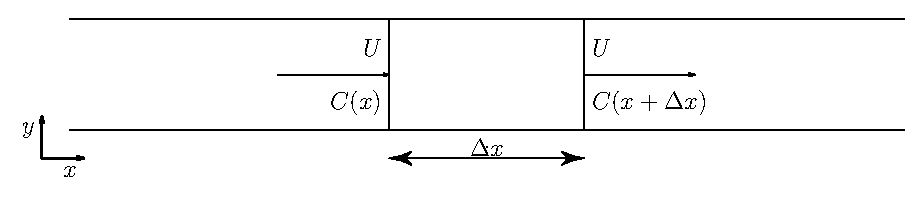
\includegraphics[width=\textwidth]{Figures/mass_transfer.eps}
\caption{The mass transfer in the moving liquid. \label{fig:moving:frame}}
\end{figure}

If one can assume that the mass point sources are distributed in the whole medium, then the mass accumulated in the unit volume $V=A \Delta x$ can be calculated as the difference of 
mass fluxes entering and leaving domain $U \bigl(C(x+\Delta x)-C(x)\bigr)$. We assume that the
source is a point source with the effective perimeter (area) $P$. The accumulated mass should be proportional
to the mass transfer coefficient:
\beq
U \bigl(C(x+\Delta x)-C(x)\bigr)=k_L P \bigl(\cstar-C(x)\bigr), 
\feq 
giving the same equation but only in the coordinate domain:
\beq
C(x)= \cstar \Bigl(1-\exp\bigl(-k_L a \frac{x}{U} \bigr)\Bigr).
\label{main:mass:transfer:expression} 
\feq

\item If one transfers to the frame moving with the liquid velocity $U$, then the situation will be
the same as in the first case. However, one can connect the time and spatial location with the
velocity $U$ ($t=\frac{x}{U}$) to obtain the same equation as in the case 2.
\end{enumerate}

\subsection{Bubble train}
In the application to the bubble train flow, if one can think of one bubble to be a point source,
then all considerations above are valid. For example, the expression
(\ref{main:mass:transfer:expression}) was used in the experiments by
\citet{bercic-mass}. However, one should be accurate with the definition of velocities because two
different phases co-exist in the bubble train flow. Usually, one can take the velocity $U$ to be as
a bulk velocity or $U=\ugas+\uliq$, where $\ugas$ and $\uliq$ are liquid and gas
superficial velocities correspondingly. 

Though the experimental measurements are straightforward as measuring concentrations at different
locations and calculating the volumetric mass transfer coefficient through the logarithmic
function. However, if one wants to analytically estimate the mass transfer coefficients, the
situation is much more complicated because of two phases presence and complicated bubble
geometry. Phases can have different mixing patterns
from film to slug and from slug to film. As it was mentioned before depending on the capillary
number the mixing velocity pattern is different. Analytical approaches
\cite{irandoust,vanbaten-circular} assume that the
contributions from film and bubble caps can be calculated separately. However, one can see that
such 
an assumption for bubble caps (slug well mixed and the concentration is uniformly distributed over
the slug) usually overpredicts the mass transfer \cite{irandoust}. This happens since some tracer
concentration from film is mixed with the slug and changes the overall concentration in the slug.
Thus, all estimations for the analytical mass as well do not account mutual mass transfer from
neighbouring bubbles.

Another issue is that if the slug is long enough then the film saturates with the tracer
concentration and its influence on the mass transfer can be negligible \cite{vanbaten-circular}.
Mixing patterns of the film and the liquid slugs are of great importance for the analytical
estimation of the mass transfer \cite{yue-mass}. However, the assumptions usually taken for the
mass transfer calculation are small capillary number and certain mixing patterns which help to
estimate the mass transfer using the penetration theory of \citet{higbie}.

The numerical approach can take into the account the complicated mixing patterns and geometries.
However, there is a  challenge to restore the continous approach as it is seen in experiments. Next
section gives more details about numerical simulations.
 
\subsection{Numerical simulations}
To restore the continuous picture one needs to perform a number of bubbles simulations. As we saw
before there are two approaches towards it - either to simulate
the bubble train and then to measure concentration along the pipe, Eq.
\ref{main:mass:transfer:expression}, or to transfer to the reference frame moving with the bulk
velocity $U$ and conduct same measurements. However, both methods do require a tracking of
moving bubbles which is complicated from the numerical point of view. Therefore, one needs to come
up with the simple smaller domain calculations of the mass transfer coefficient, which mimic the
continuous picture with infinite numbers of the bubbles closely. 

To avoid complications with moving grids, our
approach is to simulate mass transfer in the reference frame moving with the bubble. Therefore, one
needs to examine the equation for the continuous approach, Eq.
\ref{main:mass:transfer:expression}. 

We perform simulations in the frame moving with the bubble (velocity
$\ububble$), that the bubble position stands steady. The bubble velocity $\ububble$ is
different from the bulk velocity $\ugas+\uliq$. In this case we need to perform a coordinate $x$
variable change:
\beqal
\label{theor:average:concentration:time}
&x(t)=\ububble t\\
&C(x)=\cstar \Bigl(1-\exp\bigl(-\vol \frac{x}{\ugas+\uliq}\bigr)\Bigr)\\
&C(t)=\cstar \Bigl(1-\exp\bigl(-\vol\, t \frac{\ububble}{\ugas+\uliq}\bigr)\Bigr).
\feqal
Therefore, one can obtain the volumetric mass transfer coefficient through the concentration:
\beqal
&\vol\, t \frac{\ububble}{\ugas+\uliq}=\ln \frac{\cstar}{\cstar-C(t)}\\
&\volnondim=\frac{\lunit}{\ububble t}\ln \frac{\cstar}{\cstar-C(t)},
\feqal
where the parameter $\vol \frac{\lunit}{\ugas+\uliq}$ is non-dimensional. One can also measure the
volumetric mass transfer coefficient from concentrations given at times $t_1$ and $t_2$:
\beq
\label{theor:continuous:mass:transfer}
\volnondim=\frac{\lunit}{\ububble
(t_2-t_1)}\ln\frac{C^{*}-C(t_1)}{C^{*}-C(t_2)}.
\feq
Expressions (\ref{theor:average:concentration:time}) and (\ref{theor:continuous:mass:transfer}) are
the cornerstones of the present work. The main questions arisen in the present work are to define
$C(t)$ and  the boundary conditions to produce a proper volumetric mass transfer coefficient
$\vol$. 
  
Three possible scenarios of conducting numerical simulations are possible: 
\begin{enumerate}
\item As far as the hydrodynamic flow is periodic, one can make an assumption of the same boundary
conditions applied to the tracer concentration. Therefore, only one unit cell is simulated with
periodic boundary conditions, see Fig. \ref{fig:benchmark}. As well, no tracer leaves a
domain. The situation resembles a situation for the plug flow, where no tracer can leave a unit
domain. We expect such a situation happening for small Capillary numbers $Ca<0.1$, where the film
is thin and saturates fast with the tracer. Though easier to implement, it rises certain critisism
towards the inlet concentration to be equal to the outlet concentration. In the continuous
formulation there is the concentration difference between inlet and outlet involving the volumetric
mass transfer coefficient:
\beq
\volnondim=\ln\frac{\cstar-\cinlet}{\cstar-\coutlet}.
\feq
The concentration $C(t)$ required for calculation the volumetric mass transfer coefficient, Eq.
(\ref{theor:average:concentration:time}), can be taken as the average concentration in the domain:
\beq
\label{average:concentration:definition}
C(t)=\frac{\int_{liquid}{C \mathrm{d}V}}{\int{\mathrm{d}V}}.
\feq
\begin{figure}[htb!]
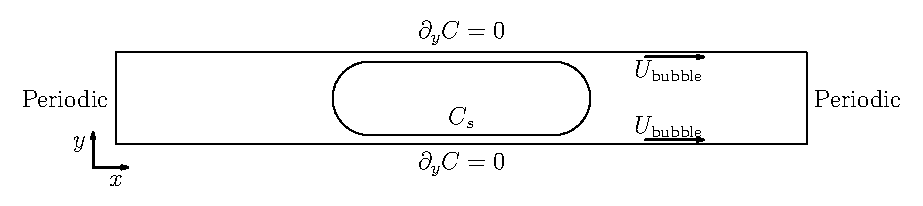
\includegraphics[width=\textwidth]{Figures/benchmark_middle.eps}\\
\caption{The two-dimensional benchmarks for the  the mass transfer
coefficient (bottom) for the bubble located near the entrance (top) and at the middle of the domain
(bottom). \label{fig:benchmark}}
\end{figure}
\item The second approach is the same as the first one but the concentration is taken as in
\cite{vanbaten-circular}. The characteristic concentration is taken as the inlet/outlet
concentration:
\beqal
&\cinlet=\frac{\int{U(y) C(0,y,t) \mathrm{d}y}}{\int{U(0,y) \mathrm{d}y}}\\
&\coutlet=\frac{\int{U(y) C(\lunit,y,t) \mathrm{d}y}}{\int{U(\lunit,y) \mathrm{d}y}}\\
&\cinlet=\coutlet.
\feqal
Therefore the assumptions  of this approach is that the difference between inlet and outlet is not
considerably large and the tracer is well mixed in the slug. 

\item
The approach of \citet{vanbaten-circular} is taken. Periodic boundary conditions were used. By the
definition the mass transfer coefficient is
proportional to the gain of the mass in the system divided by the concentration difference
multiplied on the surface area:
\beq
\vol=\frac{\dot{m}}{P \Delta C}\frac{P}{V}=\frac{\dot{m}}{V (\cstar-C(t))},
\feq
where mass difference in the domain can be calculated as:
\beq
\dot{m}=\frac{m_2-m_1}{t_2-t_1}=\frac{\int_{liq}{C(t_2)\mathrm{d}V}-\int_liq{C(t_1)\mathrm{d}V}}{
t_2-t_1 } .
\feq
In the approach of \citet{vanbaten-circular} the inlet and outlet concentrations were taken as the
characteristic concentration $C(t)$.

\item 
The approach of the opened boundaries was examined, see Fig. \ref{fig:benchmark:jos}. At the inlet
and outlet boundaries the diffusion flux was imposed to be zero, $\frac{\partial C}{\partial x}=0$.
The characteristic concentration was taken as the average concentration in the whole domain.
\begin{figure}
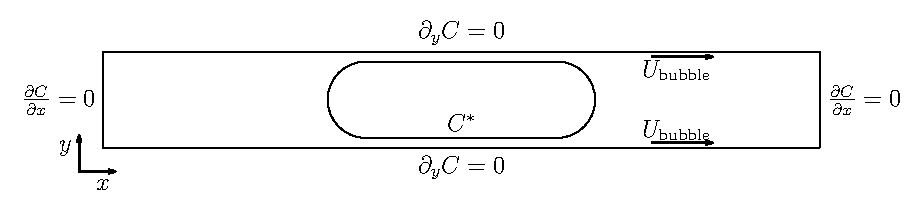
\includegraphics[width=\textwidth]{Figures/benchmark_jos.eps}
\caption{The numerical mass transfer benchmark with open boundaries. The mass transfer is
calculated according to Eq. \ref{theor:average:concentration:time} with the characteristic
concentration accoring to Eq. \ref{average:concentration:definition}. \label{fig:benchmark:jos}}
\end{figure}

\item 
The last approach to be examined in this paper is the approach of the simulation of a lot of unit
volumes, see Fig. \ref{big:benchmar:alot}. This situation corresponds to the simulation of the
bubble train head, after injecting to the pipe and travelling along the pipe. The argument here is
that behind a certain number of the bubble train head, the influence of the boundaries will be
diminished. Thus, the average concentration in time will be governed by Eq.
\ref{theor:continuous:mass:transfer}. This simulation statement is of most correspondence to
experiments and should give right answer. However, one of the
disadvantages is to simulate a certain number of unit cells, thus increasing a computational
complexity.
\begin{figure}[htb!]
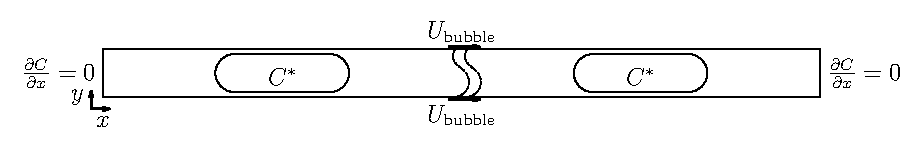
\includegraphics[width=\textwidth]{Figures/benchmark_alot.eps}\\
\caption{Benchmark for a lot of units. \label{fig:benchmark:alot}}
\end{figure}
\end{enumerate} 

Before all the approaches will be examined we will perform benchmarks of parts of geometries that
form a problem.

\section{Validation}
As for analytical expressions the problem of the mass transfer can be decomposed to the following
parts: the mass transfer from two hemispheres and the mass transfer from the film. We will examine
these problems with the help of the lattice Boltzmann method and compare them against analytical
solutions. The next sections will present the lattice Boltzmann method and a few benchmarks.

\subsection{TRT $D2Q9$ model}
The lattice Boltzmann equation (LBE) operates on a rectangular grid representing the
physical domain. It utilizes
probability distribution functions (also known as particle populations)
containing information about
macroscopic variables, such as fluid density and momentum. LBE consists of
two parts: a local collision step, and a propagation step which transports
information from one node to another along some 
directions specified by the discrete velocity set.
The LBE is typically implemented as follows:
\begin{equation}
\label{standard:implementation}
\begin{aligned}
&f_i^{*}(\bm{x},t)= f_i(\bm{x},t)-\omega \bigl(f_i(\bm{x},t)-f_i^{eq}(\bm{x},t)\bigr),&&\text{
collision step}\\
&f_i(\bm{x}+\bm{c_i},t+1)=f_i^{*}(\bm{x},t),&&\text{ propagation step}, 
\end{aligned}
\end{equation}
where $f_i$ is the probability distribution function in the direction $\bm{c_i}$,
 $f_i^{eq}$ is the equilibrium probability distribution function, $\omega$ is the
relaxation parameter. Collision operator, $-\omega \bigl(f_i- f_i^{eq}\bigr)$ is so-called BGK
collision operator \cite{bgk}. However, the approach to be used here is the TRT
(two-relaxation-times) collision operator \cite{ginzburg-main,ginzburg-saturated-flow}. In
comparison with the widely used BGK collision operator, TRT collision operator have better accuracy
for diffusion and convection fluxes, larger range of parameters where the LBM scheme is stable.

The TRT collision operator \cite{ginzburg-boundary-main}
decomposes the populations and the equilibrium
distribution into the symmetric and antisymmetric parts:
\begin{equation}
\label{trtdecomp}
f^{\pm}_i=\frac{f_i\pm f_{\bar{i}}}{2}\;,\; 
{eq_i}^{\pm}=\frac{eq_i\pm eq_{\bar{i}}}{2}\;,
\end{equation}
where $\bar{i}$ is the opposite direction to the $i$-th direction.
The collision is performed with two independent relaxation rates for 
symmetric and antisymmetric modes:
\begin{equation}
\label{trt}
\begin{aligned}
&f_i^{*}(\bm{x},t)=f_i(\bm{x},t)-\omegaplus (f_i^{+} - eq_i^+)-\omegaminus
(f_i^{-} -
eq_i^-)\\
&f_i(\bm{x}+\bm{c_i},t+1)=f_i^{*}(\bm{x},t).
\end{aligned}
\end{equation}
Note that the BGK collision operator is the particular subclass of the TRT relaxation operator with
$\omegaplus=\omegaminus$. In comparison with the BGK collision operator,
the TRT collision operator has the additional degree of freedom. Thus, the TRT operator then
introduces
so-called magic (free) parameter
$\Lambda=\Bigl(\frac{1}{\omegaplus}-\frac{1}{2}\Bigr)\Bigl(\frac{1}{\omegaminus}-\frac{1}{2}
\Bigr)$. 
This free parameter controls the effective location of the bounce-back
walls \cite{ginzburg-multireflection}, second-order accuracy of
boundary \cite{ginzburg-boundary-main} and interface schemes \cite{ginzburg-discontinious}, 
spatial accuracy \cite{ginzburg-recurrence,servan-trt-stability},
consistency \cite{ginzburg-brinkman} and, to some extent,
stability \cite{kuzmin-stability-optimal,kuzmin-d1q3,servan-trt-stability}.
In particular, $\Lambda=\frac{1}{4}$ achieves the optimal stability for the
linear advection-diffusion isotropic equation \cite{kuzmin-stability-optimal}. 

The parameters $\omegaplus$, $\omegaminus$ and $f_i^{eq}$ fully define the lattice Boltzmann
procedure. The two-dimensional nine velocities LBM $D2Q9$ is defined on the set of lattice
velocities with coordinates:
\beqal
&c_{ix}=\{0,1,0,-1,0,1,-1,-1,1\},\text{ for } i=0\dots8\\
&c_{iy}=\{0,0,1,0,-1,1,1,-1,-1\},\text{ for } i=0\dots8\,.
\feqal

The equilibrium functions for $D2Q9$ TRT model are represented as \cite{kuzmin-stability-optimal}:
\begin{equation}
\begin{aligned}
&eq_i^{+}=eq_i^{(m)}+g^{(u)} eq_i^{(u)}\\
&eq_i^{(m)}=t_i^{(m)} c_e+ eq_i^{(a)}\\
&eq_i^{(u)}=t_i^{(u)} \frac{u_x^2+u_y^2}{2}+\frac{u_x^2-u_y^2}{4} p_i^{(xx)}+g_{xy}^{(u)}\frac{u_x
u_y}{4} p_i^{xy}\\
&eq_i^{(a)}=\frac{D_{xx}-D_{yy}}{4} p_i^{xx}+\frac{D_{xy}}{4} p_i^{(xy)},
\end{aligned}
\end{equation}
where $D_{xx,yy,xy}$ are components of the diffusion tensor, $c_e=\frac{D_{xx}+D_{yy}}{2}$, the tensor $p_i^{(xx)}=c_{ix}^2-c_{iy}^2$, the tensor  $p_i^{(xy)}=c_{ix} c_{iy}$, the weights
$t_i^{(u,m,a)}$ can be chosen based on stability criteria. Though not the best set of weights for
stability, but the most spread set of weights, so called ``hydrodynamic`` weights, was chosen:
\begin{equation}
t_i^{(u)}=t_i^{(m)}=t_i^{(a)}=\Bigl\{0,\frac{1}{3},\frac{1}{3},\frac{1}{3},\frac{1}{3},\frac{1}{12},
\frac {1}{12},\frac{1}{12},\frac{1}{12}\Bigr\}
\end{equation}
 
It can be shown through the Chapman-Enskog procedure \cite{chapman}, that the simple update rule
with the equilibrium function presented above restores the anisotropic
advection-diffusion equation:
\beq
\partial_t C+ \partial_{\alpha} C u_{\alpha}=\partial_{\alpha\beta} K_{\alpha\beta} C,
\feq
where $K_{\alpha\beta}=\Bigl(\frac{1}{\omegaminus}-\frac{1}{2}\Bigr)D_{\alpha\beta}$
with the
following diffusion tensor:
\begin{equation}
D_{\alpha\beta}=
\begin{pmatrix}
D_{xx} + (g^{(u)}-1) u_x^2 & D_{xy}+(g_{xy}^{(u)}-1)u_x u_y\\
D_{xy} + (g_{xy}^{(u)}-1) u_x u_y& D_{yy}+(g^{(u)}-1) u_y^2 
\end{pmatrix}
\end{equation}
We want to resolve the isotropic advection-diffusion equation, $D=D_{xx}=D_{yy}$ or $K=K_{xx}=K_{yy}$, with the non-diagonal diffusion tensor components to be zero $D_{xy}=0$. In comparison with the $D2Q5$ model, with the $D2Q9$ it is
possible to cancel the numerical diffusion by the proper choice
of the equilibrium functions, i.e. $g_{xy}^{(u)}=g^{(u)}=1$.  The particular choice of parameters used in simulations is $c_e=\frac{1}{3}$, $\Lambda=\frac{1}{4}$. Thus, the diffusion coefficient $K$ is matched through $\omegaminus$, i.e. $K=c_e \Bigl(\frac{1}{\omegaminus}-\frac{1}{2}\Bigr)=\frac{1}{3}(\frac{1}{\omegaminus}-\frac{1}{2}\Bigr)$. From hereon, without a loss of generality we refer to diffusion coefficient 
$K$ as $D$.  Free relaxation parameter $\omegaplus$ can be found through $\Lambda$. For particular choice $\Lambda=\frac{1}{4}$ (the optimal stability parameter), $\omegaplus$ can be found easily as $\omegaplus=2-\omegaminus$.  Fig. \ref{stability:d2q9} shows the stability limits for the $D2Q9$ model $c_e$ against $U^2=u_x^2+u_y^2$ for two particular choices.
\begin{figure}[htb!]
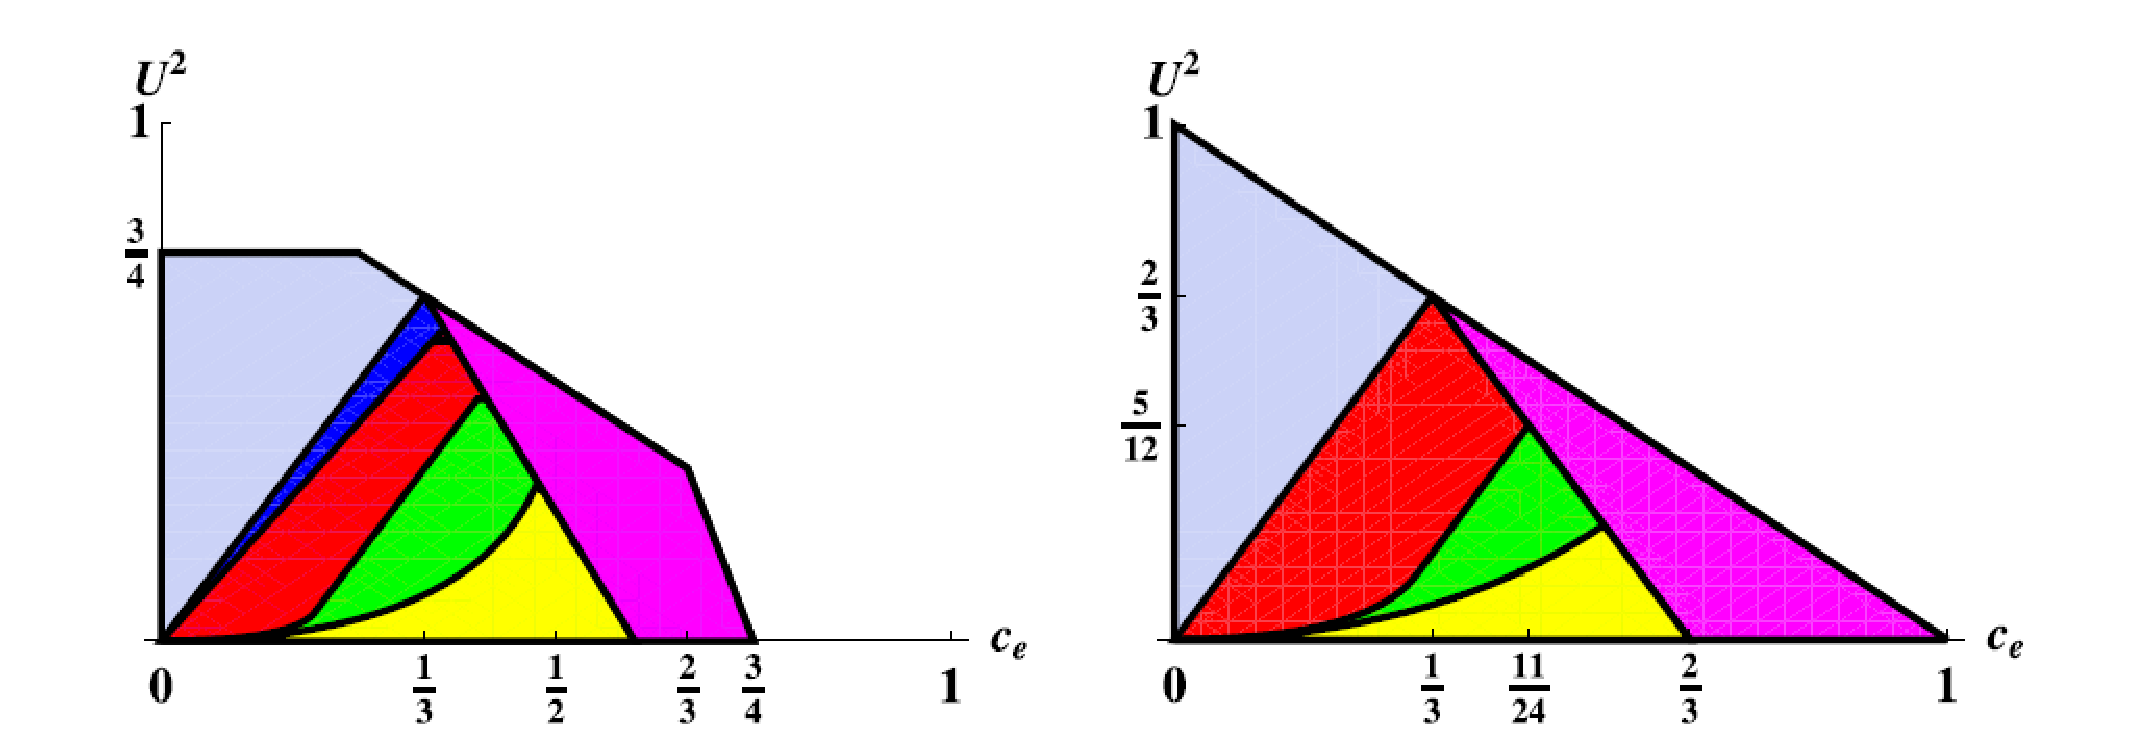
\includegraphics[width=\textwidth]{Figures/d2q9_stability.eps}
\caption{The stable sub-domains of the $D2Q9$ schemes ($\Lambda=\frac{1}{4}$)
are plotted for standard (hydrodynamic) weights (left) and uniform weights (right, not mentioned here) when the
numerical diffusion is removed, partially or completely. For particular choice used in this work (hydrodynamic weights, $c_e=\frac{1}{3}$, left picture), the achieved stable velocity is $u_x^2+u_y^2\leq\frac{2}{3}$. The non-negativity of populations (green+yellow) is for BGK stability. One can see that the achieved maximum stable velocity is twice smaller $u_x^2+u_y^2\leq \frac{1}{3}$ for the BGK collision operator.The proper choice of weights can
allow to obtain  total triangle $0 \leq u_x^2+u_y^2 \leq 1- c_e$ (the
uniform weights only).
\label{stability:d2q9}}
\end{figure}
{\color{red} Here need to cover boundary conditions}

Note that the parameters of the lattice
Boltzmann are connected with the physical parameters only through the non-dimensional
numbers governing the physics of the problem. In our case, this number is the Peclet number, $Pe=\frac{\ububble L}{D}$.
Therefore, one can substitute any quantity, i.e.
$\ububble$ in the lattice Boltzmann units as soon as the
Peclet number is the matched in physical space and numerical simulations. This fact that $\ububble$ can be chosen arbitrarily is extremely useful in the context of numerical simulations, since can increase the time step, or decrease the computational demand by order of magnitude to obtain meaningful results. This point will be extensively covered later. 

Next section will cover LBM benchmarks for problems that form the mass transfer problem, as mass transfer from the film  and hemispheres.

\subsection{The radial case}
The case to be examined here is the mass transfer from the stair-case boundary which represents a circle. It can be
prescribed by the following system of equations:
\beq
\begin{aligned}
&\partial_t C(r,t)=\frac{1}{r}\partial_r r \partial_r C(r,t)\\
&C(a,t)=C_0,\,C(r,0)=C_{init}
\end{aligned}
\feq 
The solution is represented as \cite{chemical-correlations}:
\beq
\frac{C(r,t)-C_{0}}{C_{init}-C_{0})}=\sum_{n=1}^{\infty}{\frac{2}{\mu_n
J_1(\mu_n)}\exp\Bigl(-\mu_n^2 \frac{D t}{a^2} \Bigr)J_0(\mu_n \frac{r}{a})},
\feq
where $\mu_n$ is the $n$-th zero root of the $0$th order Bessel polynomial $J_0(\mu_n)=0$. Some of
the corresponding roots are as follows: $\mu_1=2.4048$,$\mu_2=5.5201$,$\mu_3=8.6537$,
$\mu_4=11.7915$,$\mu_5=14.9309$.
By taking initial concentration to be $0$, one can obtain the following solution:
\beq
C(r,t)=C_0 \Biggl(1 - \sum_{n=1}^{\infty}{\frac{2}{\mu_n
J_1(\mu_n)}\exp\Bigl(-\mu_n^2 \frac{D t}{a^2} \Bigr)J_0(\mu_n \frac{r}{a})}\Biggr).
\feq

The solution depends only on the non-dimensional time: $\tau=\frac{D t}{a^2}$. The domain size was $129\times 129$ with the circle radius $a=40$ units. Some examples for
different diffusion coefficients are presented in Fig.\ref{fig:cylinder:benchmark}.
\begin{figure}[htb!]
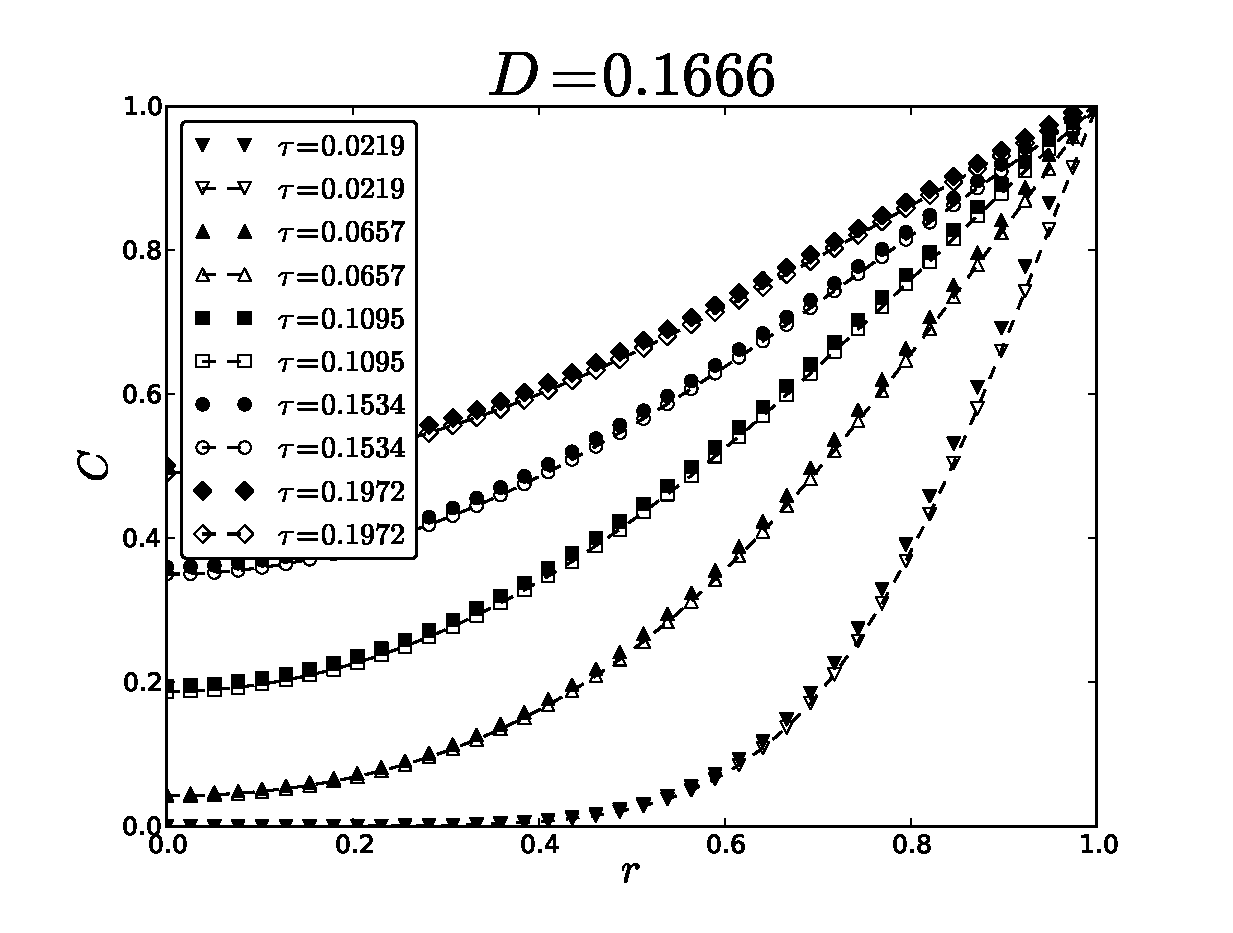
\includegraphics[width=0.5\textwidth]{Figures/cylinder1666.eps}
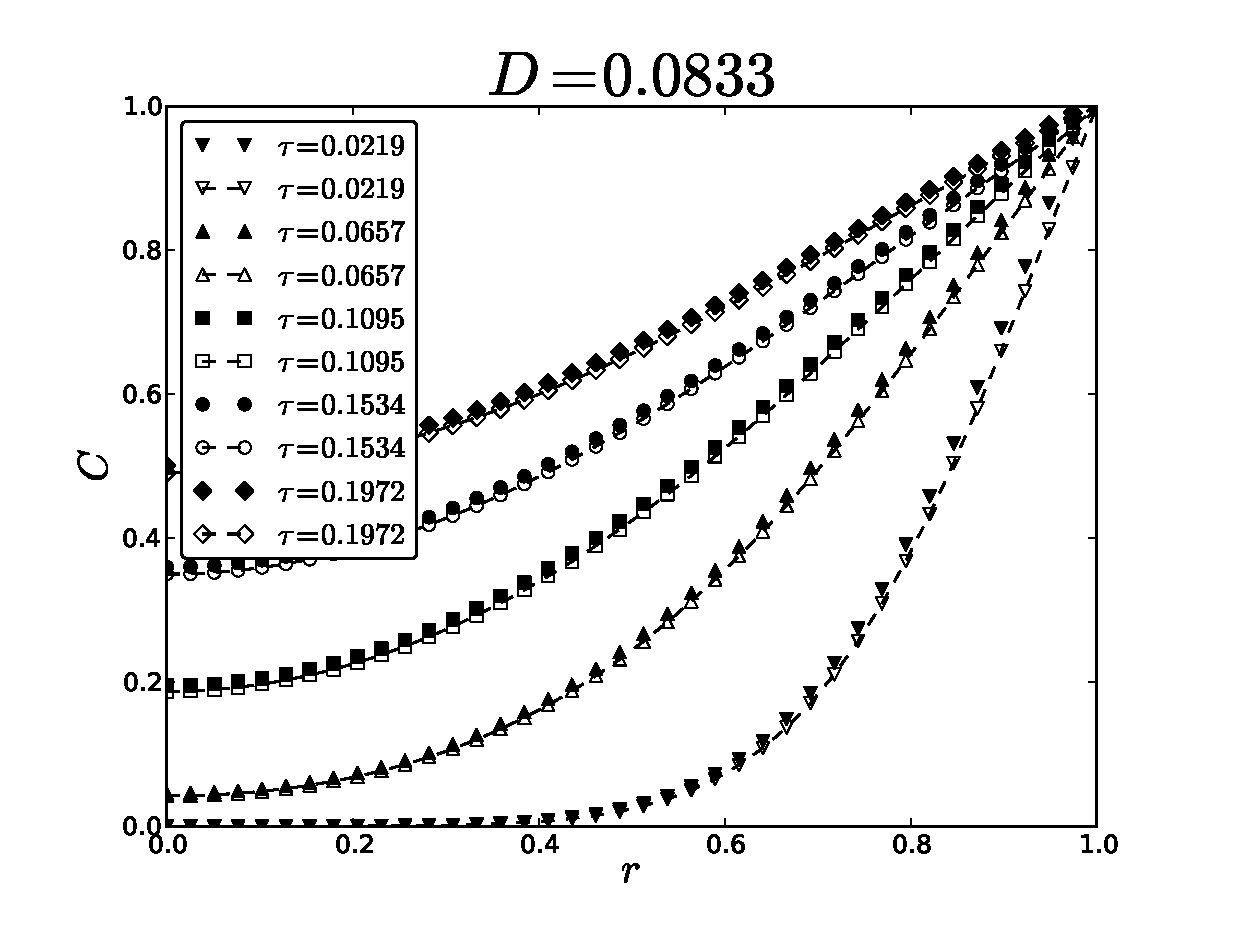
\includegraphics[width=0.5\textwidth]{Figures/cylinder0833.eps}\\
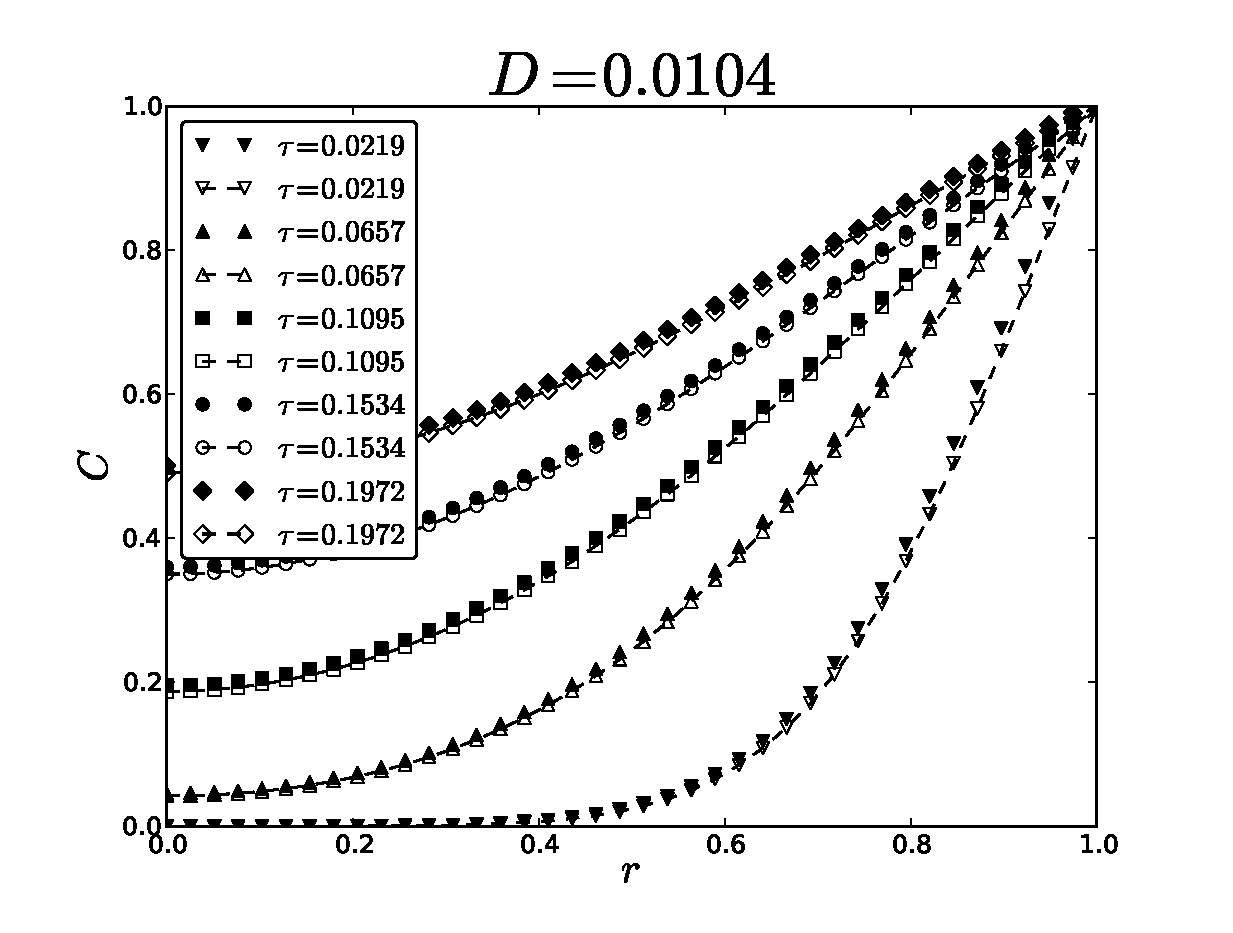
\includegraphics[width=0.5\textwidth]{Figures/cylinder0104.eps}
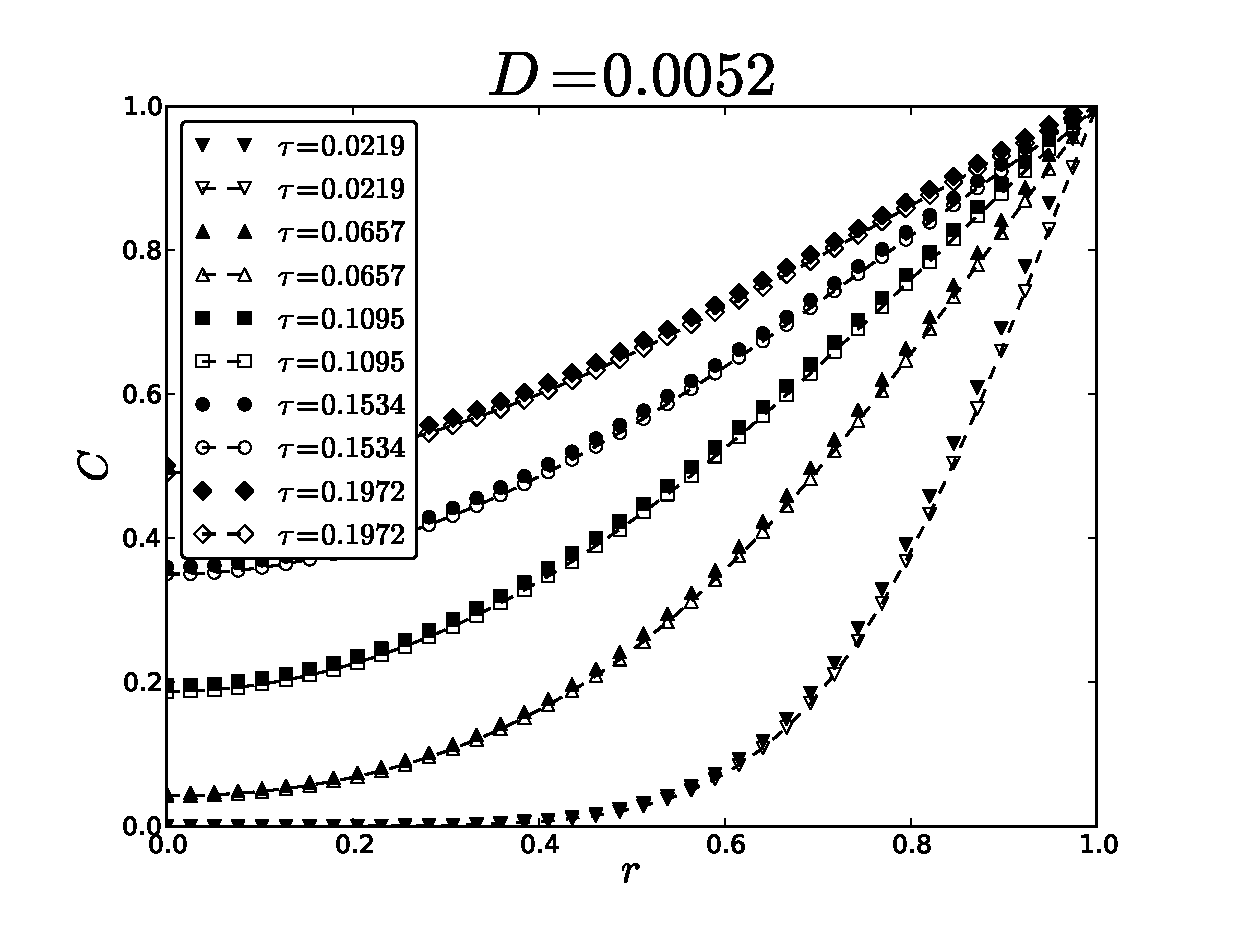
\includegraphics[width=0.5\textwidth]{Figures/cylinder0052.eps}\\
\caption{Profiles for different diffusion parameters varied with $\omegaminus$. One can see that the diffusion from the non-linear boundaries is captured
accurately \label{fig:cylinder:benchmark}.}
\end{figure}

\subsection{Parabolic profile with velocity zero gradient at the wall}
The problem is defined in terms of PDE as follows: 
\beq
\begin{aligned}
&\frac{\partial C}{\partial x} U(y)=D\frac{\partial^2 C}{\partial y^2}\\
&C(0,y)=C_0,\, C(x,0)=C_{wall},\, \frac{\partial C}{\partial y }(x,\delta)=0\\
&U(y)=U_0 \Bigl(\frac{y}{\delta}\Bigr)^2
\end{aligned}
\feq
The system after non-dimensionalization becomes as follows:
\beq
\begin{aligned}
&\frac{\partial C}{\partial \frac{x}{H}} \frac{U_0}{H}
\Bigl(\frac{y}{H}\Bigr)^2=\frac{D}{H^2}\frac{\partial^2 C}{\partial \frac{y^2}{H^2}}\\
&C(0,y)=C_0,\, C(x,0)=C_{wall},\, \frac{\partial C}{\partial y }(x,H)=0\\
\end{aligned}
\feq
After a change of variables:
\beq
\begin{aligned}
&\zeta=\frac{x}{H} \frac{D}{U_0 H}=\frac{1}{Pe}\frac{x}{H}\\
&\xi=\frac{y}{H}
\end{aligned}
\feq
, the equation with boundary conditions becomes as follows:
\beq
\begin{aligned}
&\frac{\partial C}{\partial \zeta}\xi^2=\frac{\partial^2 C}{\partial \xi^2}\\
&C(0,\xi)=C_0\\
&C(\zeta,0)=C_{wall}\\
&\frac{\partial C}{\partial \xi}(\zeta,1)=0\\
\end{aligned}
\feq 
Still the equation cannot be solved with the separation of variables as it requires the homogenuos
boundary conditions. Thus, let us introduce the new variable to be $\Theta=C-C_{wall}$. The system
will be changed but not considerably:
\beq
\begin{aligned}
&\frac{\partial \Theta}{\partial \zeta}=\frac{1}{\xi^2}\frac{\partial^2 \Theta}{\partial \xi^2}\\
&\Theta(0,\xi)=C_0-C_{wall}\\
&\Theta(\zeta,0)=0,\, \partial_{\xi}\Theta(\zeta,1)=0\\
\end{aligned}
\feq 
This equation can be solved by separation of variables if the solutions is represented as the
multiplication of two functions $\Theta(\zeta,\xi)=X(\zeta)Y(\xi)$. The differential equation will
become as follows:
\beq
\begin{aligned}
&\frac{\mathrm{d} X(\zeta)}{\mathrm{d} \zeta}Y(\xi)=\frac{X(\zeta)}{\xi^2}\frac{\mathrm{d^2}
Y(\xi)}{\mathrm{d}\xi^2}\\
&\frac{1}{X(\zeta)}\frac{\mathrm{d} X(\zeta)}{\mathrm{d} \zeta}=\frac{1}{\xi^{2} Y(\xi)}
\frac{\mathrm{d^2} Y(\xi)}{\mathrm{d}\xi^2}
\end{aligned}
\feq
The left and right parts depend on different variables. Therefore to be equal to each other both
parts equal to constant, say $-m^4$. Thus, the separation of the variables leads to two ODE
equations:
\begin{equation*}
\begin{aligned}
&\frac{\mathrm{d}X(\zeta)}{\mathrm{d}\zeta}=-m^4 X(\zeta)\\
&\frac{\mathrm{d^2}Y(\xi)}{\mathrm{d}\xi^2}+m^4 \xi^2 Y(\xi)=0\\ 
\end{aligned}
\end{equation*}
The solution of the first equation is the exponential function:
\beq
X(\zeta)=\exp(-m^4 \zeta)\\
\feq
The solutions of the second equation are two hypergeometric function which can be expressed through
the Bessel functions \cite{abramowitz}:
\beq
\begin{aligned}
&Y_1=\sqrt{\xi}J_{\frac{1}{4}}\Bigl(\frac{m^2 \xi^2}{2}\Bigr)\\
&Y_2=\sqrt{\xi}J_{-\frac{1}{4}}\Bigl(\frac{m^2 \xi^2}{2}\Bigr)\\
&Y'_1=m^2 \xi^{3/2} J_{-\frac{3}{4}}\Bigl(\frac{m^2 \xi^2}{2}\Bigr)\\
&Y'_2=m^2 \xi^{3/2} J_{\frac{3}{4}}\Bigl(\frac{m^2 \xi^2}{2}\Bigr)\\
\end{aligned}
\feq
The solution is the summation of two functions:
\begin{equation*}
Y(x)=C_1 Y_1(x)+C_2 Y_2(x). 
\end{equation*}
One can find coefficients from the boundary conditions:
\beq
\begin{aligned}
&Y(0)=0=C_1 Y_1(0)+C_2 Y_2(0)\\
&Y_1(0)=0,\,Y_2(0)=\frac{\sqrt{2}}{\sqrt{m} \Gamma(3/4)}\, C_2=0\\
&Y'(1)=0=C_1 Y'_1(1)+C_2 Y'_2(1)=C_1 Y'_1(1)\\
&J_{-\frac{3}{4}}\Bigl(\frac{m^2}{2}\Bigr)=0
\end{aligned}
\feq
Therefore one needs to find zeros of $J_{-\frac{3}{4}}\Bigl(\frac{m^2}{2}\Bigr)$. To give some
numerical values:
$m_1=1.454997085$, $m_2=2.927133004$, $m_3=3.857578101$, $m_4=4.601777732$, $m_5=5.240824067$.
Therefore a solution in a general form is represented as:
\beq
\Theta(\zeta,\xi)=\sum_m{C_m \sqrt{\xi} J_{\frac{1}{4}}\Bigl(\frac{m^2
\xi^2}{2}\Bigr)\exp(-m^4 \zeta)}
\feq
To find unknown coefficients $C_m$ one needs to substitute the expression above to the initial
condition:
\beq
\Theta(0,\xi)=C_0-C_{wall}=\sum_m{C_m \sqrt{\xi}J_{\frac{1}{4}}\Bigl(\frac{m^2
\xi^2}{2}\Bigr)}\\
\feq
Using the Stourm-Liouville theorem one can multiply by $\xi^{5/2}
J_{\frac{1}{4}}\Bigl(\frac{m^2 \xi^2}{2}\Bigr)$ and integrate left and right parts of the equation:
\beq
\begin{aligned}
&\bigl(C_0-C_{wall}\bigr) \int_{\xi=0}^{1}{\xi^{5/2} J_{\frac{1}{4}}\Bigl(\frac{m^2
\xi^2}{2}\Bigr)\mathrm{d}\xi}=C_m\int_{\xi=0}^{1}{\xi^3 J_{\frac{1}{4}}^2\Bigl(\frac{m^2
\xi^2}{2}\Bigr)\mathrm{d}\xi}\\
&C_m = (C_0-C_{wall}) \frac{\int_{\xi=0}^{1}{\xi^{5/2} J_{\frac{1}{4}}\Bigl(\frac{m^2
\xi^2}{2}\Bigr)\mathrm{d}\xi}}{\int_{\xi=0}^{1}{\xi^3 J_{\frac{1}{4}}^2\Bigl(\frac{m^2
\xi^2}{2}\Bigr)\mathrm{d}\xi}}
\end{aligned}
\feq
Therefore, the overall solution is specified as:
\beq
\begin{aligned}
&C(x,y)=C_{wall}+\sum_{m}{C_m
\sqrt{\frac{y}{H}}J_{\frac{1}{4}}\Bigl(\frac{m^2}{2}\frac{y^2}{H^2}\Bigr)\exp\Bigl(-\frac{m^4}{Pe}
\frac { x }{H}\Bigr)}\\
&C_m = (C_0-C_{wall}) \frac{\int_{\xi=0}^{1}{\xi^{5/2} J_{\frac{1}{4}}\Bigl(\frac{m^2
\xi^2}{2}\Bigr)\mathrm{d}\xi}}{\int_{\xi=0}^{1}{\xi^3 J_{\frac{1}{4}}^2\Bigl(\frac{m^2
\xi^2}{2}\Bigr)\mathrm{d}\xi}}
\end{aligned}
\feq

\subsection{The parabolic profile mass transfer and comparison}
The problem we want to address can be formulated through the following PDE:
\beq
\begin{aligned}
&\frac{\partial C}{\partial x} U(y)=D\frac{\partial^2 C}{\partial y^2}\\
&C(0,y)=0,\, C(x,\pm \delta)=C_s,\, \frac{\partial C}{\partial y }(x,0)=0\\
&U(y)=U_0 \Bigl(1-\bigl(\frac{y}{\delta}\bigr)^2\Bigr)
\end{aligned}
\feq
The same procedure can be done as in the previous case to redefine variables. After substitution
the following can be obtained:
\beq
\begin{aligned}
&\frac{\partial \Theta}{\partial \zeta}(1-\xi^2)=\frac{\partial^2 C}{\partial \xi^2}\\
\Theta(\zeta,\xi)=C-C_s\,\Theta(0,\xi)=-C_s\,\Theta(0,\pm 1)=0\\
\end{aligned}
\feq
After separation of variables, $\Theta(\zeta,\xi)=X(\zeta)Y(\xi)$ one can come up with two
equations:
\beq
\label{fourier:separation:variables}
\begin{aligned}
&\frac{\mathrm{d}X(\zeta)}{\mathrm{d}\zeta}+m^4 X(\zeta)=0\\
&\frac{\mathrm{d^2}Y(\xi)}{\mathrm{d}\xi^2}+m^4 (1-\xi^2) Y(\xi)=0
\end{aligned}
\feq
The first equation has a solution:
\beq
X(\zeta)=\exp(-m^4 \zeta)
\feq
The second equation can be simplified after substitution $\bar{\xi}=m \sqrt{2} \xi$ to the standard
equation:
\beq
Y''-\Bigl(\frac{1}{4}\xi^2+a\Bigr)Y=0.
\feq
The equation above has two solutions via parabolic cylinder functions or through the confluent
hypergeometric function \cite{abramowitz}:
\beq
\begin{aligned}
&Y_1=e^{-x^2/4} {_1F_1}\Bigl(\frac{a}{2}+\frac{1}{4},\frac{1}{2},\frac{x^2}{2}\Bigr)\\
&Y_2=e^{-x^2/4} {_1F_1}\Bigl(\frac{a}{2}+\frac{3}{4},\frac{3}{2},\frac{x^2}{2}\Bigr)\\
\end{aligned}
\feq 
Taking symmetry conditions in the consideration by leaving only even solution, Eq.
(\ref{fourier:separation:variables}) has a solution as:
\beq
Y_m=C_m e^{-m^2 x^2/2} {_1F_1}\Bigl(-\frac{m^2}{4}+\frac{1}{4},\frac{1}{2},m^2 x^2\Bigr) 
\feq
To satisfy boundary condition we need to find zeros of the hypergeometric function, i.e.
${_1F_1}\Bigl(-\frac{m^2}{4}+\frac{1}{4},\frac{1}{2},m^2 \Bigr)=0$. First ten eigenvalues can be
found using numerical methods, as $1.2967$, $2.3811$,$3.1093$,$3.6969$,$4.2032$,$4.6548$,$5.0662$,
$5.4467$, $5.8023$,$6.1373$. One needs to satisfy one more condition to obtain coefficients $C_m$:
\beq
-C_{s}=\sum_m{C_m e^{-m^2 x^2/2} {_1F_1}\Bigl(-\frac{m^2}{4}+\frac{1}{4},\frac{1}{2},m^2
x^2\Bigr)} 
\feq
One can multiply both parts on $(1-x^2){_1F_1}\Bigl(-\frac{m^2}{4}+\frac{1}{4},\frac{1}{2},m^2
x^2\Bigr)$ and through orthoganality Sturm-Liouiville theorem obtain coefficients:
\beq
\label{coeff:series:parabolic:profile}
C_m=-C_s \frac{\int_{x=0}^{1}{(1-x^2)e^{-m^2 x^2/2}
{_1F_1}\Bigl(-\frac{m^2}{4}+\frac{1}{4},\frac{1}{2},m^2
x^2\Bigr)\mathrm{d}x}}{\int_{x=0}^{1}{(1-x^2)e^{-m^2 x^2/2}
{_1F_1}\Bigl(-\frac{m^2}{4}+\frac{1}{4},\frac{1}{2},m^2
x^2\Bigr)^2\mathrm{d}x}}
\feq
Therefore a whole solution can be written as:
\begin{equation}
C=C_{s}-C_s \sum_{m=0}{C_m e^{-m^4 \frac{x}{\delta}\frac{1}{Pe}} e^{-m^2
y^2/(2\delta^2)}{_1F_1}\Bigl(-\frac{m^2}{4}+\frac{1}{4},\frac{1}{2},m^2 \frac{y^2}{\delta^2}\Bigr)},
\end{equation}
where coefficients $C_m$ are taken from Eq. (\ref{coeff:series:parabolic:profile}). The comparison
between profiles is represented in Fig. \ref{fig:parabolic:comparison}.
\begin{figure}[htb!]
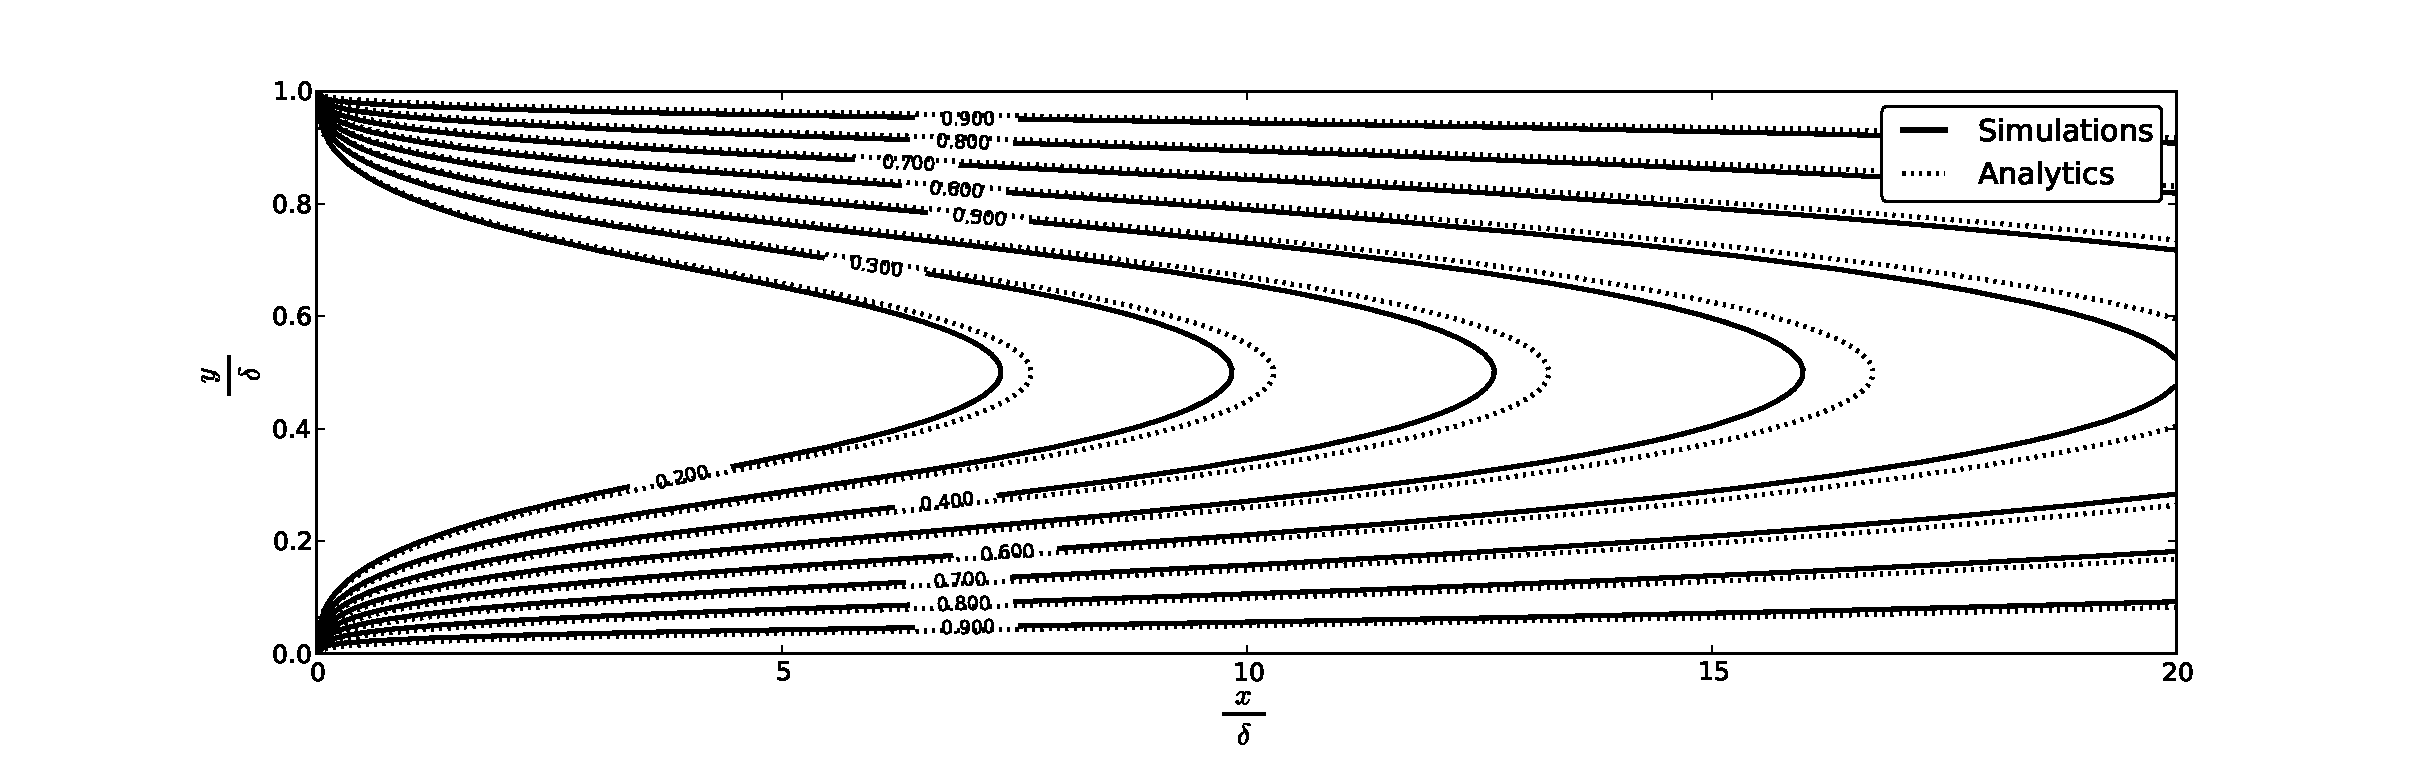
\includegraphics[width=\textwidth]{Figures/parabolic_profile_comparison.eps}
\caption{Comparison between analytical profile and simulations with pressure antibounceback
conditions. One can see given a low resolution of the profile a nice coincedence.}
\end{figure}

\section{Numerical approach}
\label{sec:numerics}
The numerical  procedure of studying mass transfer is presented in the following steps:
\begin{description}
 \item[Flow field] The hydrodynamics for the bubble motion in the periodic domain is obtained
according to the work \cite{kuzmin-binary2d}. The grid resolution is taken to insure grid
independency of results.  
 \item[Bubble reference frame] Once the hydrodynamics is resolved, the mass transfer simulations
are conducted in the moving
reference frame with the bubble. Then the bubble stands still and the flow is coming around the
bubble. We impose a steady concentration of solutant on the surface of the bubble.
\item[Mass transfer] One needs not only perform a Galilean transformation to the reference
frame moving with the bubble but also to
transfer the bubble to the inlet condition. This can insure that the studied phenomenon is a liquid
slug. 
\end{description}






\section{Mass transfer}
The mass transfer is characterized by non-dimensional numbers as Schmidt number (viscous diffusion
rate over mass diffusion rate), the Peclet number (convection over diffusion) and the Sherwood
number (convection mass transfer over diffusion mass transfer):
\begin{equation}
\begin{aligned}
&Pe=\frac{U L}{D}\\
&Sh=\frac{K L}{D}\\
&Sc=\frac{\nu}{D}\\
\end{aligned}
\end{equation}

As far as the lattice Boltzmann method operates only in the non-dimensional space, one needs to
match the non-dimensional lattice Boltzmann parameters with non-dimensional physical parameters.
Therefore, one needs to form non-dimensional numbers from the physical parameters. One of the
particular experiment examples is the
work by \citet{bercic-mass} who used the methane dissolution to characterize the mass transfer for
bubble train flow. 

In what follows we will perform the matching of obtained hydrodynamics results
\cite{kuzmin-binary2d} with physical ones from experiment of \citet{bercic-mass}. The diffusion
coefficient of the methane under standard conditions \cite{methane-properties} is
$1.84\times 10^{-5} \mathrm{cm}^2/\mathrm{s}$. The diameters of capillaries in the experiment were
as $1.5$, $2.5$ and
$3.1\,\mathrm{mm}$. For simplicity reasons we will choose the diameter of capillary as $1.5\,
\mathrm{mm}$. 
The non-dimensional parameters obtained from the hydrodynamics lattice Boltzmann simulations are
as:
\begin{equation}
\begin{aligned}
&Ca=\frac{U \mu_{\mathrm{liq}}}{\gamma}\\
&Re=\frac{\rho_{\mathrm{liq}} U L}{\mu_{\mathrm{liq}}}.
\end{aligned}
\end{equation}
Given some physical characteristics as the liquid density and the channel length,
one can obtain the physical velocity obtained from non-dimensional numbers:
\begin{equation}
\begin{aligned}
Ca\cdot Re= \frac{\rho_{\mathrm{liq}} U^2 L}{\gamma}\\
U=\sqrt{\frac{Ca\,Re\,\gamma}{\rho_{\mathrm{liq}}L}}
\end{aligned}
\end{equation}

Assuming that the surface tension of water is $0.0728\,\mathrm{N/m}$ (methane exhibits the same
trend \cite{schmidt-methane}), the density is       
$1000\,\mathrm{kg/m^3}$, the hydraulic diameter of the channel to be $1.5\,\mathrm{mm}$ one can
calculate the physical velocity of the bubble.
Table \ref{table:twod:simulations} represents lattice Boltzmann simulations results and their
physical equivalents for the grid $202\times 3002$. One can see
that velocity is quite reasonable
as \citet{bercic-mass} declared that experiments were conducted for velocities in the ranges of
$0.01$ to $0.4\,\mathrm{m}/\mathrm{s}$. 
\begin{table}
\begin{tabularx}{\textwidth}{|X|X|X|X|X|X|}
\hline
$Ca$    &$Re$     &$U_{LB}$ &$\delta$&$\varepsilon_{\mathrm{gas}}$
&$U_{\mathrm{phys}}, \mathrm{m/s}$\\
\hline
$0.026$ &$0.449$  &$0.0014$ &$0.040$ &$0.306$ &$0.023$   \\ 
$0.047$ &$0.820$  &$0.0027$ &$0.058$ &$0.293$ &$0.043$   \\ 
$0.080$ &$1.378$  &$0.0045$ &$0.085$ &$0.280$ &$0.073$ \\
$0.065$ &$1.126$  &$0.0037$ &$0.076$ &$0.266$ &$0.059$      \\
$0.222$ &$3.807$  &$0.0125$ &$0.122$ &$0.253$ &$0.202$  \\
$0.479$ &$8.222$  &$0.0271$ &$0.151$ &$0.249$ &$0.437$  \\
$0.736$ &$12.617$ &$0.0416$ &$0.164$ &$0.236$ &$0.671$  \\ 
$0.989$ &$16.960$ &$0.0559$ &$0.172$ &$0.230$ &$0.902$  \\
\hline
\end{tabularx}
\caption{Two-dimensional simulations for different
capillary numbers. \label{table:twod:simulations}}
\end{table}

\section{Lattice Boltzmann implementation}
For the lattice Boltzmann implementation we took $\omega=1.99$ which results in the following
lattice Boltzmann diffusivity parameter:
\begin{equation}
\begin{aligned}
&D=\frac{1}{3}\Bigl(\frac{1}{\omega}-\frac{1}{2}\Bigr)\\
&D=0.0008375
\end{aligned}
\end{equation}
In terms of the Schmidt number (taking the lattice Boltzmann liquid viscosity in former simulations
as $\frac{2}{3}$) that
can result in:
\begin{equation}
\begin{aligned}
&Sc=\frac{\nu_{\mathrm{liq}}}{D}\\
&Sc=796\\
\end{aligned}
\end{equation}
Taking the water dynamic viscosity as $8.9 \times 10^{-4}\,\mathrm{Pa\cdot s}$ or kinematic
viscosity as $8.9 \times
10^{-7} \,\mathrm{m^2/s}$ and the Schmidt number as $796$ results in the following physical
diffusion coefficient:
\begin{equation}
D=1.118\times 10^{-5}\,\mathrm{cm^2/s},
\end{equation}
which is less than the diffusivity of the methane $1.84\times 10^{-5}\,\mathrm{cm^2/s}$ but is
physical. After calculation of physical parameters one can calculate correlations indicated in
Section \ref{sec:correlations} for mass transfer. Table \ref{table:lengths} presents extraction
from the lattice Boltzmann simulation necessary to calculate mass transfer calculations.
For the two-dimensional case parameter  $a$ is defined as:
\begin{equation}
a = \frac{\text{bubble perimeter}}{\text{cell area}}.
\end{equation}
For the height of the channel to be $H=1.5 \times 10^{-3}\,\mathrm{m}$, parameters $a$ are
presented in Table \ref{table:lengths}. 
\begin{table}
\begin{tabularx}{\textwidth}{|X|X|X|X|X|X|}
\hline
$Ca$&Bubble length& Slug Length&
$U_{\mathrm{gas}},\,\mathrm{m/s}$&$U_{\mathrm{liq}},\,\mathrm{m/s}$&$a,\,\mathrm{m^{-1}}$\\
\hline
$0.026$&$5.225$&$9.775$ &$0.0070$ &$0.0209$&$510.77$\\
$0.047$&$5.22$ &$9.78$  &$0.0126$ &$0.0379$&$508.62$\\
$0.080$&$5.215$&$9.785$ &$0.0204$ &$0.0615$&$506.53$\\
$0.065$&$4.965$&$10.035$&$0.0157$ &$0.0504$&$482.84$\\
$0.222$&$5.25$ &$9.75$  &$0.0511$ &$0.1560$&$505.06$\\
$0.479$&$5.565$&$9.435$ &$0.1089$ &$0.3155$&$530.37$\\
$0.736$&$5.51$ &$9.49$  &$0.1584$ &$0.4677$&$525.38$\\
$0.989$&$5.505$&$9.495$ &$0.2074$ &$0.6190$&$526.80$\\
\hline
\end{tabularx}
\caption{The nondimensional (scaled to the height of the channel) lengths for the same
lattice Boltzmann simulations as in Table \ref{table:twod:simulations}. As well superficial
gas and liquid velocities are presented. \label{table:lengths}} 
\end{table}

The literature correlations of mass transfer dependence on the bubble velocities are presented in
Fig. \ref{fig:mass:transfer:theoretical}. Note, that the correlations presented in
Fig. \ref{fig:mass:transfer:theoretical} are used primarily for circular capillaries
(\citeauthor{vanbaten-circular,bercic-mass}) and for square capillaries (\citeauthor{yue-mass}). We
adapt these results for flow between parallel plates by using hydraulic
diameter \cite{bercic-mass} which can be calculated as:
\begin{equation}
d_h = \lim_{W\to\infty}\frac{4A}{P}=\lim_{W\to\infty}\frac{4 W\,H}{2(W+H)}=2 H.
\end{equation}
For comparison reasons we derived in Section \ref{mass:transfer:correlation} the correlation for the
flow between plates, see Fig. \ref{fig:mass:transfer:theoretical}. One can see that the
difference is negligible.

\begin{figure}[htb!]
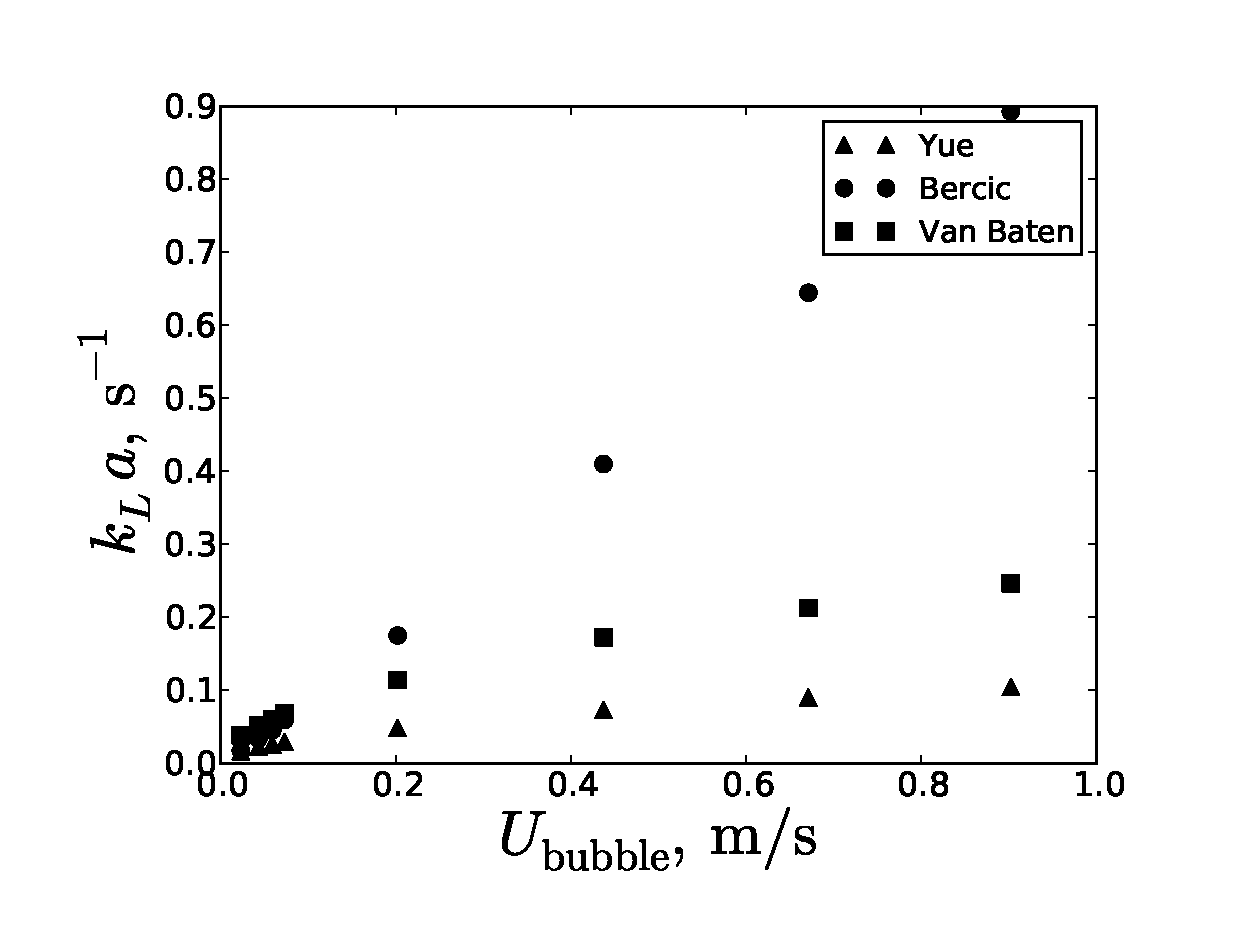
\includegraphics[width=\textwidth]{Figures/theoretical_correlations.eps}\\
%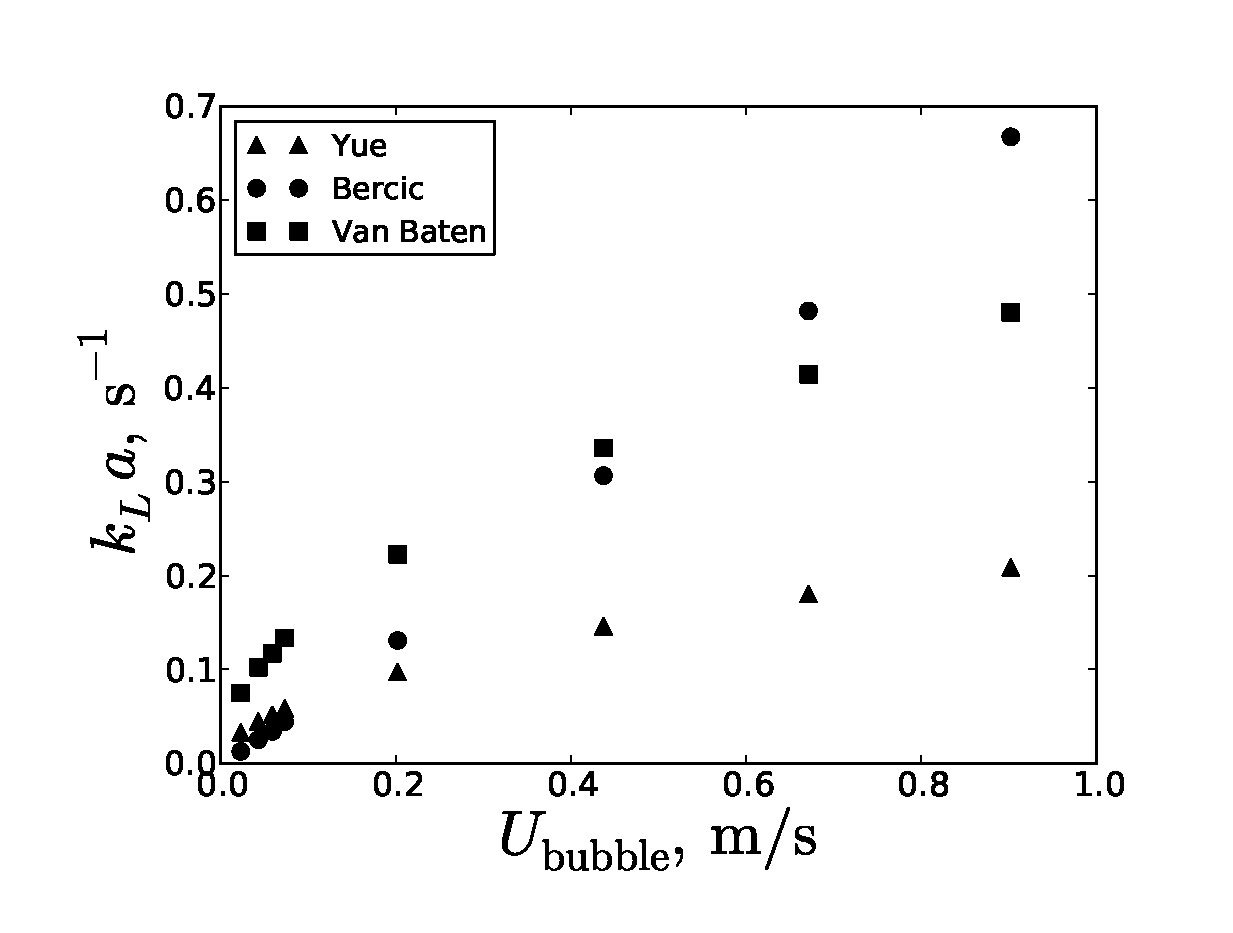
\includegraphics[width=\textwidth]{Figures/theoretical_correlations_without_hydraulic.eps}\\
\caption{The literature correlations by various authors.\label{fig:mass:transfer:theoretical}}
\end{figure}

The volumetric mass transfer coefficient is calculated according to the work of
\citet{vanbaten-circular}. The concentration flux is calculated as the difference between overall
average concentration taken in the whole domain ($C_{overall}=\int_{V} C \mathrm{d}V /V$)
at time
$t_1$ and time $t_2$ divided on the time difference $t_2-t_1$ {\color{red} (In this particular
moment I don't know whether to take the volume of the whole domain or
just the liquid phase. I will go for whole domain.)}. Then the volumetric mass transfer
coefficient is calculated as \cite{vanbaten-circular}:
\begin{equation}
\label{main:simulation:equation}
k_L a=\frac{\text{Flux}}{C_s-C_{outlet}} \frac{\text{bubble surface area}}{\text{unit cell volume}},
\end{equation}
where $C_{outlet}=\int{C U_{outlet}\mathrm{d}A}/\int{U_{outlet}\mathrm{d}A}$. 
{\color{red} Do not understand why we need this ratio bubble surface area/unit cell volume. In this
case the dimensional units do not coincide. In the calculations I will avoid it until further
clearance.} The overall concentration in the lattice Boltzmann system is prescribed as:
\begin{equation}
C_{overall}=\frac{\sum{c_i}}{N_x \, (N_y-2)}.
\end{equation}

To properly do
non-dimensioanalization one needs to insure the time conversion factor when the flux is calculated
inside the lattice Botlzmann system. The time conversion can be easily obtained:
\begin{equation}
\begin{aligned}
&U_{LB}=U_{phys}\frac{\Delta t}{\Delta x}\\
&\Delta t=\frac{U_{LB}}{U_{phys}}\Delta x\\
&\Delta t=\frac{1.5\,\mathrm{mm}}{200} \frac{0.0559}{0.902\,\mathrm{m/s}}=4.64\times
10^{-7}\,\mathrm{s} 
\end{aligned}
\end{equation}

The bubble surface length is the perimeter of the bubble in two-dimensional space and it is
calculated with the extraction of the bubble contour and representing it with the polygon. After
that the calculated perimeter is the effective summation of line lengths and can be represented as:
\begin{equation}
P=\sum_i{\sqrt{(x2_i-x1_i)^2+(y2_i-y1_i)^2}},
\end{equation}
where the index $i$ represents the polyline consisting of two points $(x1,y1)$ and $(x2,y2)$.
%The corresponding volumetric mass transfer coefficients depending on the velocity are indicated in
%Table \ref{table:volumetric:coefficients}.

\section{Comparison between different approaches for one unit cell}
We consequently will examine different approaches to the mass transfer definition, Fig.
\ref{fig:comparison:one:unit:cell}:
\begin{description}
\item[I] Definition of \citet{vanbaten-circular} with periodic boundary conditions where a bubble
is located near the entrance of the computational domain, and the characteristic concentration is
the inlet/outlet concentration, Fig \ref{fig:benchmark}. 
\item[II] Definition of \citet{vanbaten-circular} with periodic boundary conditions where a bubble
is located near the entrance of the computational domain, and the characteristic concentration is
the average concentration, Fig \ref{fig:benchmark}.
\item[III] Definition of \citet{vanbaten-circular} with periodic boundary conditions where a
bubble is located in the middle of the computational domain, and the characteristic concentration
is the inlet/outlet concentration.
\item[IV] Definition of \citet{vanbaten-circular} with periodic boundary conditions where a bubble
is located in the middle of the computational domain, and the characteristic concentration is the
average concentration.
\item[V] Definition with the concentration jump between inlet and outlet over one unit cell.
\end{description}

\begin{figure}[htb!]
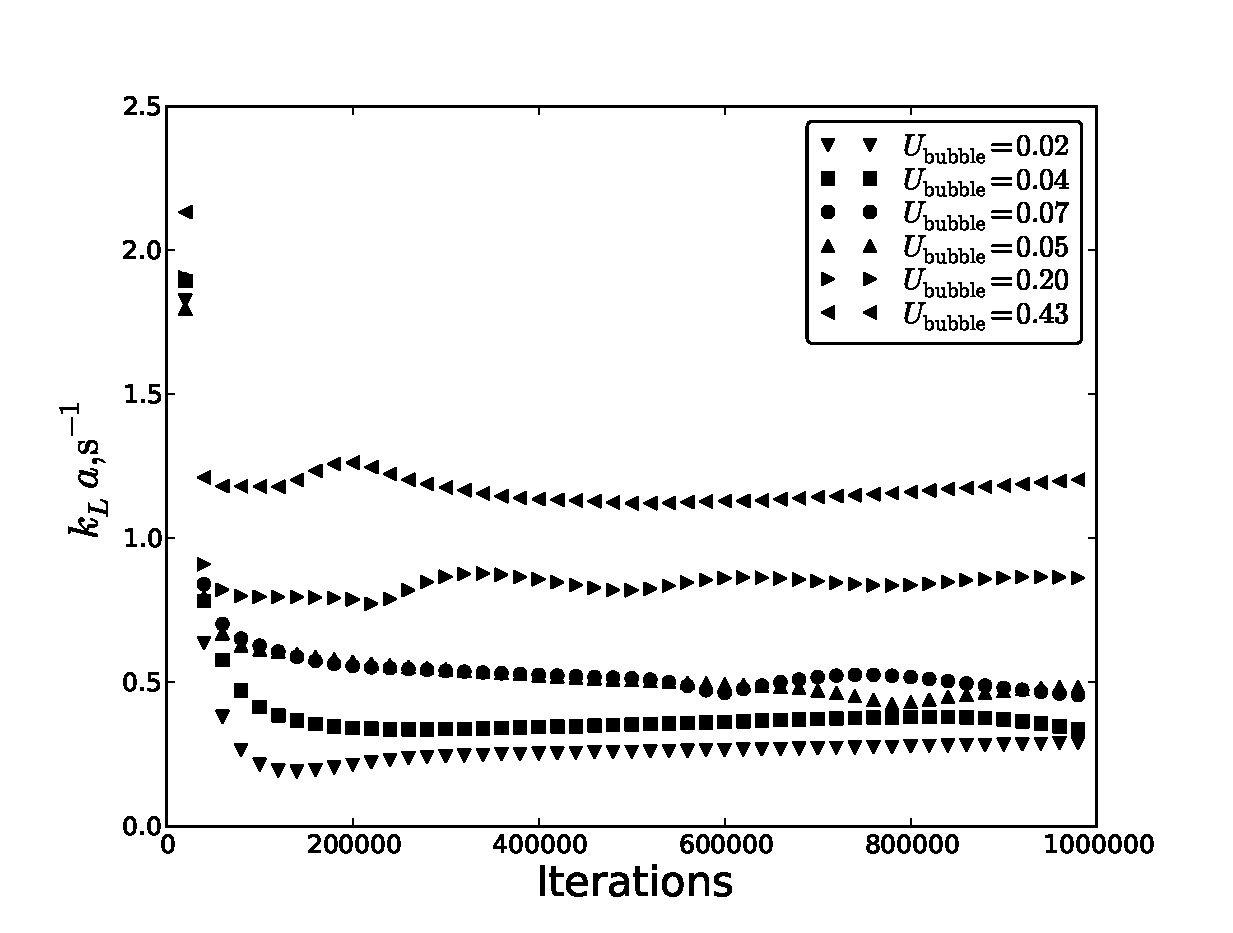
\includegraphics[width=0.5\textwidth]{Figures/steady_state_per_entrance.eps}
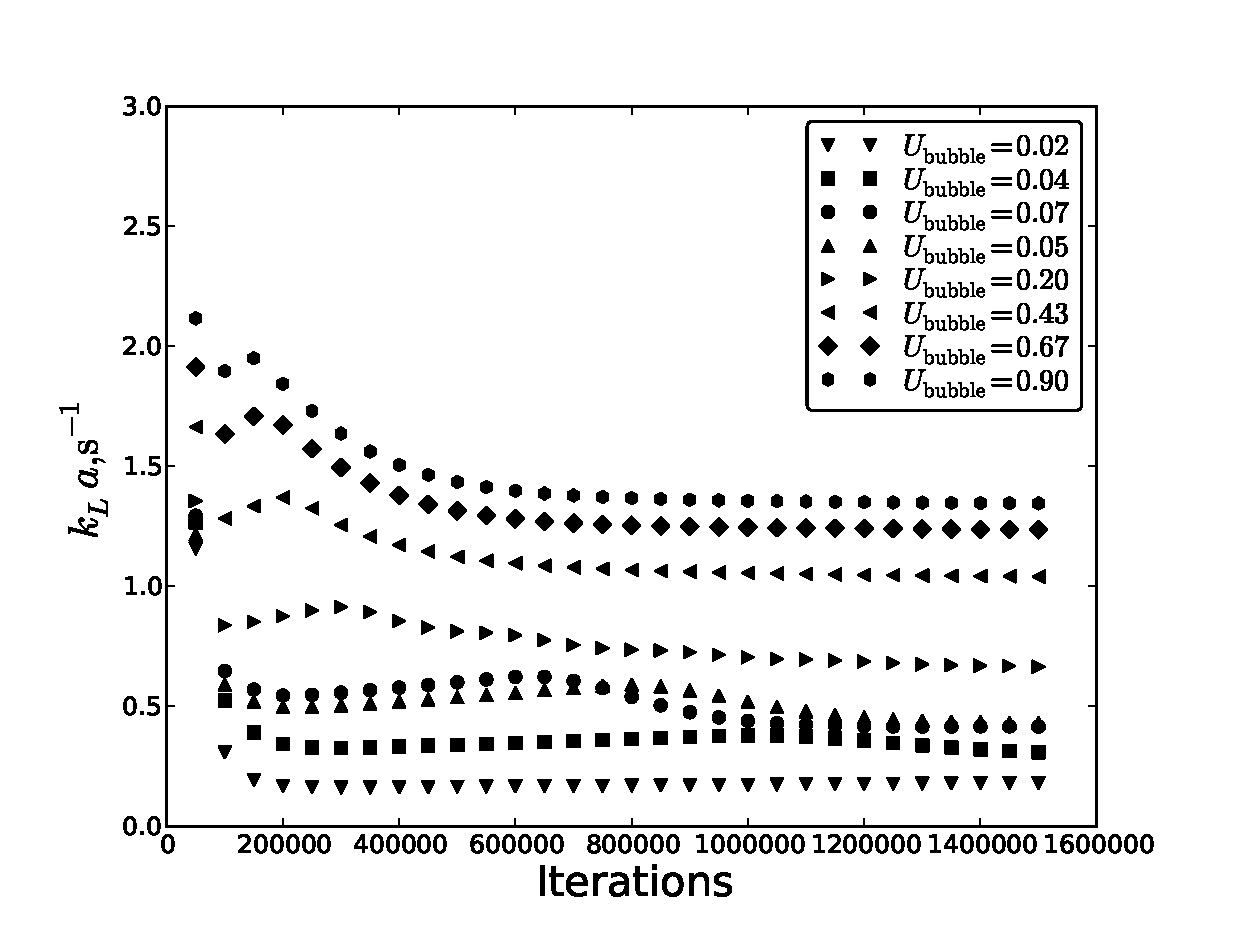
\includegraphics[width=0.5\textwidth]{Figures/steady_state_inlet_aver.eps}\\
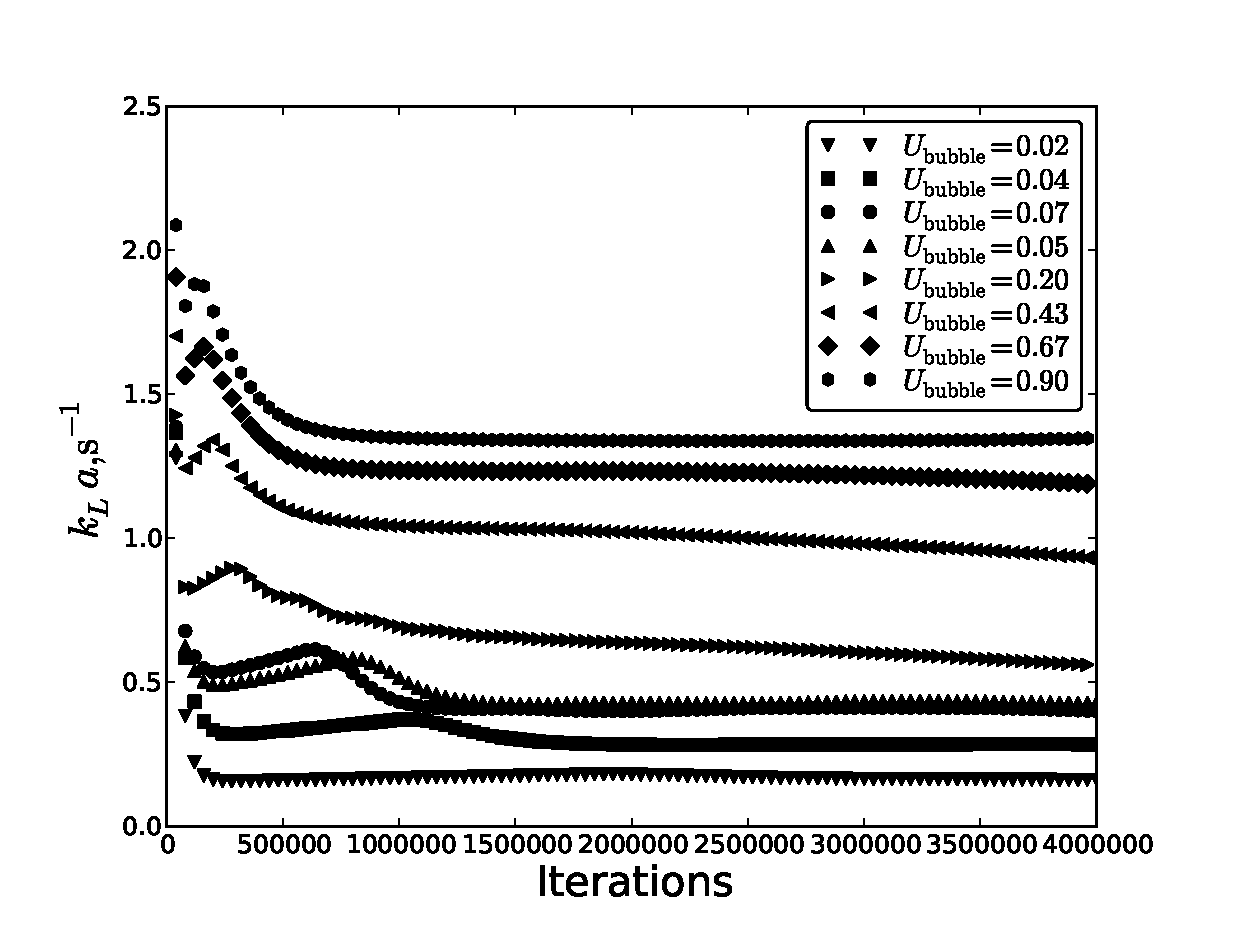
\includegraphics[width=0.5\textwidth]{Figures/steady_state_per_aver.eps}
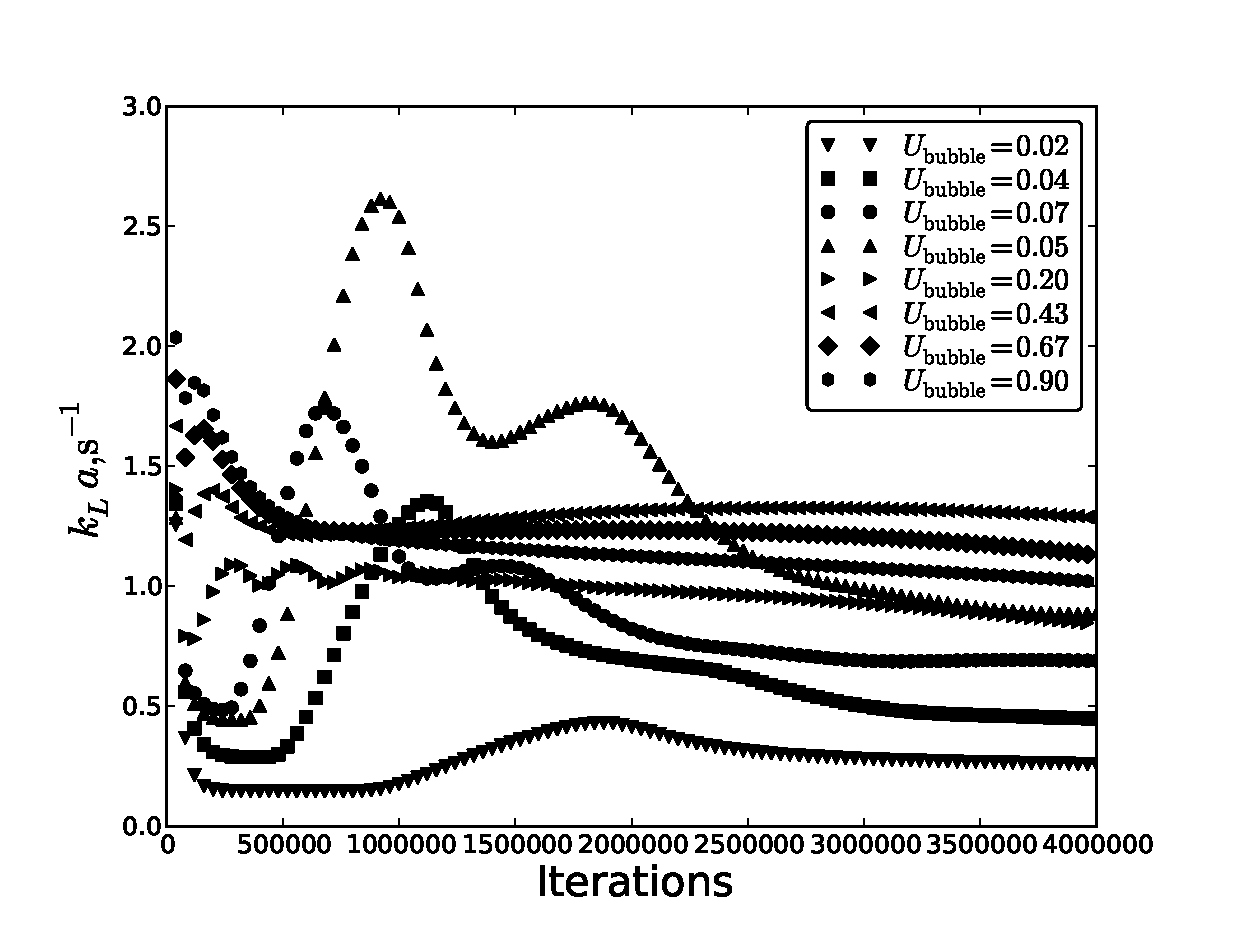
\includegraphics[width=0.5\textwidth]{Figures/steady_state_per_middle_outlet.eps}\\
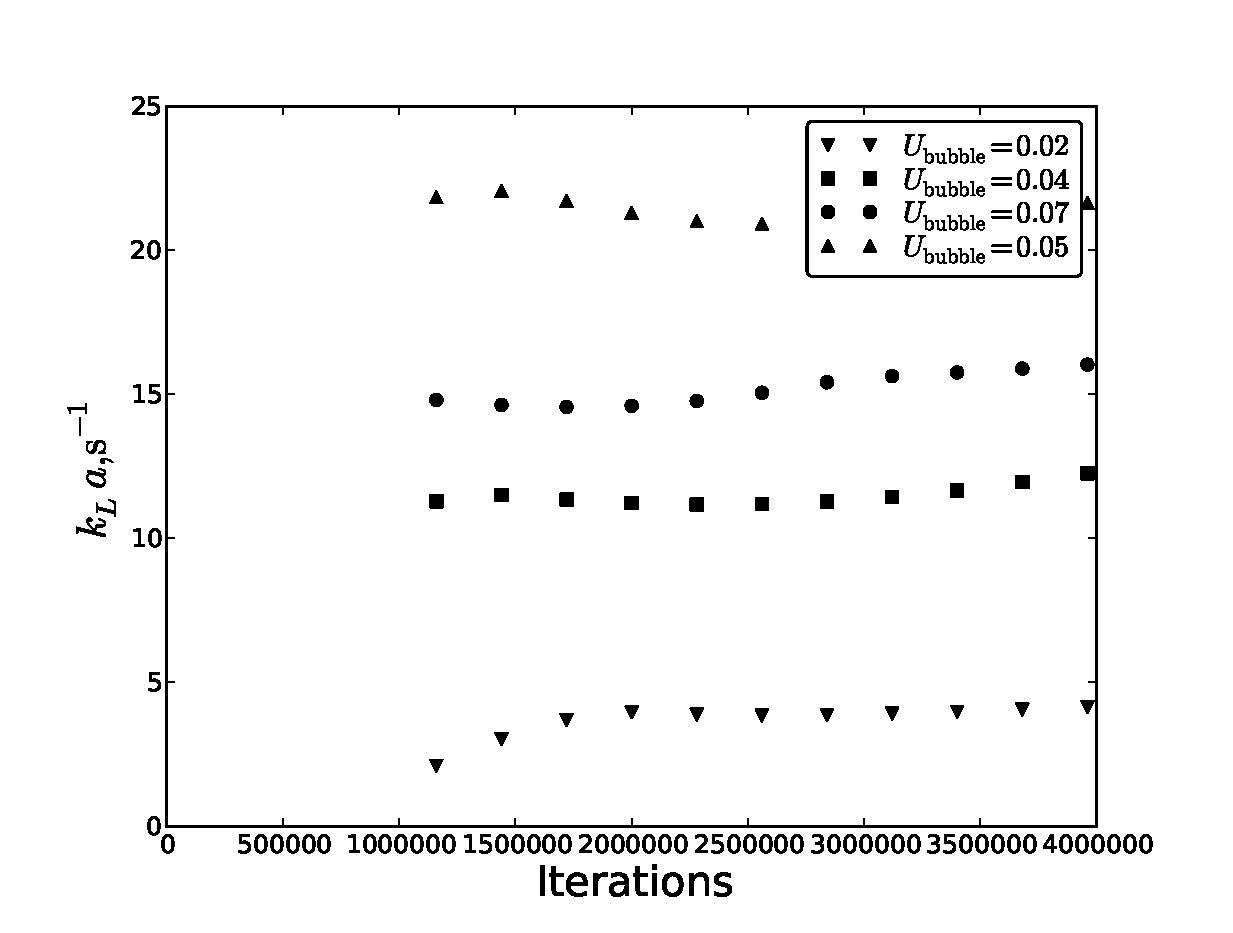
\includegraphics[width=0.5\textwidth]{Figures/steady_state_jos_inlet_outlet.eps}\\
\caption{\label{fig:comparison:one:unit:cell}}
\end{figure}
All the comparison is summarized in Table \ref{table:one_unit_comparison}.
\begin{table}[htb!]
\begin{tabularx}{\textwidth}{|X|X|X|X|X|X|X|X|}
\hline
$Ca$&$Fo$&$\vol_{ent},\,\mathrm{s}^{-1}$&$\vol_{aver},\,\mathrm{s}^{-1}$&$\vol_{mid,
aver},\,\mathrm{s} ^ { -1 }$&$\vol_{mid,out},\,\mathrm{s}^{-1}$&$\vol_{open},\,\mathrm{s}^{-1}$ \\
\hline
$0.026$&$0.08493$&$0.2737$&$0.1775$&$0.1692$&$0.2631$&$3.6756$\\
$0.047$&$0.02160$&$0.3664$&$0.3431$&$0.2852$&$0.4553$&$11.4822$\\
$0.080$&$0.00588$&$0.4959$&$0.4185$&$0.4079$&$0.6920$&$15.1964$\\
$0.065$&$0.00862$&$0.4734$&$0.4517$&$0.4303$&$0.8923$&$21.4517$\\
$0.222$&$0.00103$&$0.8505$&$0.6799$&$0.6109$&$0.8679$&N/A\\
$0.479$&$0.00034$&$1.1541$&$1.0460$&$0.9884$&$1.2995$&N/A\\
$0.736$&$0.00018$&$1.1801$&$1.2395$&$1.2199$&$1.1555$&N/A\\
$0.989$&$0.00012$&$1.2215$&$1.3493$&$1.3400$&$1.0350$&N/A\\
\hline
\end{tabularx}
\caption{Simulation results for different capillary numbers.
\label{table:one_unit_comparison}}
\end{table}
One can see that the only consistent result is for simulations which take into the account average
concentration. The results come to the steady-state after $1,000,000$ iterations. However, to
understand properly what is the real mass transfer coefficient one needs to perform a few units
simultions.

\section{Two unit cells results}
As far as one needs to restore the continuous picture one needs to make a simulation of a few
cells. This section provides results for two units. The results are summarized in Table
\ref{table:two_units}. The results for two sections are presented in Fig. \ref{fig:results:double}.
\begin{figure}[htb!]
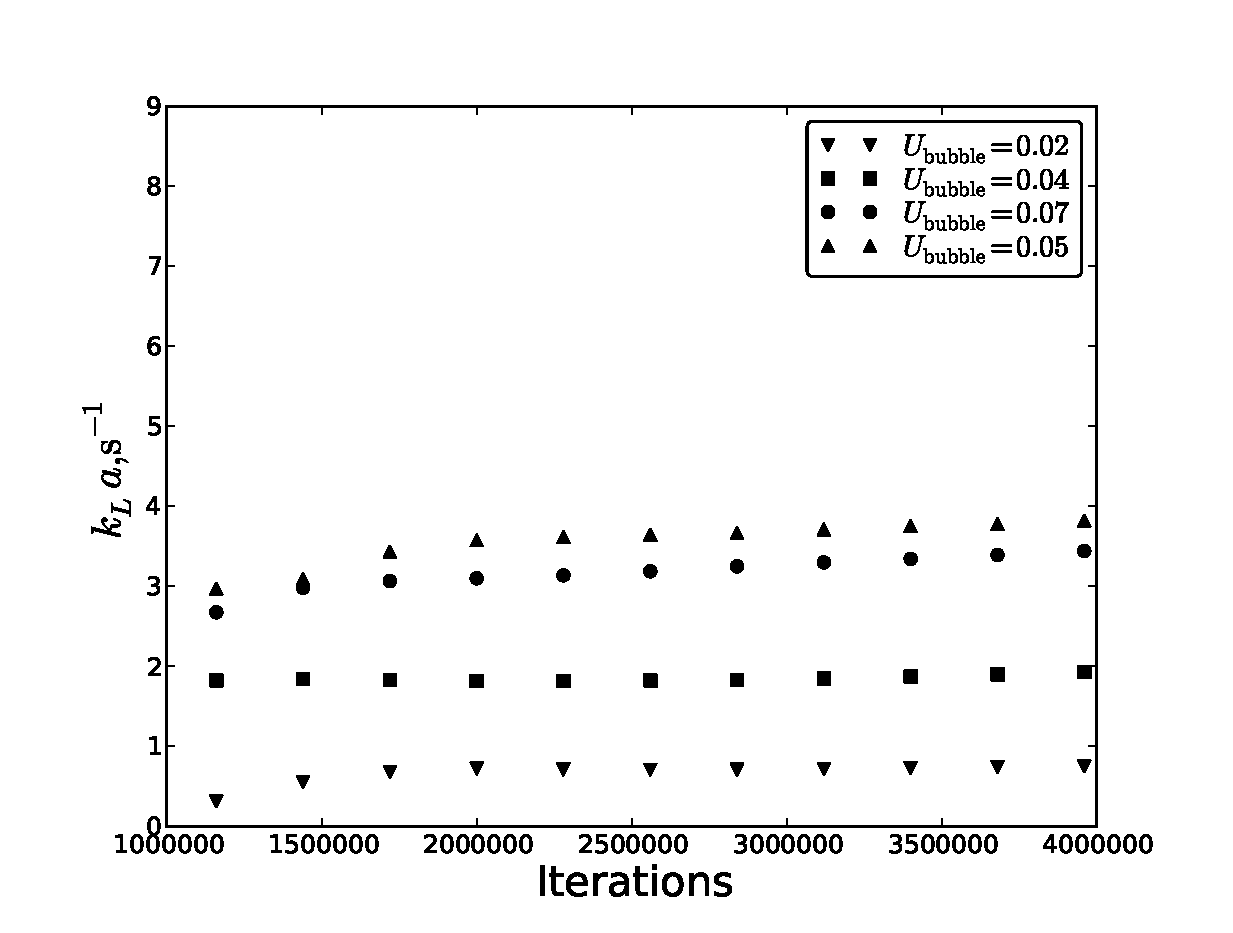
\includegraphics[width=0.5\textwidth]{Figures/steady_double_overall.eps}
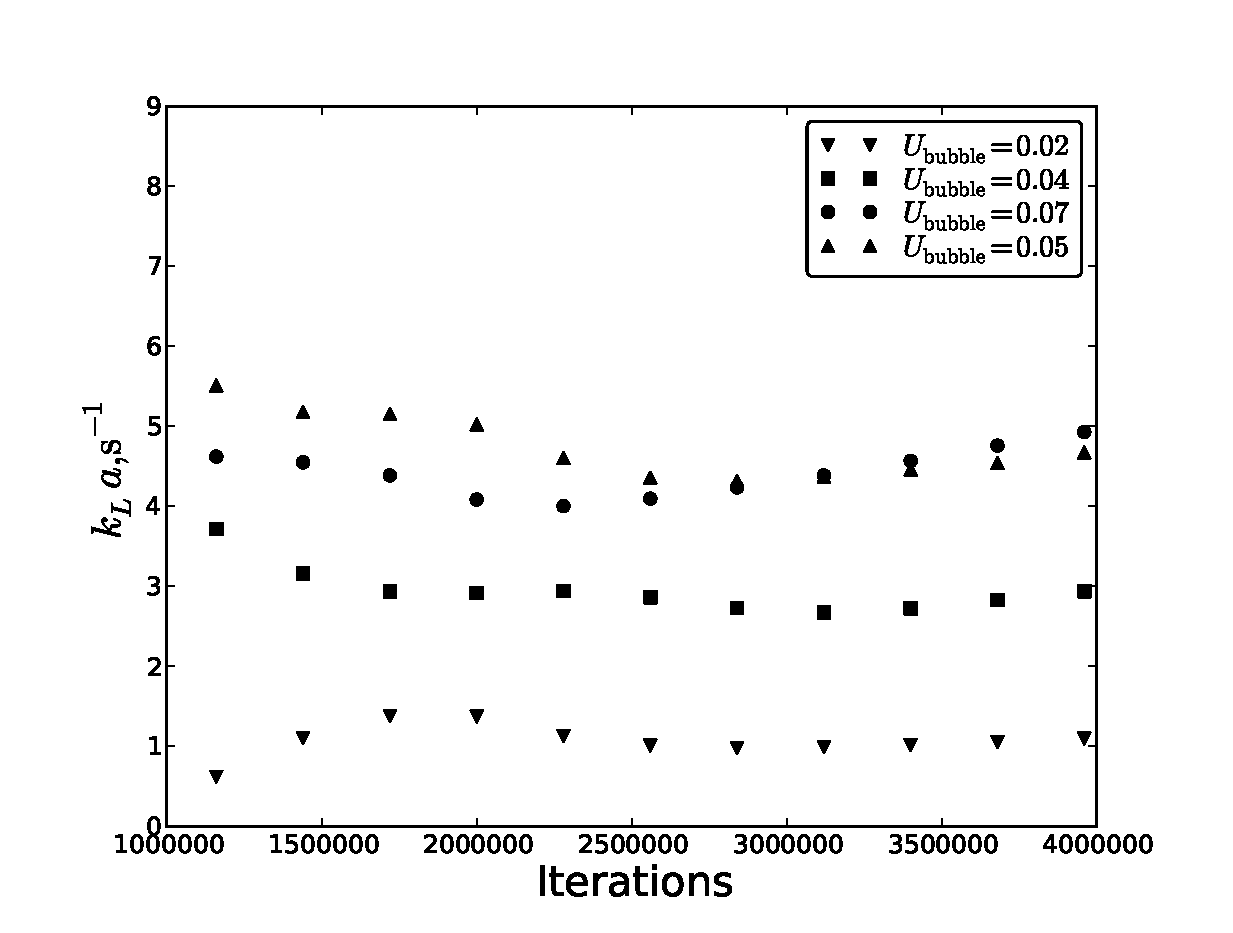
\includegraphics[width=0.5\textwidth]{Figures/steady_double_first.eps}\\
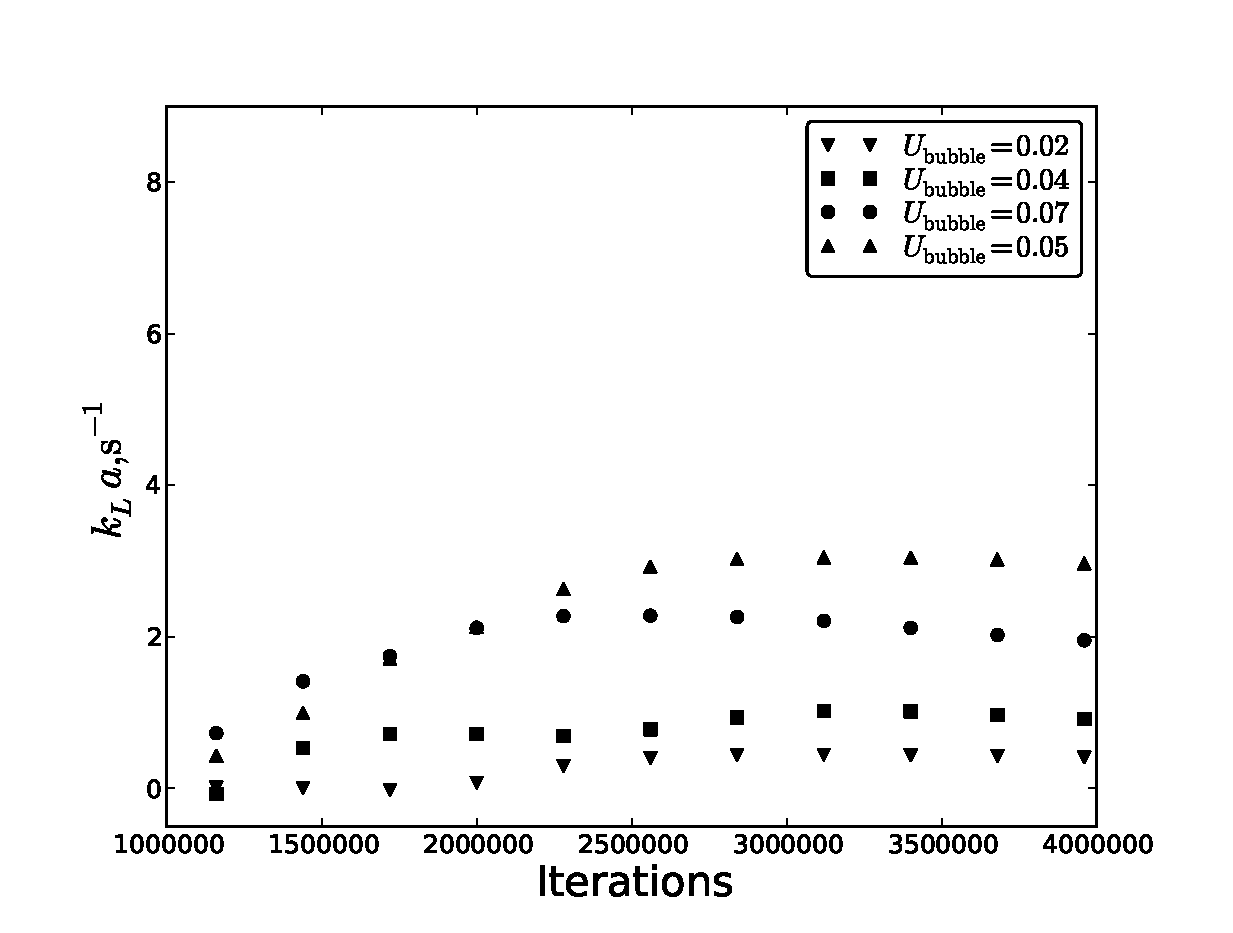
\includegraphics[width=0.5\textwidth]{Figures/steady_double_second.eps}
\caption{Overall mass transfer coefficient (top left), first part (top
right), second part (bottom left).\label{fig:results:double}}
\end{figure}
\begin{table}[htb!]
\begin{tabularx}{\textwidth}{|X|X|X|}
\hline
$0.7392$&$1.0564$&$0.4220$\\
$1.8993$&$2.8301$&$0.9684$\\
$3.3925$&$4.7522$&$2.0328$\\
$3.7870$&$4.5615$&$3.0125$\\
\hline
\end{tabularx}
\caption{Simulation results for two units. \label{table:two_units}}
\end{table}

\section{Three unit cells results}
Three unit cells results are subdivided into three cells. We calculate the mass transfer
coefficients over the each cell, Fig. \ref{fig:results:triple}. The averaged coefficients  after
$3,300,000$ time steps are represented in Table. \ref{table:three_units}. The most important thing
is to look at the third column of the Table \ref{table:three_units} or for at the Fig.
\ref{fig:results:triple} (bottom left). The coefficients for capillary numbers $0.026$ and $0.047$
are almost zero which indicates that the concentration at the first part of the channel is almost
the same as the second part. Thus, there is not enough time steps to transfer concentrate among
whole the channel (plug flow). In comparison with the first two values for capillary number $0.080$
the trend is different and concentrate is spread over the channel. However, the drop coefficients
are still inconsistents. Though last part and the second part exhibit close values (needed to tell
what is the real mass transfer coefficient). Overall, more time steps are needed.
$0.080$
\begin{table}[htb!]
\begin{tabularx}{\textwidth}{|X|X|X|X|}
\hline
0.4928&1.0564&2.8472e-05&0.4219\\
1.2662&2.8301&0.0146&0.9537\\
2.3110&4.7532&1.0665&1.1133\\
\hline
\end{tabularx}
\caption{Simulation results for three units.\label{table:three_units}}
\end{table}
\begin{figure}[htb!]
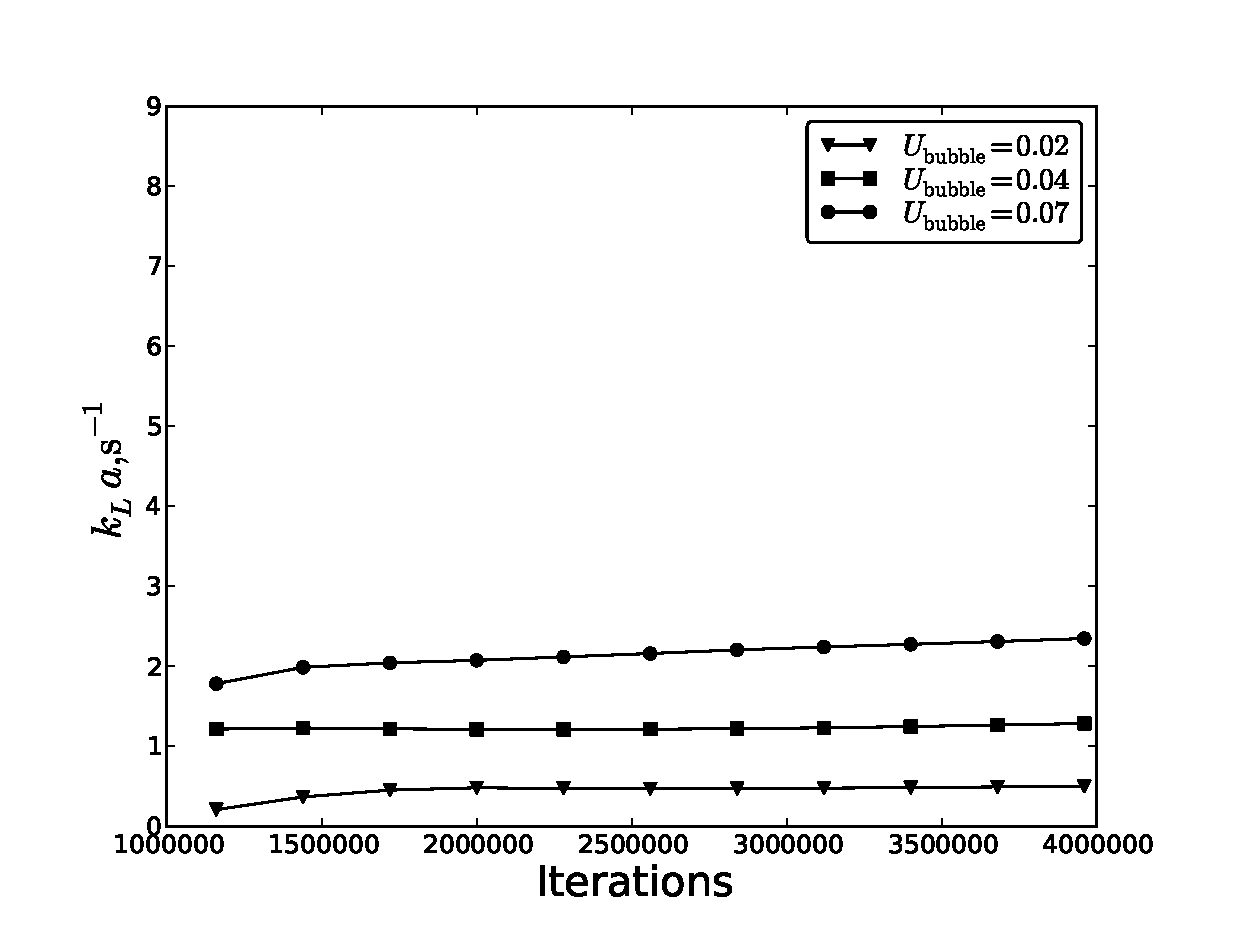
\includegraphics[width=0.5\textwidth]{Figures/steady_triple_overall.eps}
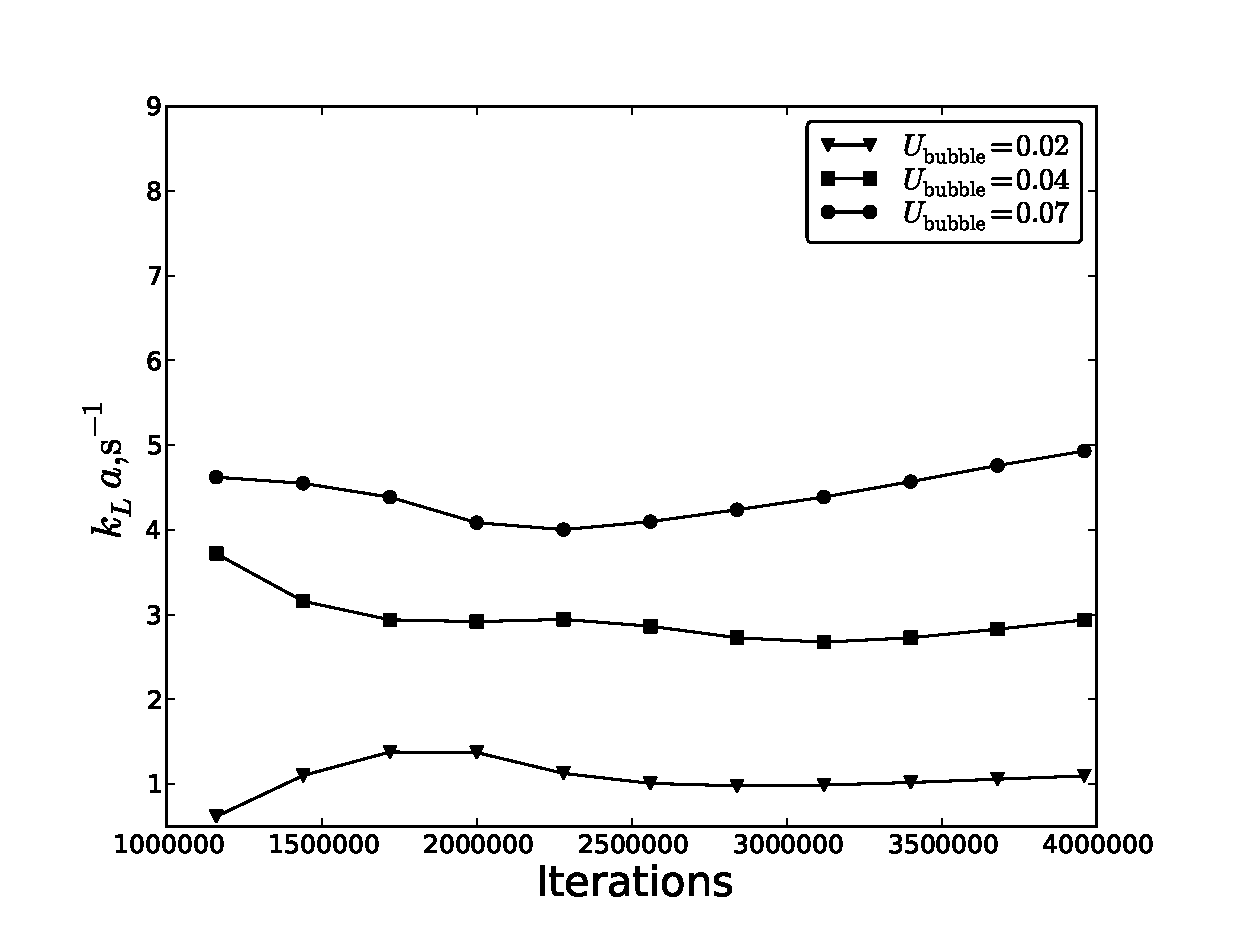
\includegraphics[width=0.5\textwidth]{Figures/steady_triple_first.eps}\\
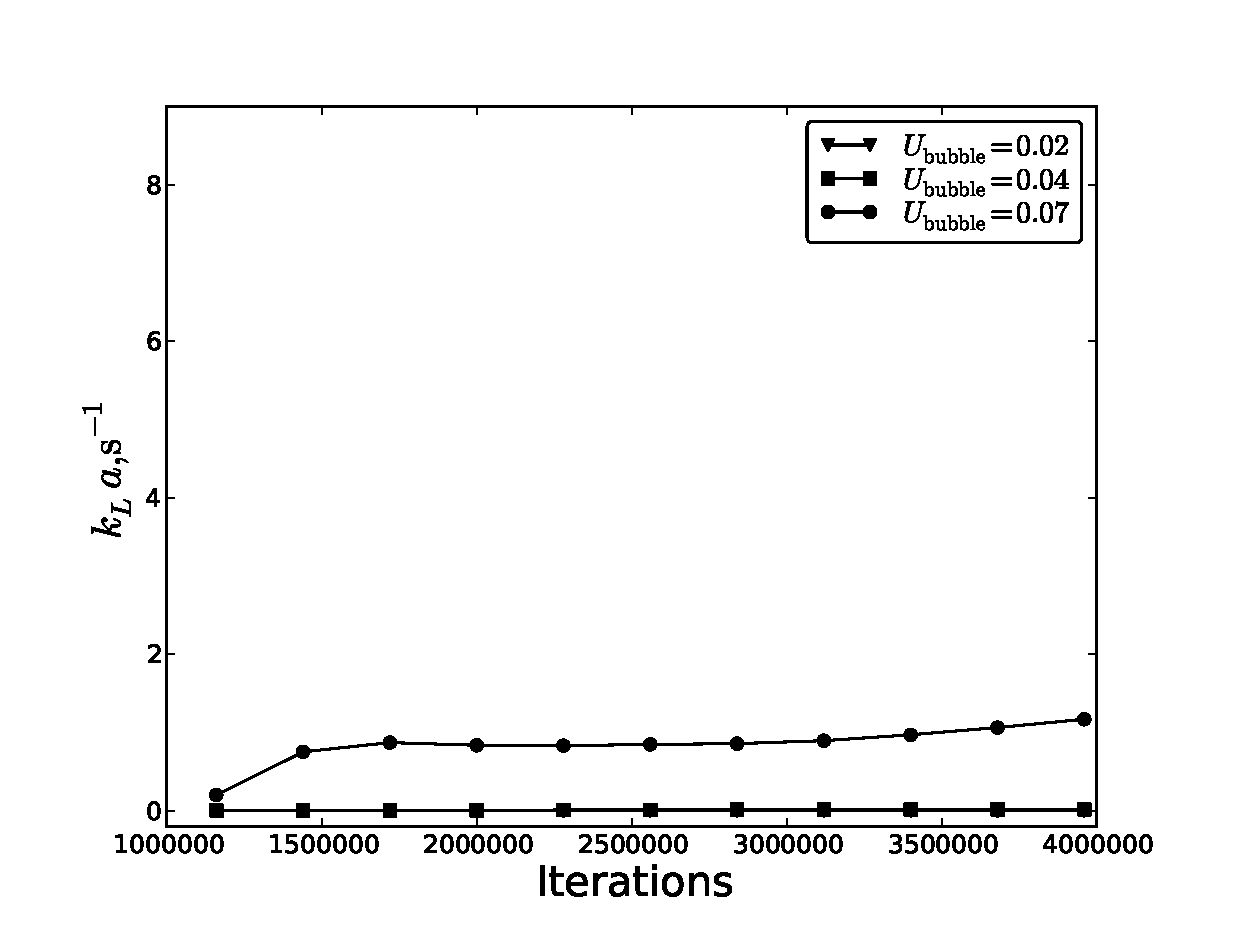
\includegraphics[width=0.5\textwidth]{Figures/steady_triple_second.eps}
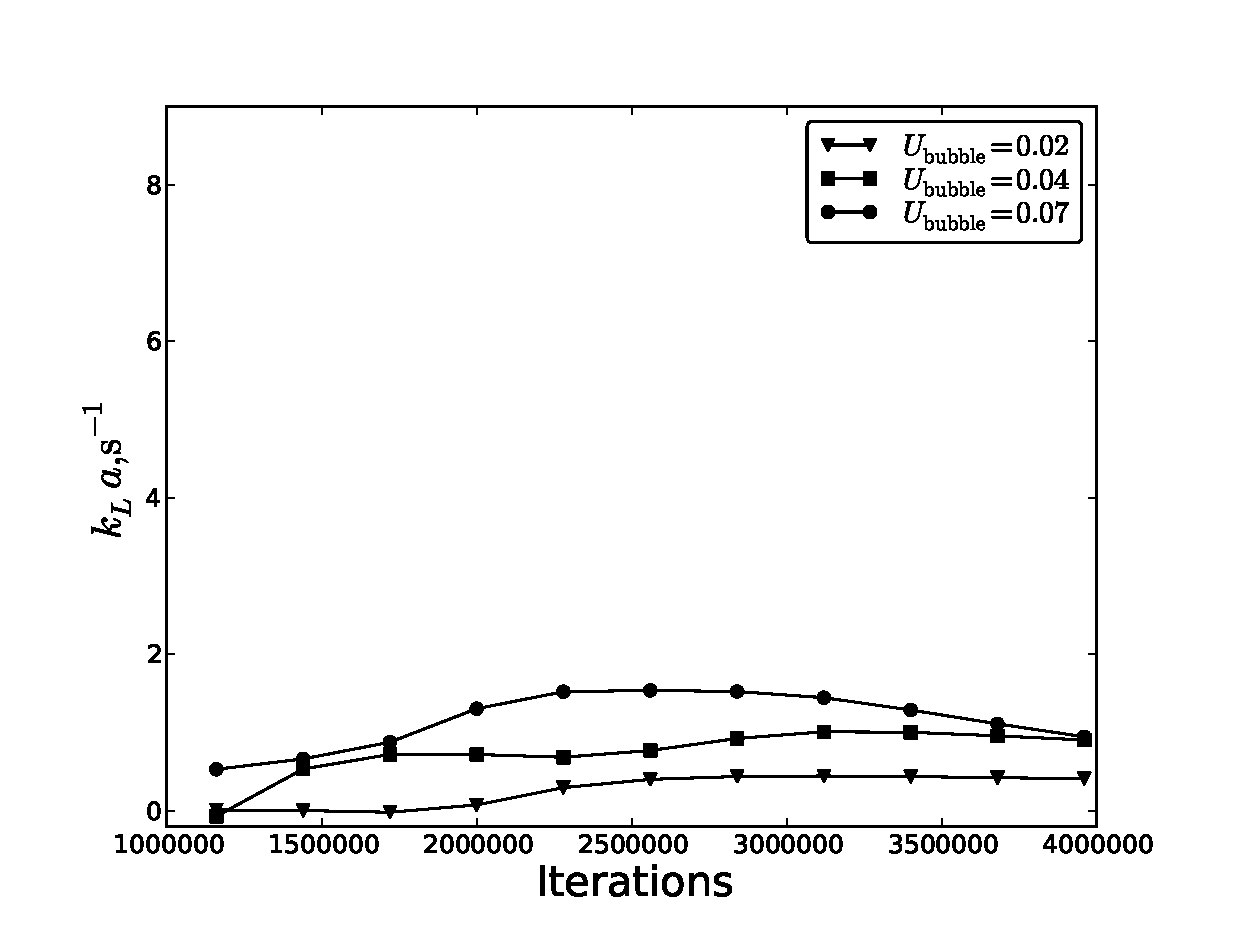
\includegraphics[width=0.5\textwidth]{Figures/steady_triple_third.eps}\\
\caption{The mass transfer coefficient over time in different locations: overall mass transfer
coefficient (top left), first part (top right), second part (bottom left), third part (bottom
right). \label{fig:results:triple}}
\end{figure}

{\color{red} Probably we can consider that for capillary number less than $0.08$ the mass transfer
is a plug flow mass transfer, keeping only the impact from caps.}

\section{Four unit cells results}
Four unit cells results are subdivided into four cells. The results are presented in Fig.
\ref{fig:results:quadro}. While we expect certain deviations for the first and the last part, but
surprisingly the concentration difference over the third segment tends to be zero. That means not
enough time steps are performed. The results over segments are summarized in Table
\ref{table:four_units}.
\begin{table}[htb!]
\begin{tabularx}{\textwidth}{|X|X|X|X|X|X|}
\hline
$Ca$   &Overall  &I       &II      &III     &IV\\
$0.080$&$1.7359$ &$4.7533$&$1.0665$&$0.1088$&$1.0150$\\
$0.065$&$1.9260$ &$4.5620$&$0.9113$&$0.0619$&$2.1689$\\
\hline
\end{tabularx}
\caption{Simulation results for mass transfer coefficients for 4 unit cells
domain.\label{table:four_units}}
\end{table}
\begin{figure}[htb!]
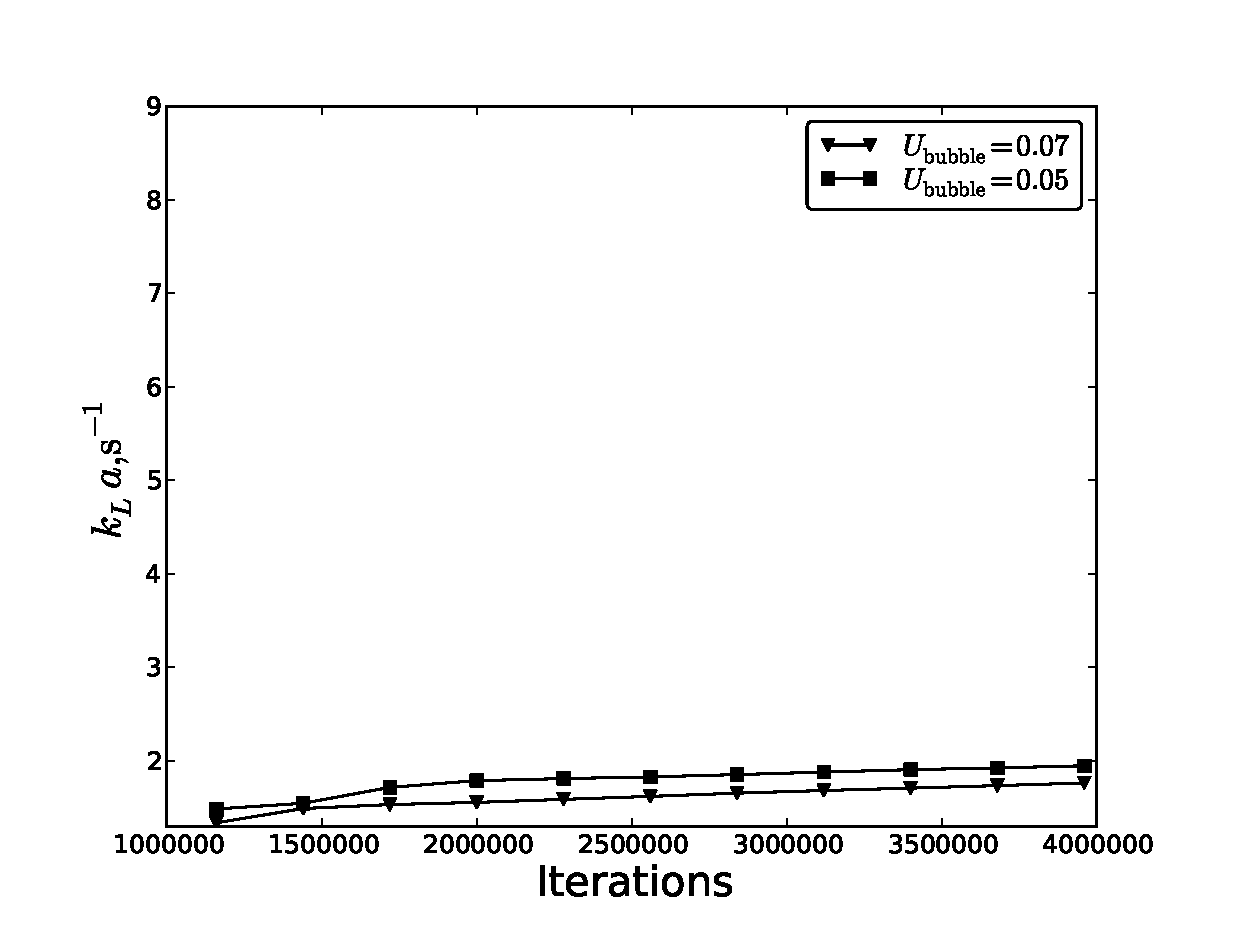
\includegraphics[width=0.5\textwidth]{Figures/steady_quadro_overall.eps}
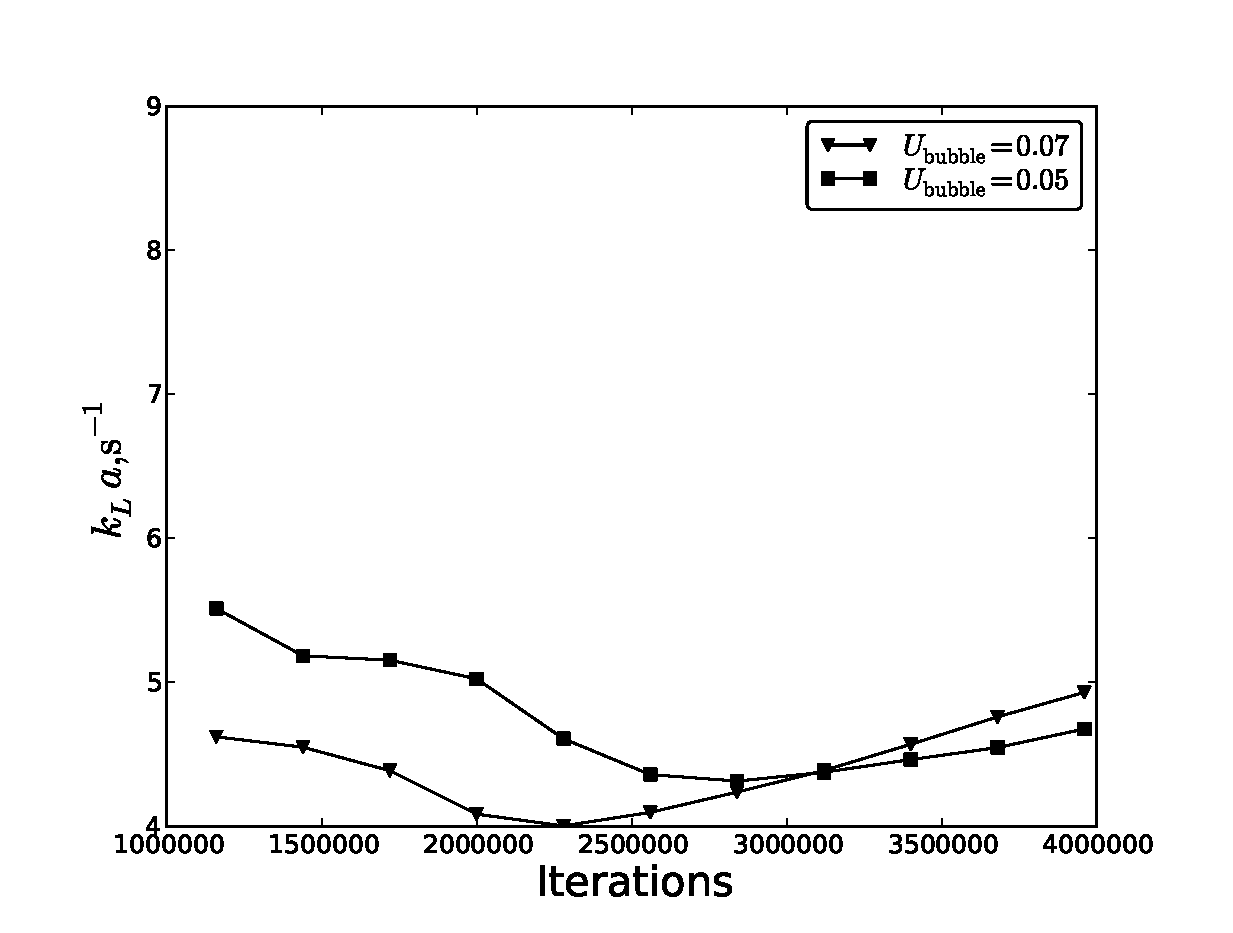
\includegraphics[width=0.5\textwidth]{Figures/steady_quadro_first.eps}\\
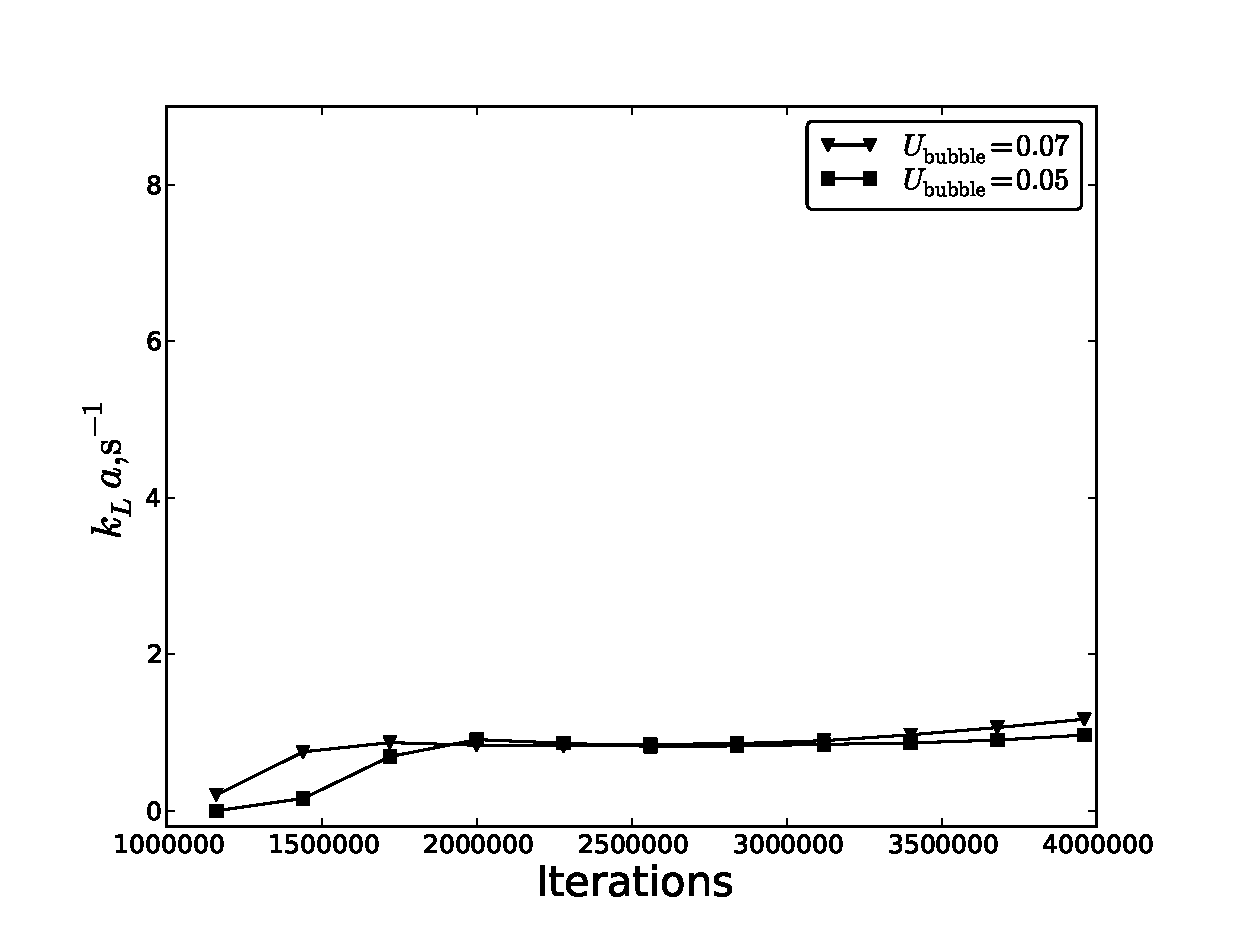
\includegraphics[width=0.5\textwidth]{Figures/steady_quadro_second.eps}
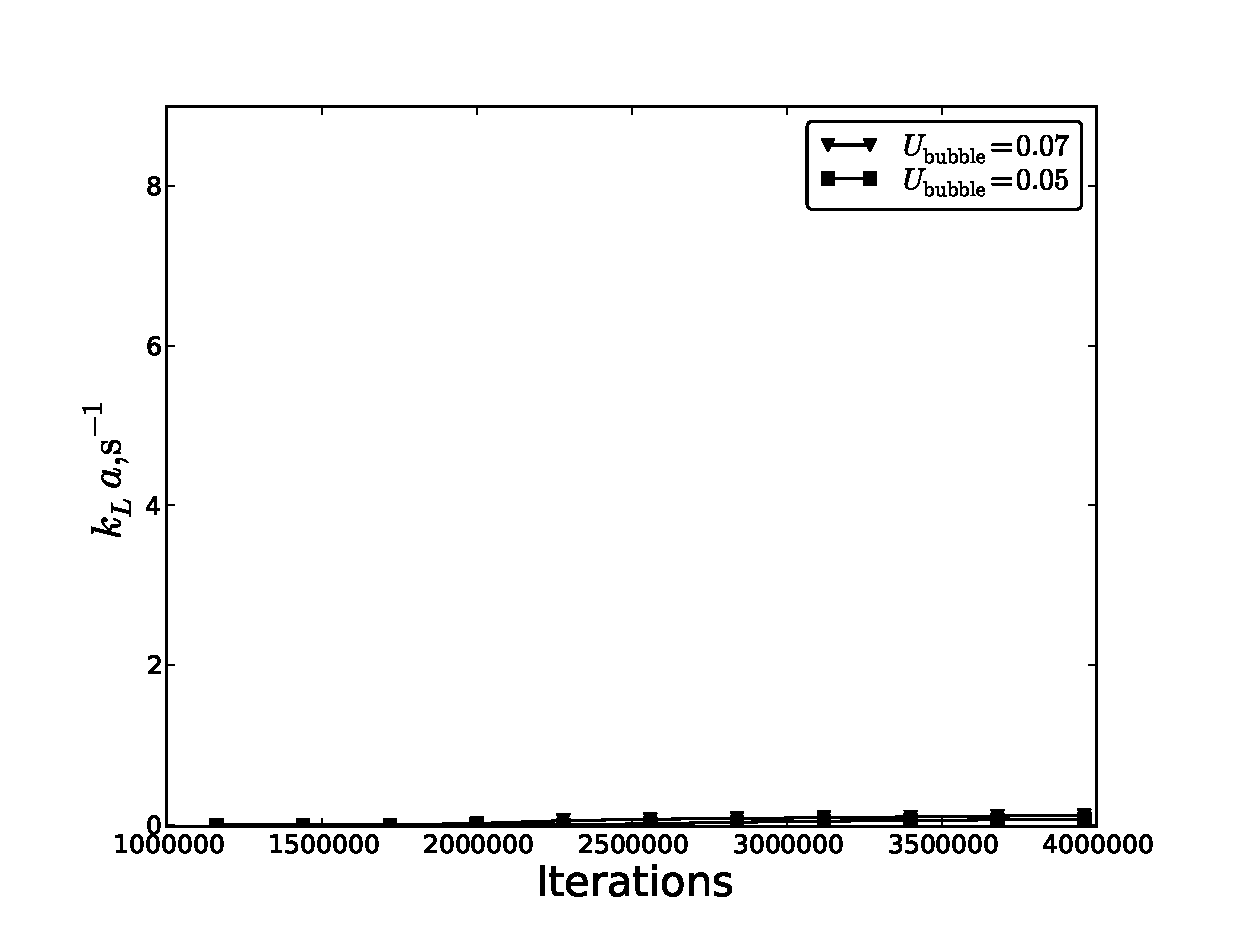
\includegraphics[width=0.5\textwidth]{Figures/steady_quadro_third.eps}\\
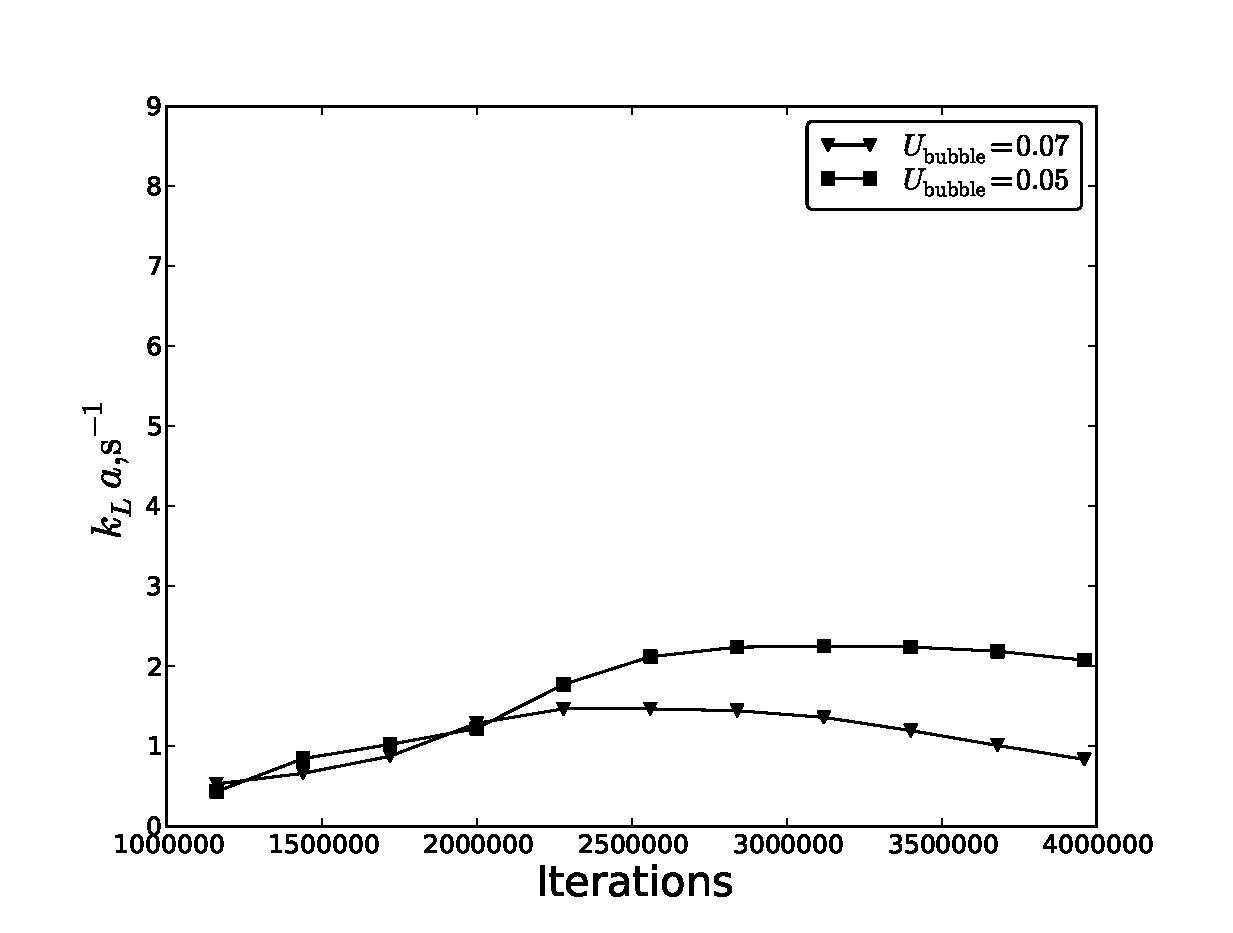
\includegraphics[width=0.5\textwidth]{Figures/steady_quadro_fourth.eps}\\
\caption{The mass transfer coefficient over time in different locations: overall mass transfer
coefficient (top left), first part (top right), second part (middle left), third part (middle
right) and fourth part (bottom left). \label{fig:results:quadro}}
\end{figure}

From Figs. \ref{fig:results:triple} and \ref{fig:results:quadro} one can see that $4,000,000$ time
steps are enough to saturate the second unit for $Ca=0.080$ number. Let us recall bubble velocities
and see what are the characteristic lengths for them calculated as time steps multiplied on the
bubble velocity. From the table one can see that each unit cell is saturated with the timesteps as
$1.5 \frac{N_x}{U_{bubble}}$ {\color{red}(Pretty important result)}. It's inevitably needs the
velocity increase.
\begin{table}[htb!]
\begin{tabularx}{\textwidth}{|X|X|X|X|X|X|X|X|}
\hline
$Ca$ &$U_{bubble}$ &$N_{iter_1}$ &$N_{iter_2}$ &$N_{iter_3}$ &$\frac{L_1}{N_x}$&$\frac{L_2}{N_x}$ 
&$\frac{L_3}{N_x}$\\
$0.026$&$0.0014$&$10^6$&$2\cdot10^6$&$4\cdot10^6$&$0.4666$ &$0.9333$ &$1.8666 $\\
$0.047$&$0.0027$&$10^6$&$2\cdot10^6$&$4\cdot10^6$&$0.9$    &$1.8$    &$3.6    $\\
$0.080$&$0.0045$&$10^6$&$2\cdot10^6$&$4\cdot10^6$&$1.5$    &$3.0$    &$6.0    $\\
$0.065$&$0.0037$&$10^6$&$2\cdot10^6$&$4\cdot10^6$&$1.2333$ &$2.4666$ &$4.9333 $\\
$0.222$&$0.0125$&$10^6$&$2\cdot10^6$&$4\cdot10^6$&$4.1666$ &$8.3333$ &$16.6666$\\
$0.479$&$0.0271$&$10^6$&$2\cdot10^6$&$4\cdot10^6$&$9.0333$ &$18.0666$&$36.1333$\\
$0.736$&$0.0416$&$10^6$&$2\cdot10^6$&$4\cdot10^6$&$13.8666$&$27.7333$&$55.4666$\\
$0.989$&$0.0559$&$10^6$&$2\cdot10^6$&$4\cdot10^6$&$18.6333$&$37.2666$&$74.5333$\\
\hline
\end{tabularx}
\caption{Table results to understand how many time steps are needed to be performed to reach the
saturation.\label{table:time:steps}}
\end{table}

\section{Lattice Boltzmann Benchmarks}

\section{Tweaking velocity}
The reason to tweak velocity is that the velocity field because of the highly nonlinear binary liquid lattice Boltzmann model do not have nice velocity profile, since some streamlines penetrate the bubble in the reference frame of the bubble. Therefore there exists a normal to the surface of the bubble velocity component which destroys right away the advection-diffusion results. Therefore, a special additional free-surface solver was developed in order to dispose the vertical components. 

The solver was through consequent steps. First, we extracted the velocity profiles from the
original binary-liquid simulations. Then, we imposed walls with velocity of the bubble, so the
bubble stays still. At the surface of the bubble the free boundary conditions were imposed, see
\ref{appendix-free-surface}. One of the examples is shown in Fig.
\ref{fig:streamlines:tweaked:velocity}. Among all the simulations the bulk velocity in film and the
slug are different of no more than $7$ percent. {\color{red} Add some pictures froms streamlines.py
if it's required to show more.}
\begin{figure}
\includegraphics[angle=90,width=\textwidth]{Figures/original.eps}\\
\includegraphics[angle=90,width=\textwidth]{Figures/performed.eps}\\
\caption{The comparison between original velocity fields and velocity fields obtained from free surface solver. \label{fig:streamlines:tweaked:velocity}}
\end{figure}


\section{Keeping Peclet}
This section addresses the performance of the simulations. The ulimate goal is to increase
velocity at least by several orders while keeping dimensionless parameters the same. Increasing
velocity can result in simulations of a lot of unit cells required for continuous picture
representation.

Only nondimensional parameter Peclet number governs the advection-diffusion equation:
\beq
Pe=\frac{U_{bubble} N_y}{D},
\feq
where $D$ is the diffusion coefficient to prescribe. As far as we want to increase velocity, that
means one needs to increase the diffusion coefficient as well. The runs were made with
velocities $2,4,6,8,10,15,20,40$ times larger than original velocities. The velocities we chose and
its corresponding capillary numbers are presented in Table \ref{table:scaling:peclet}. Periodic
boundary conditions were used and mass transfer coefficient was calculated according to Eq.
(\ref{main:simulation:equation}).
\begin{table}[htb!]
\begin{tabularx}{\textwidth}{|X|X|X|X|}
\hline
Scale&$U_{bubble}$&Time Iterations&$C_{aver}$\\
\hline
\multicolumn{4}{c}{}\\
\multicolumn{4}{c}{$Ca=0.097$}\\
\hline
$2$ &$0.011$&$400000$&$0.318$\\
$4$ &$0.023$&$200000$&$0.319$\\
$8$ &$0.044$&$100000$&$0.320$\\
$10$&$0.055$&$80000$ &$0.321$\\
$20$&$0.11 $&$40000$ &$0.324$\\
$40$&$0.22 $&$20000$ &$0.328$\\
\hline
\multicolumn{4}{c}{}\\
\multicolumn{4}{c}{$Ca=0.254$}\\
\hline
$2$& $0.0286$&$800000$&$0.6533$\\
$4$& $0.0572$&$400000$&$0.6591$\\
$8$& $0.1144$&$200000$&$0.6692$\\
$10$&$0.1430$&$160000$&$0.6734$\\
$20$&$0.2860$&$80000$ &$0.6894$\\
\hline
\multicolumn{4}{c}{}\\
\multicolumn{4}{c}{$Ca=0.526$}\\
\hline
$2$&$0.0594$&$200000$&$0.3271$\\
$4$&$0.1188$&$100000$&$0.3315$\\
\hline
\multicolumn{4}{c}{}\\
\multicolumn{4}{c}{$Ca=0.750$}\\
\hline
$2$&$0.0848$&$200000$&$0.3489$\\
\hline
\multicolumn{4}{c}{}\\
\multicolumn{4}{c}{$Ca=1.040$}\\
\hline
$2$&$0.1176$&$200000$&$0.3675$\\
\hline
\end{tabularx}
\caption{Scaling Peclet table. One can see that scaling is pretty successful. One can see as well
that the stability limit is approximately around $U_{bubble}=0.1$. That can give us an idea of
scale of simulations. \label{table:scaling:peclet}}
\end{table}

The corresponding to Table \ref{table:scaling:peclet} contour profiles for different scalings are
presented in Fig. \ref{fig:contours:scaling:peclet}.
\begin{figure}
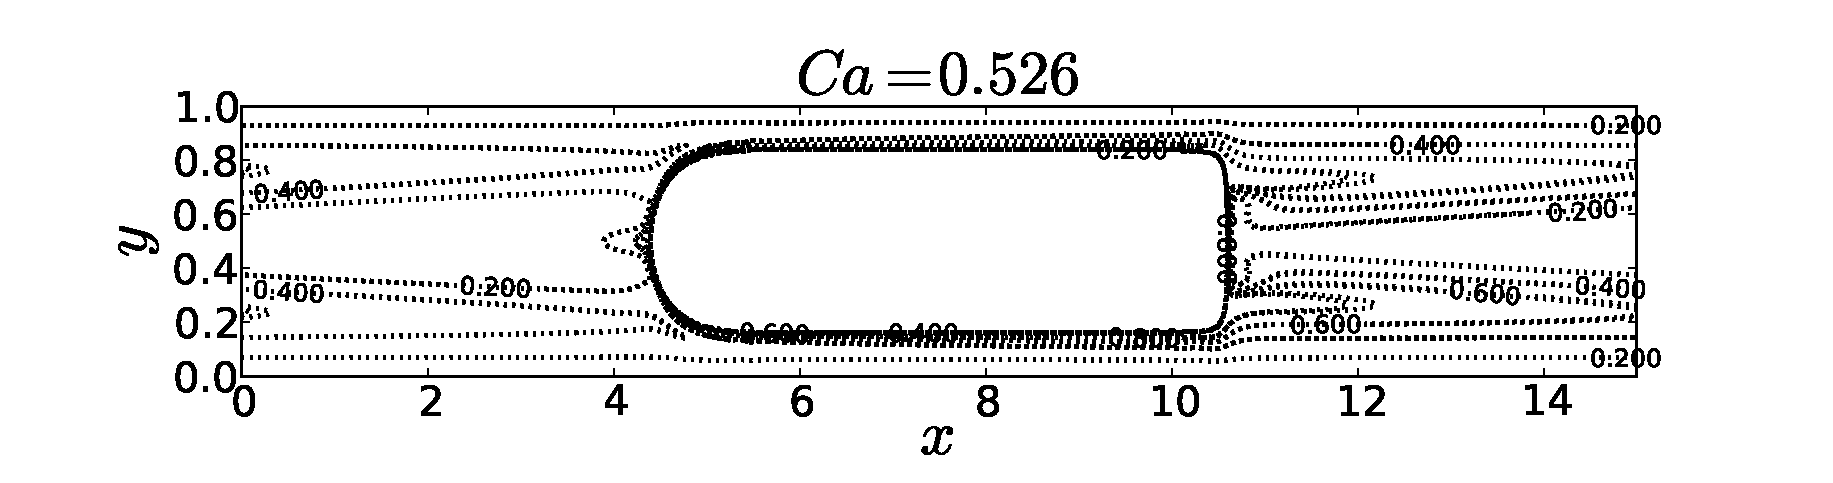
\includegraphics[height=0.3\textwidth]{Figures/contourlines_scale_ca026.eps}\\
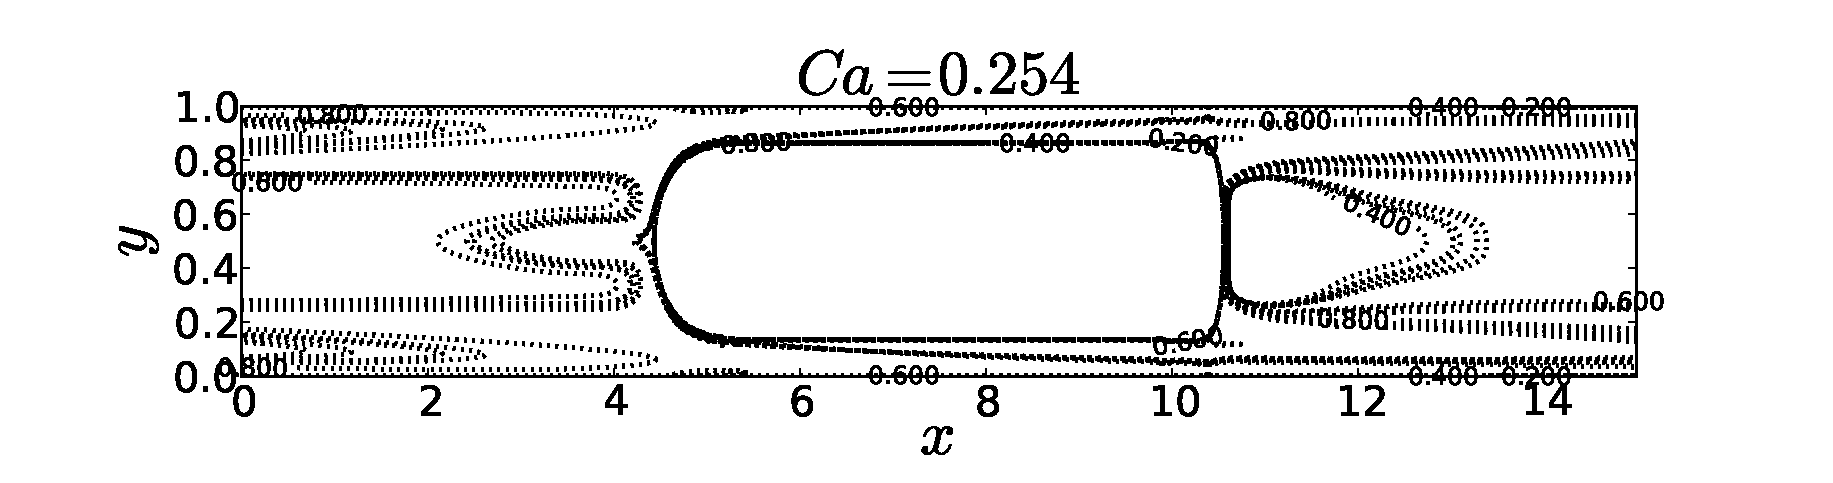
\includegraphics[height=0.3\textwidth]{Figures/contourlines_scale_ca054.eps}\\
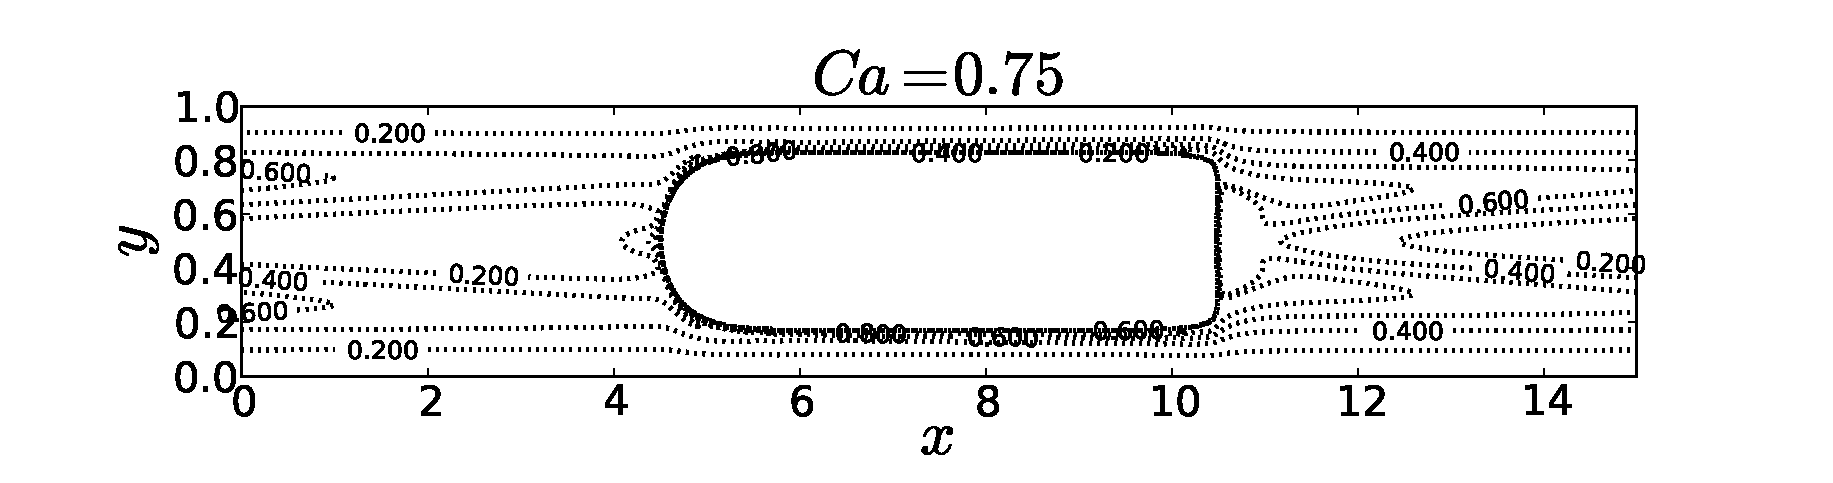
\includegraphics[height=0.3\textwidth]{Figures/contourlines_scale_ca05.eps}\\
\includegraphics[height=0.3\textwidth]{Figures/contourlines_scale_ca097.eps}\\
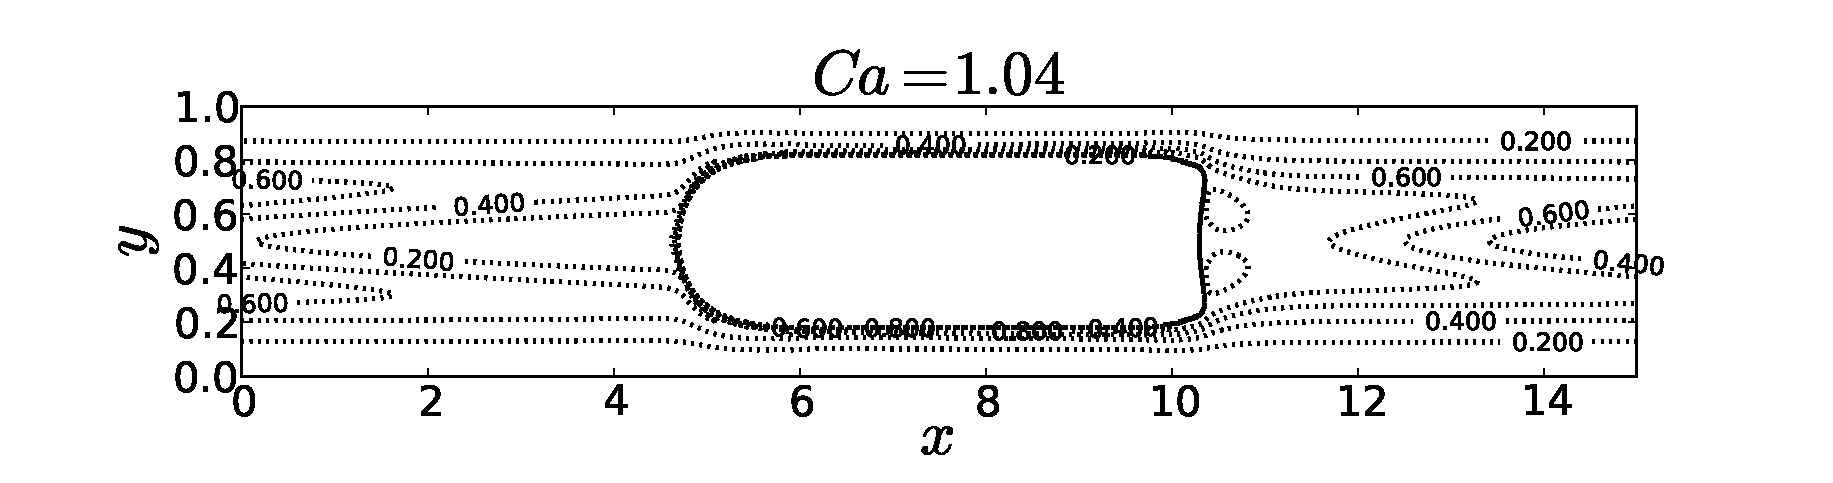
\includegraphics[height=0.3\textwidth]{Figures/contourlines_scale_ca14.eps}\\
\caption{Contours for scaling Peclet number.\label{fig:contours:scaling:peclet}}
\end{figure}

\section{Performing real simulations}
As it was found earlier one needs to make a few units simulations to obtain a proper volumetric
mass transfer coefficient. This section studies the quantity of the unit cells on the volumetric
mass transfer coefficient to be independent of the number of unit cells. The cases we want to
examine in terms of the capillary number are indicated above. The number of cells we want to
simulate are $1$,$4$,$6$,$8$,$10$. As it was discussed in the previous section we want to keep
velocity around $0.05-0.1$. The number of steps for mass to cross whole domain is approximately
$1.5 \frac{N_x}{U_{bubble}}$, given the bulk velocity. If $U_{bubble}$ is taken as $0.05$ then for
the domain size $3000$ one can obtain the following number of iteration for mass transfer to be
stabilize $1.5 \frac{3000}{0.05}=90000$. Therefore, $10^{6}$ time iterations are enough for system
to be stabilized.



%For $Ca=0.0055$ a few results are given in Fig. \ref{fig:ca0055:keeping:peclet}. The rule of the
%thumb that for such simulations the velocity shouldn't be more than $0.05$.

%\begin{figure}[htb!]
%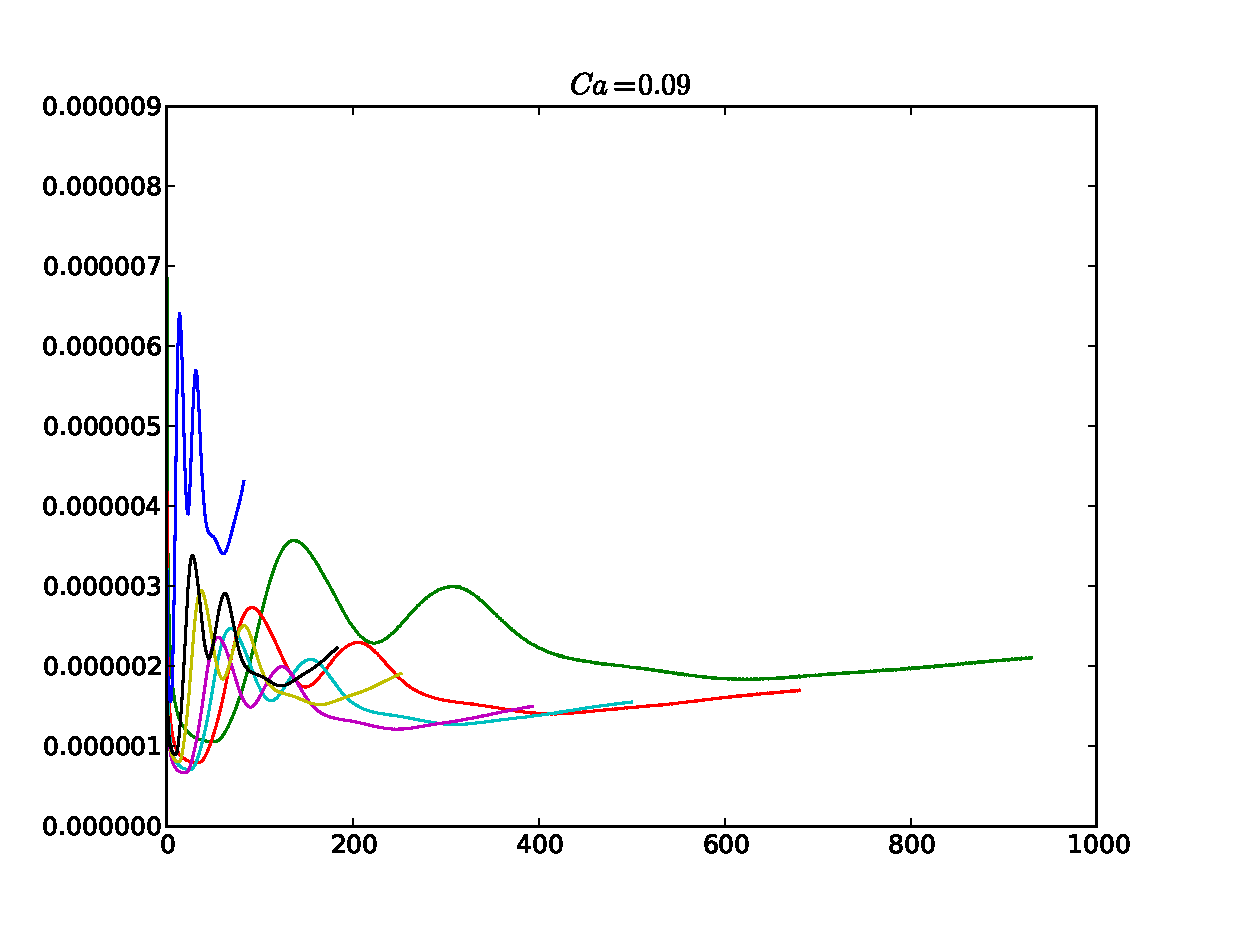
\includegraphics[width=\textwidth]{Figures/scalingpeclet009.eps}
%\caption{The same Peclet number for $Ca=0.0055$. One can see that
%the mass transfer coefficient comes to the same point.{\color{red} Need to compare contours for the
%concentration!!!} \label{fig:ca0055:keeping:peclet}}
%\end{figure}

\section{Performing average approach}
One can calculate the average domain concentration over the time. According to the definitions of
the volumetric mass transfer coefficient one can obtain the following concentration depending on
time, i.e. streamwise coordinate:
\beqal
&\vol t \frac{\ububble}{\ugas+\uliq}=\ln\frac{C^*}{C^*-C(t)}\\
&\vol \frac{\lunit}{\ugas+\uliq}=\frac{\lunit}{\ububble t} \ln \frac{C^*}{C^*-C(t)}\\
\feqal
Simulations for coefficient $\vol \frac{\ububble}{\ugas+\uliq}$ are shown in Fig.
\ref{fig:aver:conc:different:capillaries}.
\begin{figure}
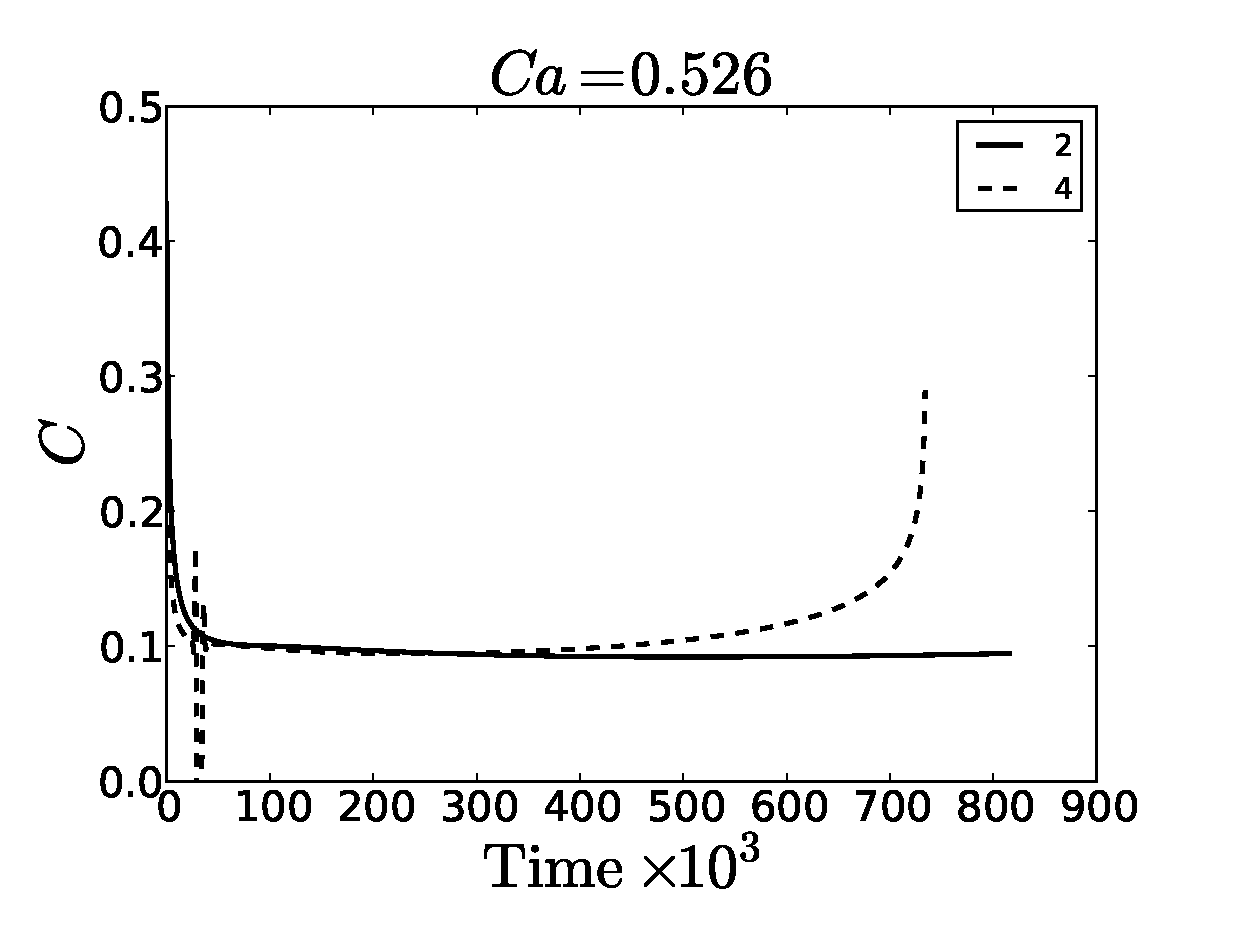
\includegraphics[width=0.5\textwidth]{Figures/aver_conc_scale_ca026.eps}
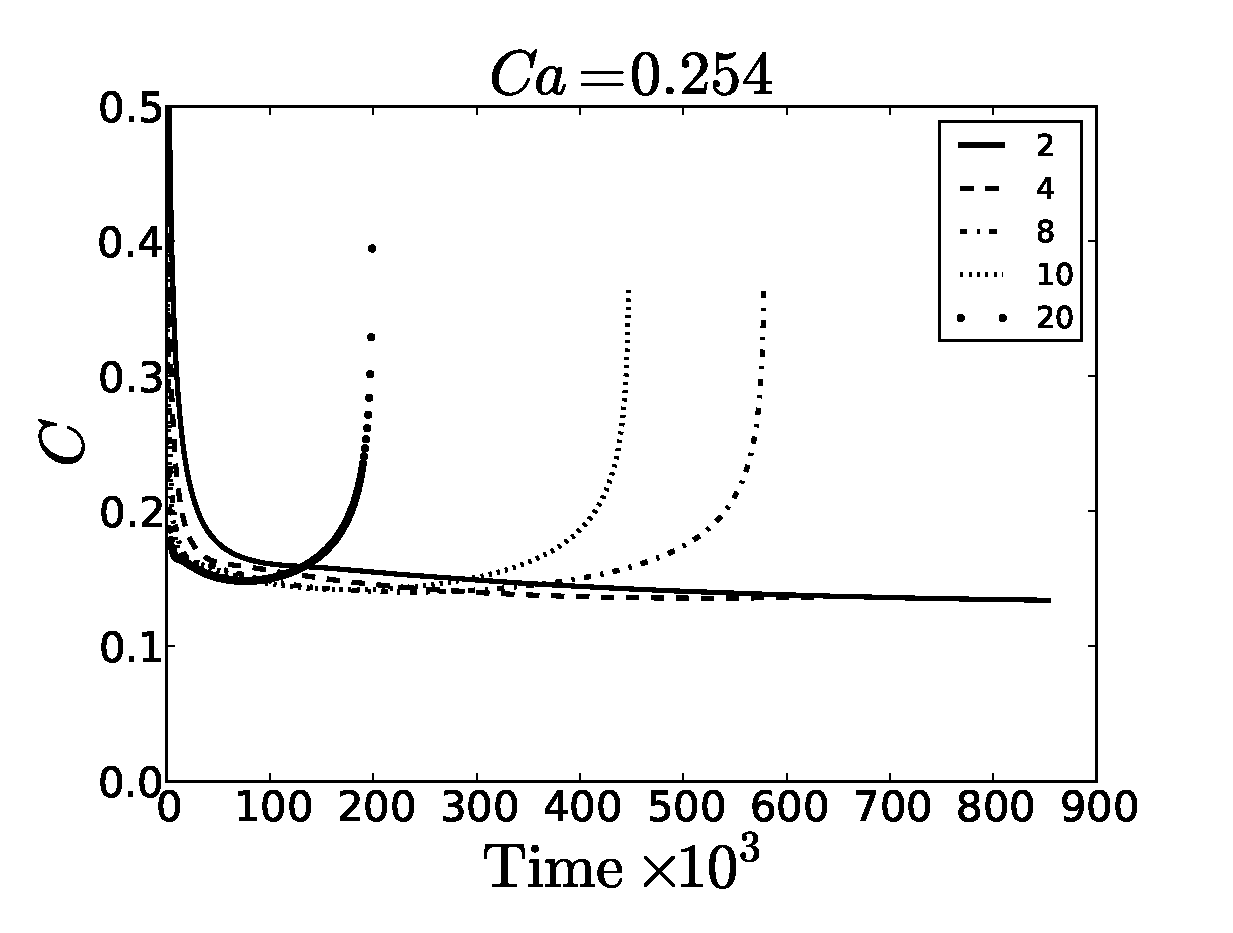
\includegraphics[width=0.5\textwidth]{Figures/aver_conc_scale_ca054.eps}\\
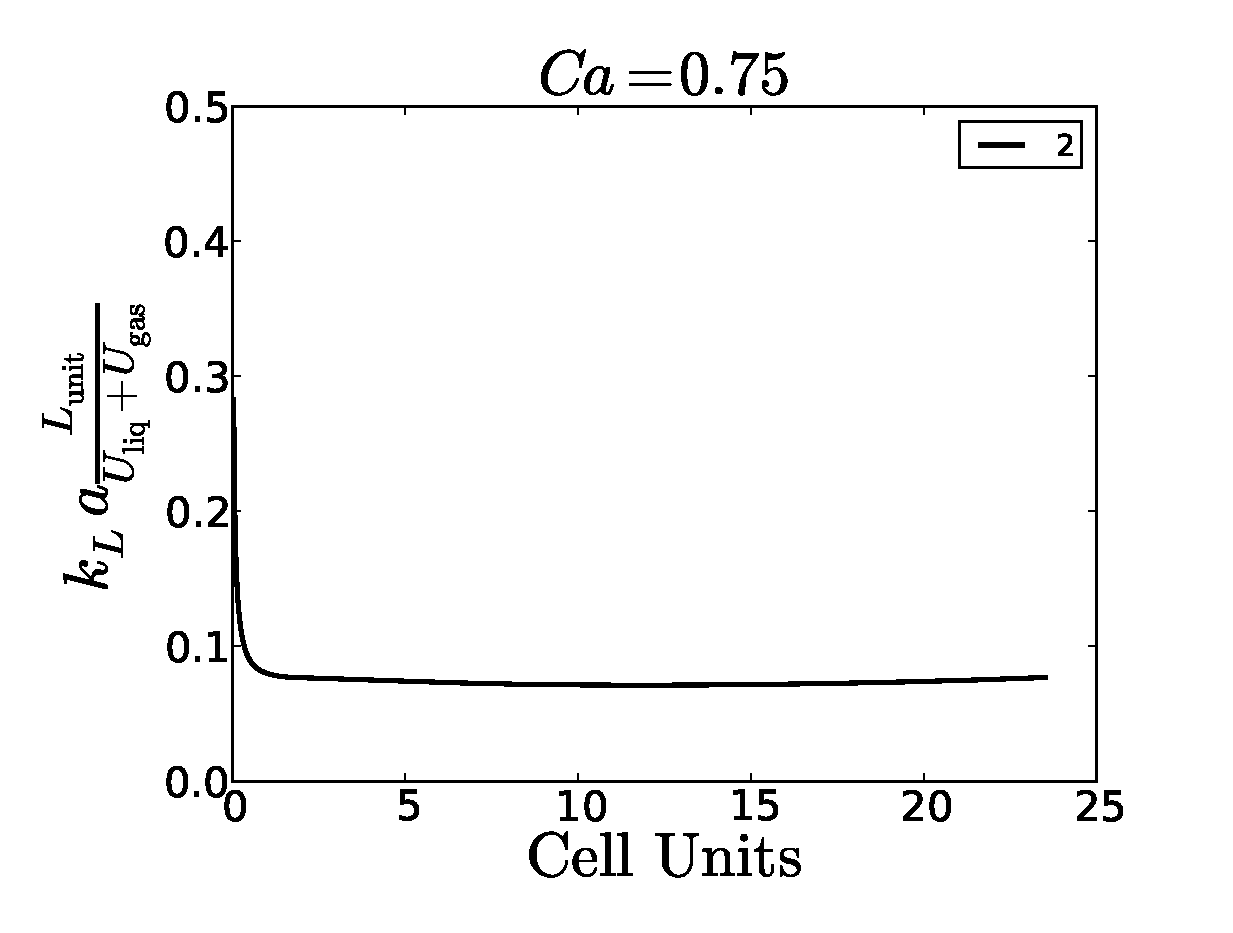
\includegraphics[width=0.5\textwidth]{Figures/aver_conc_scale_ca05.eps}
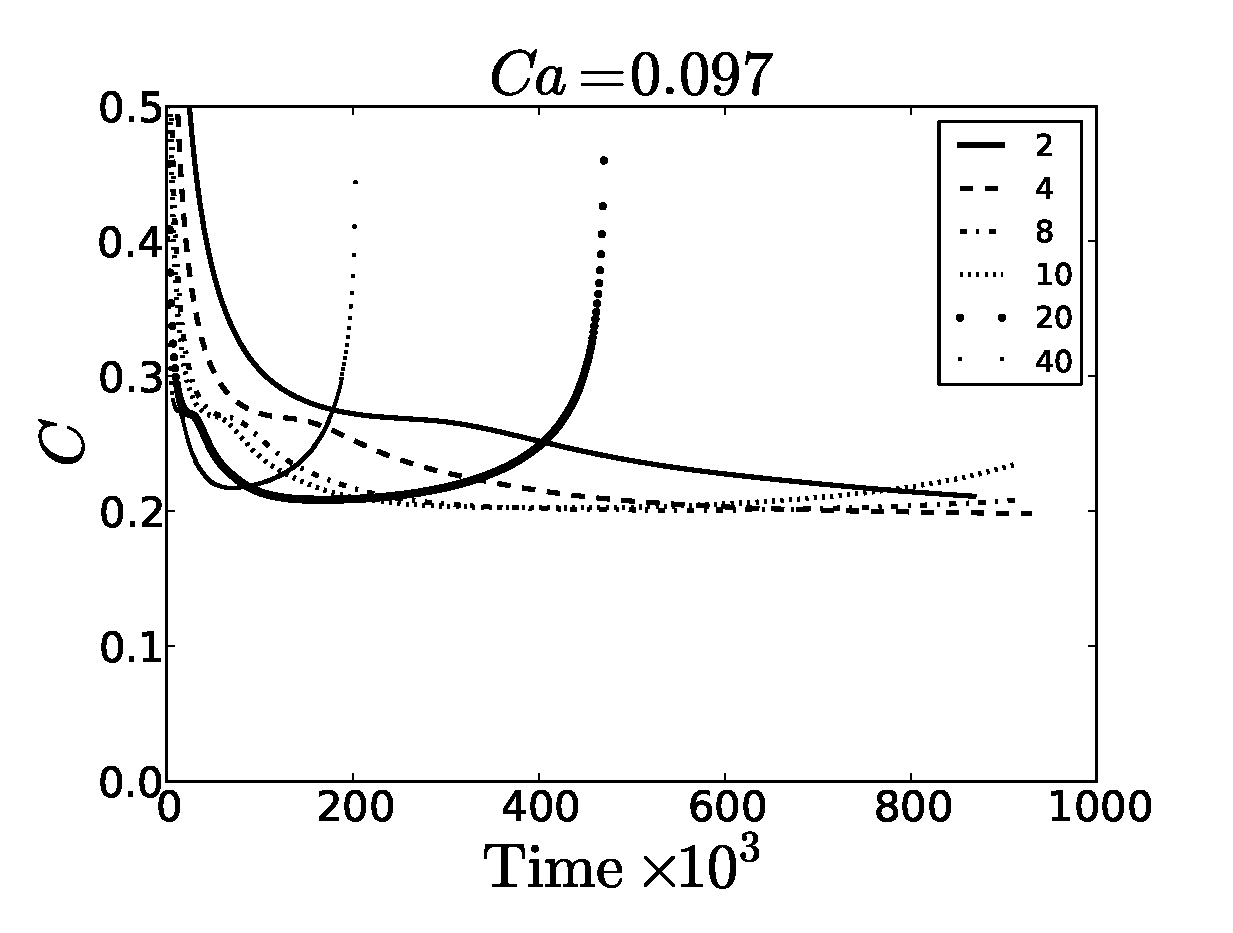
\includegraphics[width=0.5\textwidth]{Figures/aver_conc_scale_ca097.eps}\\
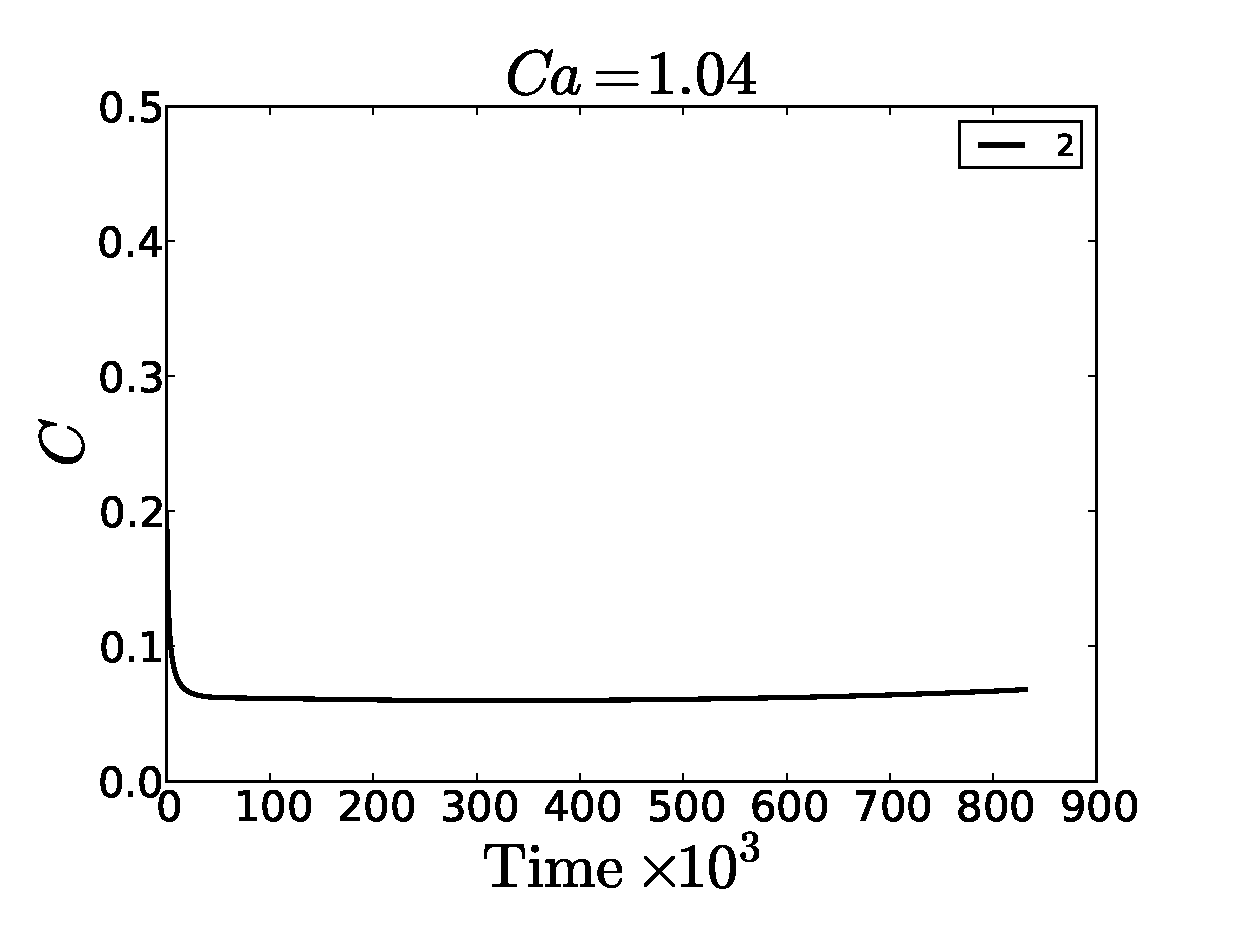
\includegraphics[width=0.5\textwidth]{Figures/aver_conc_scale_ca14.eps}\\
\caption{Volumetric mass transfer coefficient for different capillaries and scales. One can see the
excellent agreement. \label{fig:aver:conc:different:capillaries}}
\end{figure}
One of interesting correlations for the mass transfer volumetric coefficient was presented by
\citet{yue-mass}:
\beqal
&\vol=\frac{2}{d_h}\Bigl(\frac{D \ububble}{\lbubble+\lslug}\Bigr)^{0.5}
\Bigl(\frac{\lbubble}{\lbubble+\lslug}\Bigr)^{0.3}\\
&\vol \frac{\lunit}{\ugas+\uliq}=2\frac{\lunit}{d_h} \Bigl(\frac{D 
}{\lunit (\ububble+\ugas)} \frac{\ububble}{\ugas+\uliq}\Bigr)^{0.5}
\Bigl(\frac{\lbubble}{\lbubble+\lslug}\Bigr)^{0.3} \propto Pe^{-\frac{1}{2}}\\
&\vol \frac{\lunit}{\ugas+\uliq}=2\frac{\lunit}{d_h} \Bigl(\frac{D 
}{\lunit (\ububble+\ugas)} \frac{\ububble}{\ugas+\uliq}\Bigr)^{0.5}
\Bigl(\frac{\lbubble}{\lbubble+\lslug}\Bigr)^{0.3} \propto Pe^{-\frac{1}{2}}
\feqal
\begin{figure}
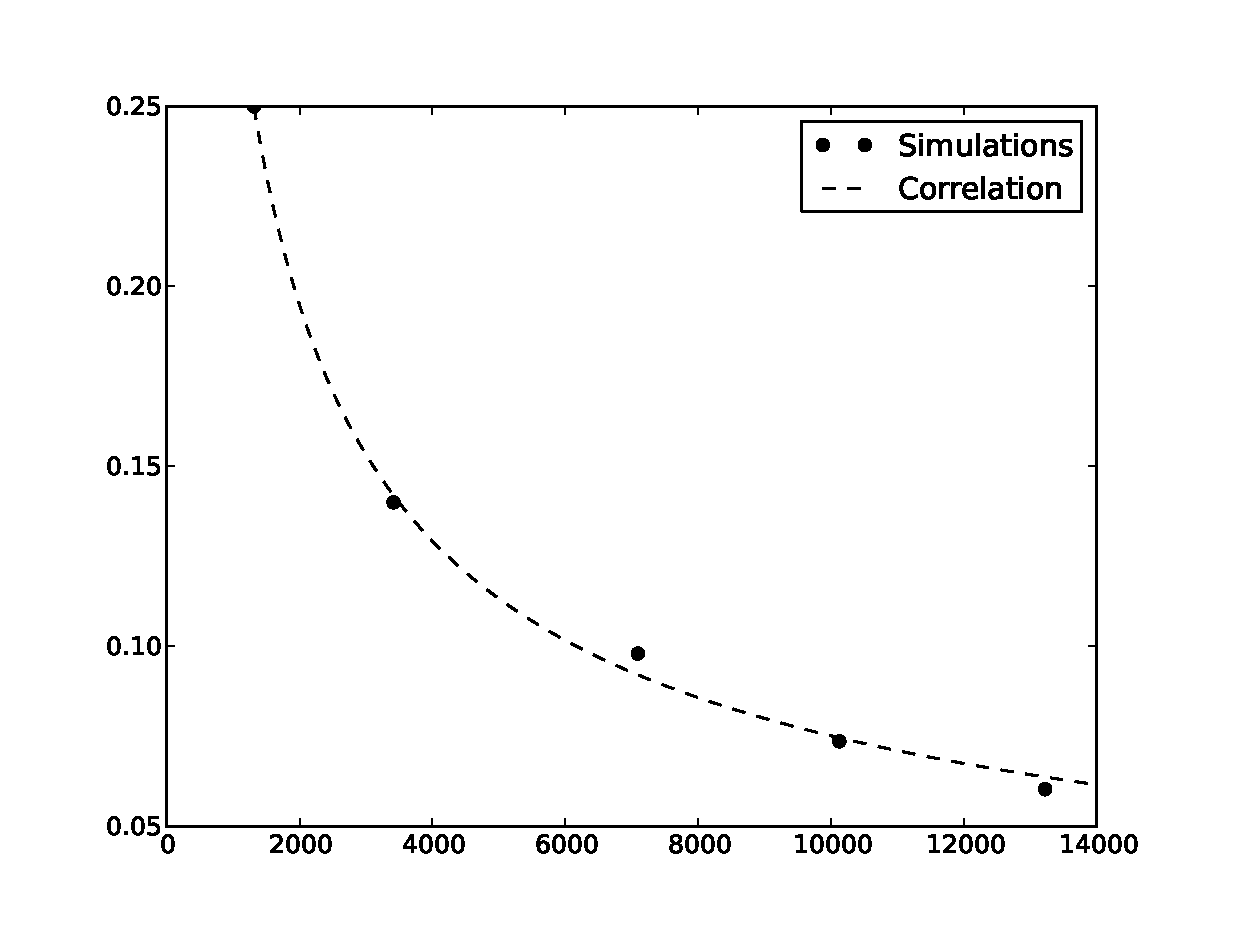
\includegraphics[width=\textwidth]{Figures/volumetric_mass_peclet.eps}
\end{figure}

\section{Real calculations}
This section examines different cells for the capillary $Ca=0.097$. The coefficient is
non-dimensionalized in the following manner $\vol \frac{\lunit}{\ugas+\uliq}$. Therefore, we
examined the average concentrations in different units and for different scalings. Therefore the
average concentration between two different cells have to be of the following value:
\beqal
&C_1=C(x)=C^* \Bigl(1-e^{-\vol \frac{x}{\ugas+\uliq}}\Bigr)\\
&C_2=C(x+L)=C^* \Bigl(1-e^{-\vol \frac{x+L}{\ugas+\uliq}}\Bigr)\\
k_L\frac{L}{\ugas+\uliq}=\frac{C^*-C_1}{C^{*}-C_2}
\feqal
One can see that this number is different in comparison with the number used for periodic boundary
conditions. Thus, the domain transformation from time domain to the coordinate domain is not
straightforward and require other definitions. For example by definition we took $C_1$ and $C_2$ to
be average concentrations over different units. One can see Fig. \ref{fig:unit:8} for
average coefficients and corresponding volumetric mass transfer coefficients.
\subsection{4 units}
\begin{figure}[htb!]
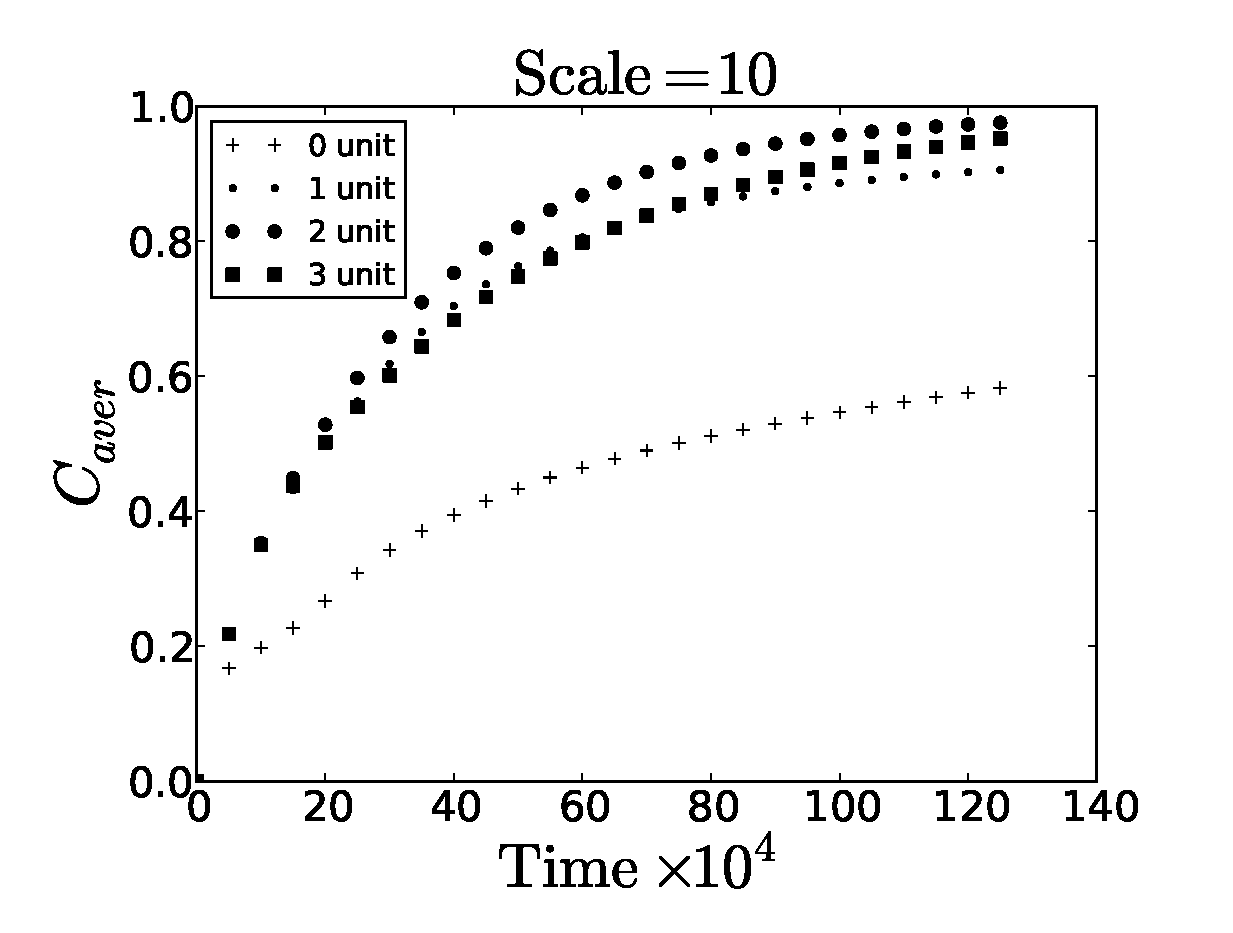
\includegraphics[width=0.5\textwidth]{Figures/aver_units4scale10.eps}\hfill
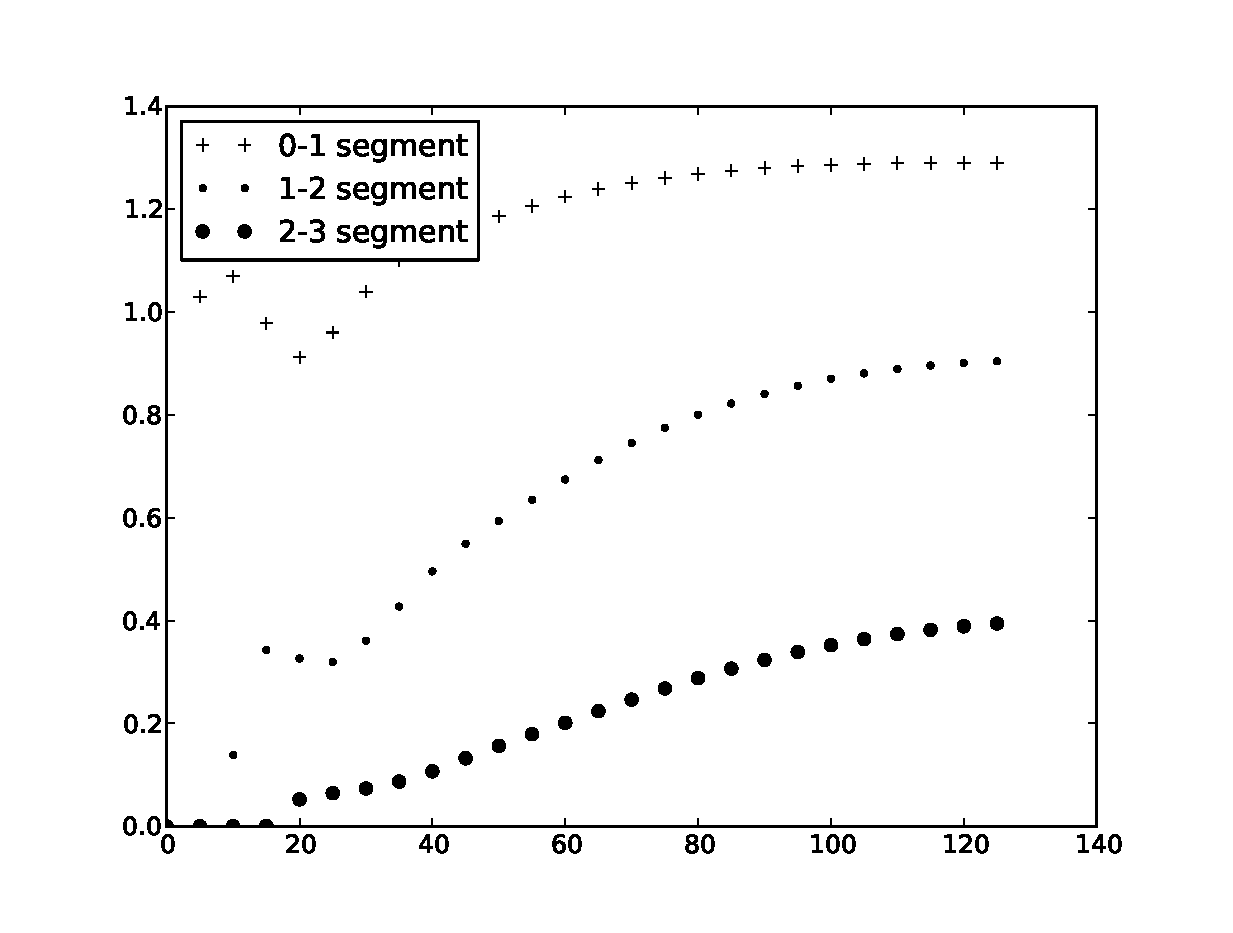
\includegraphics[width=0.5\textwidth]{Figures/coeff_units4scale10.eps}\\
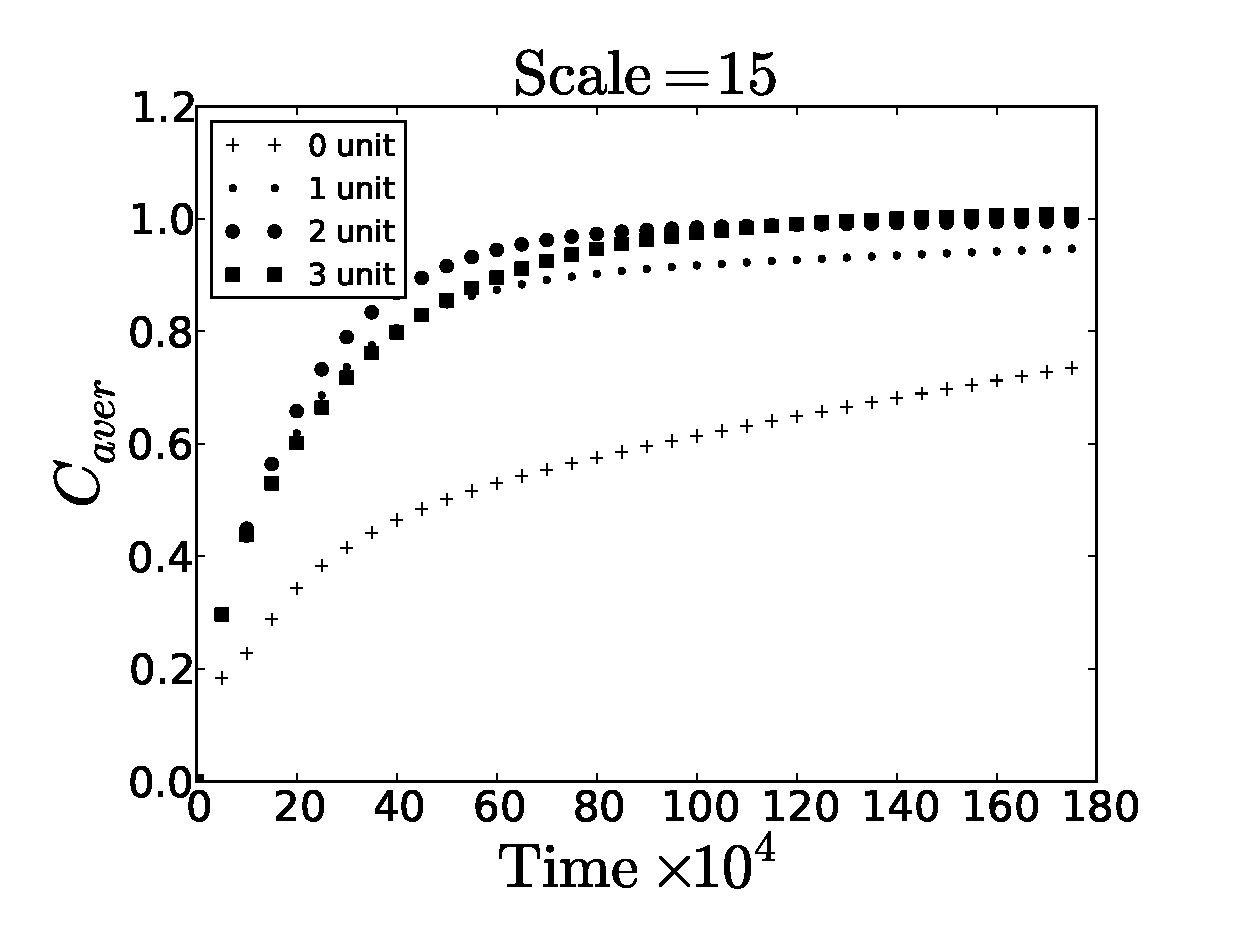
\includegraphics[width=0.5\textwidth]{Figures/aver_units4scale15.eps}\hfill
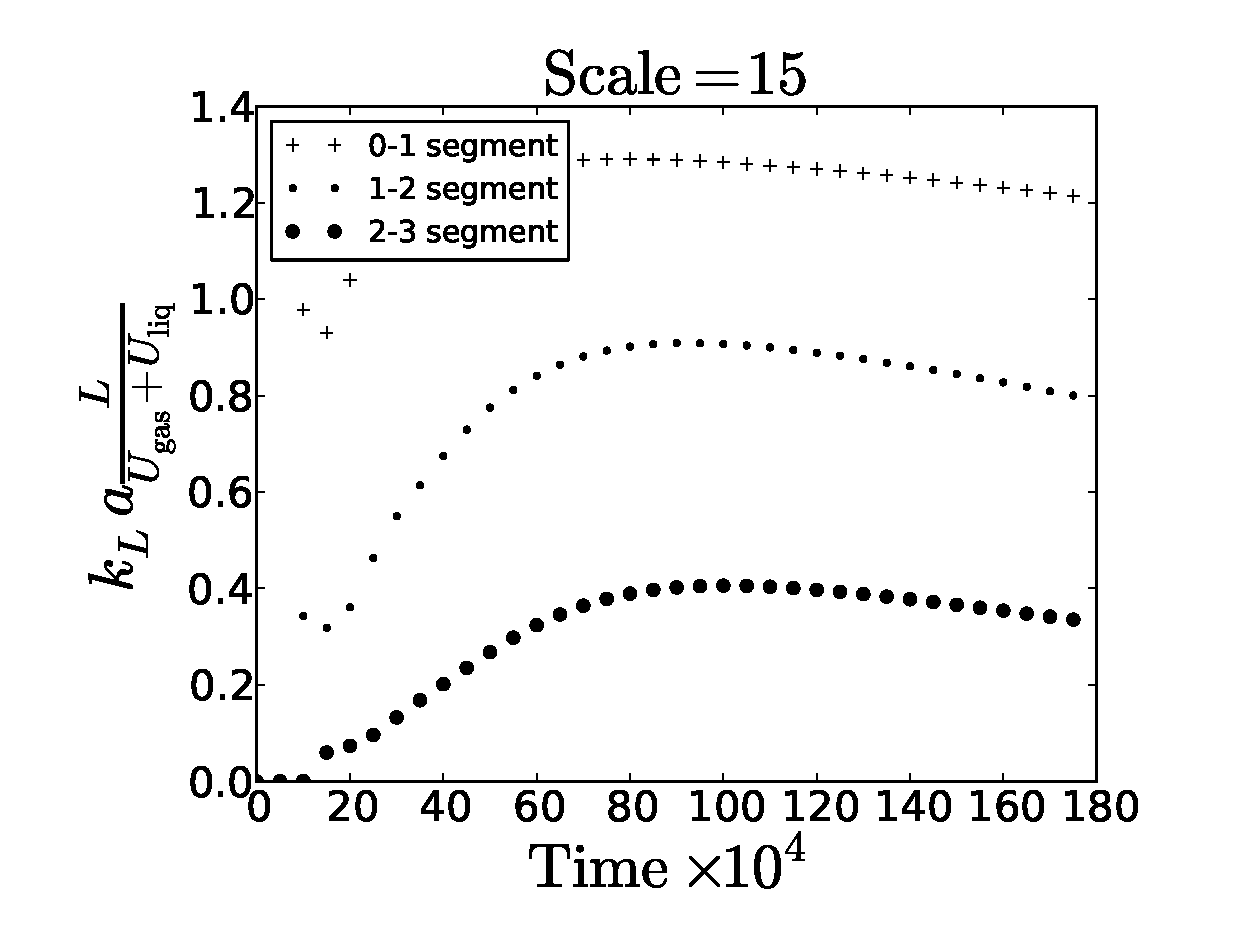
\includegraphics[width=0.5\textwidth]{Figures/coeff_units4scale15.eps}\\
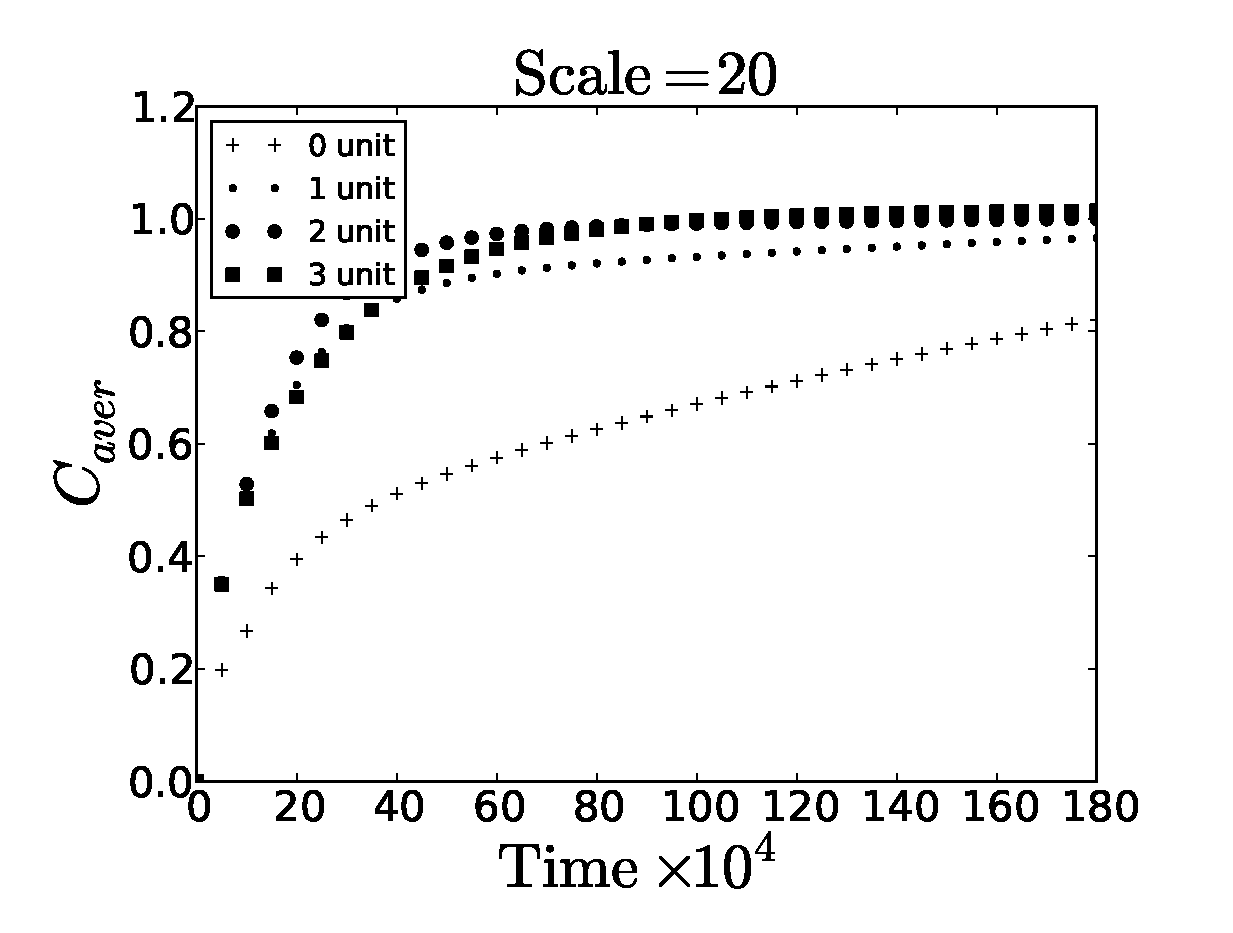
\includegraphics[width=0.5\textwidth]{Figures/aver_units4scale20.eps}\hfill
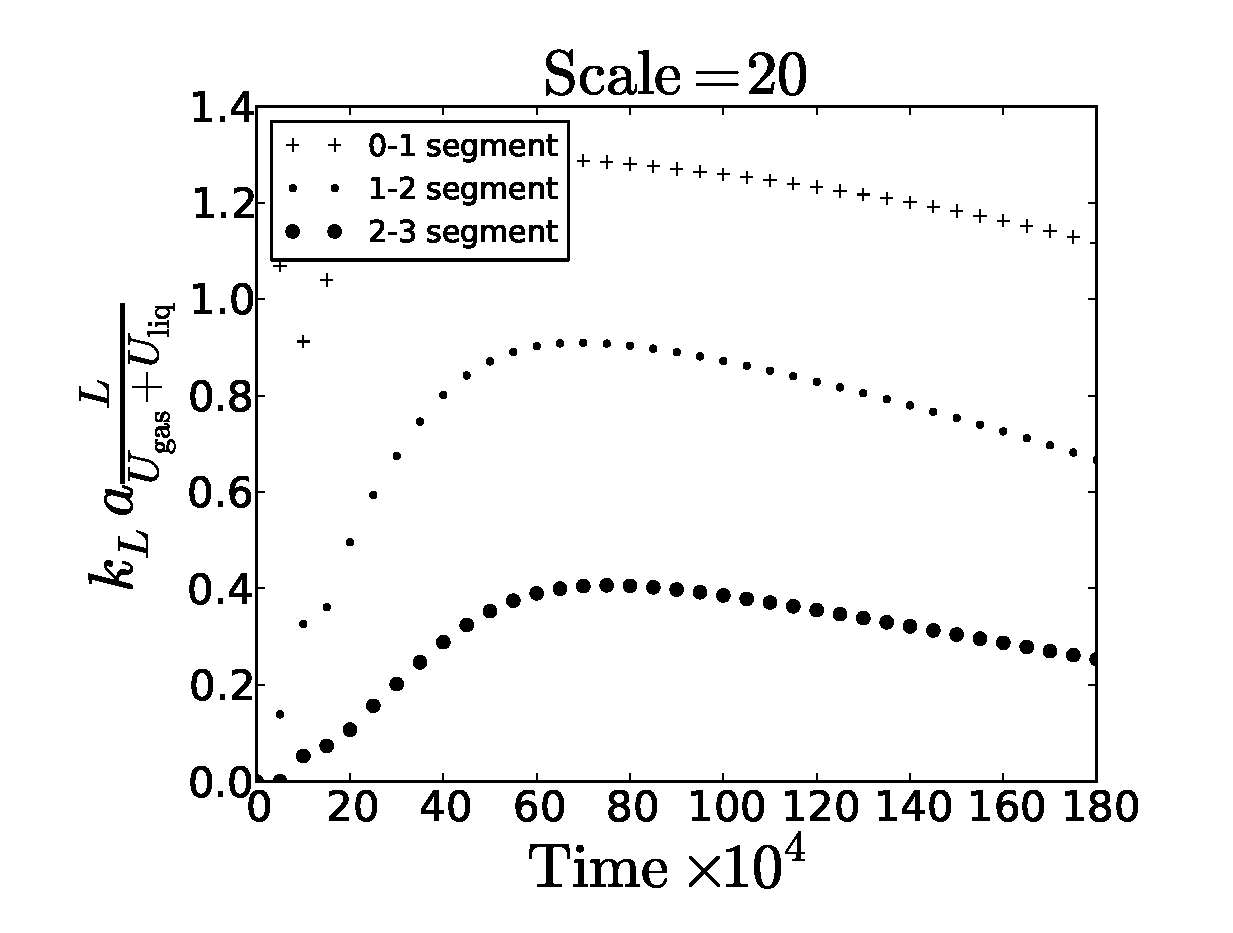
\includegraphics[width=0.5\textwidth]{Figures/coeff_units4scale20.eps}\\
\caption{Average concentrations and volumetric coefficients for $4$ units.
\label{fig:unit:4}}
\end{figure}
The more interesting picture is actually moving window average which is calculated as:
\beq
\label{moving:average}
\vol\frac{\lunit}{\ugas+\uliq}=\frac{\lunit}{\ububble (t_2
-t_1)}\ln\Bigl(\frac{C^*-C_1}{C^*-C_2}\Bigr)
\feq
One can see those moving averages in Fig. \ref{window4}.
\begin{figure}[htb!]
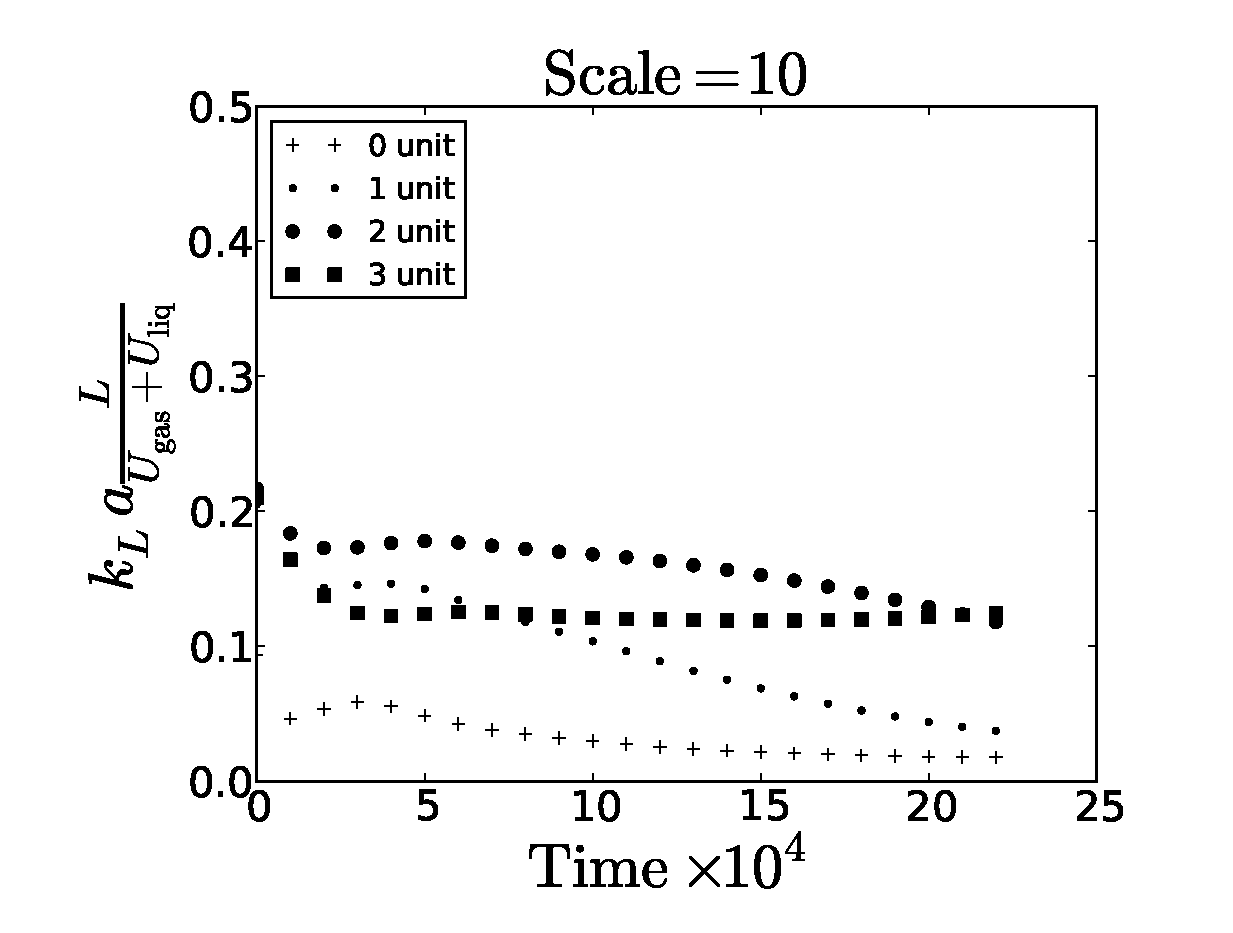
\includegraphics[width=0.7\textwidth]{Figures/aver_moving_window4scale10.eps}\\
\includegraphics[width=0.7\textwidth]{Figures/aver_moving_window4scale15.eps}\\
\includegraphics[width=0.7\textwidth]{Figures/aver_moving_window4scale20.eps}\\
\caption{Moving averages defined in Eq. \ref{moving:average} for 4 units
\label{fig:moving:average:window4}}
\end{figure}

\subsection{6 units} 
\begin{figure}[htb!]
\includegraphics[width=0.5\textwidth]{Figures/aver_units6scale10.eps}\hfill
\includegraphics[width=0.5\textwidth]{Figures/coeff_units6scale10.eps}\\
\includegraphics[width=0.5\textwidth]{Figures/aver_units6scale15.eps}\hfill
\includegraphics[width=0.5\textwidth]{Figures/coeff_units6scale15.eps}\\
\includegraphics[width=0.5\textwidth]{Figures/aver_units6scale20.eps}\hfill
\includegraphics[width=0.5\textwidth]{Figures/coeff_units6scale20.eps}\\
\caption{Average concentrations and volumetric coefficients for $8$ units.
\label{fig:unit:10}}
\end{figure}

Another moving concentrations window is presented in Fig. \ref{fig:moving:average:window6}.
\begin{figure}[htb!]
\includegraphics[width=0.7\textwidth]{Figures/aver_moving_window6scale10.eps}\\
\includegraphics[width=0.7\textwidth]{Figures/aver_moving_window6scale15.eps}\\
\includegraphics[width=0.7\textwidth]{Figures/aver_moving_window6scale20.eps}\\
\caption{Moving averages defined in Eq. \ref{moving:average} for $8$ units.
\label{fig:moving:average:window6}}
\end{figure}



\subsection{8 units} 
\begin{figure}[htb!]
\includegraphics[width=0.5\textwidth]{Figures/aver_units8scale10.eps}\hfill
\includegraphics[width=0.5\textwidth]{Figures/coeff_units8scale10.eps}\\
\includegraphics[width=0.5\textwidth]{Figures/aver_units8scale15.eps}\hfill
\includegraphics[width=0.5\textwidth]{Figures/coeff_units8scale15.eps}\\
\includegraphics[width=0.5\textwidth]{Figures/aver_units8scale20.eps}\hfill
\includegraphics[width=0.5\textwidth]{Figures/coeff_units8scale20.eps}\\
\caption{Average concentrations and volumetric coefficients for $8$ units.
\label{fig:unit:8}}
\end{figure}

Another moving concentrations window is presented in Fig. \ref{fig:moving:average:window8}.
\begin{figure}[htb!]
\includegraphics[width=0.7\textwidth]{Figures/aver_moving_window8scale10.eps}\\
\includegraphics[width=0.7\textwidth]{Figures/aver_moving_window8scale15.eps}\\
\includegraphics[width=0.7\textwidth]{Figures/aver_moving_window8scale20.eps}\\
\caption{Moving averages defined in Eq. \ref{moving:average} for $8$ units.
\label{fig:moving:average:window8}}
\end{figure}


\subsection{10 units} 
\begin{figure}[htb!]
\includegraphics[width=0.5\textwidth]{Figures/aver_units10scale10.eps}\hfill
\includegraphics[width=0.5\textwidth]{Figures/coeff_units10scale10.eps}\\
\includegraphics[width=0.5\textwidth]{Figures/aver_units10scale15.eps}\hfill
\includegraphics[width=0.5\textwidth]{Figures/coeff_units10scale15.eps}\\
\includegraphics[width=0.5\textwidth]{Figures/aver_units10scale20.eps}\hfill
\includegraphics[width=0.5\textwidth]{Figures/coeff_units10scale20.eps}\\
\caption{Average concentrations and volumetric coefficients for $8$ units.
\label{fig:unit:10}}
\end{figure}

Another moving concentrations window is presented in Fig. \ref{fig:moving:average:window10}.
\begin{figure}[htb!]
\includegraphics[width=0.7\textwidth]{Figures/aver_moving_window10scale10.eps}\\
\includegraphics[width=0.7\textwidth]{Figures/aver_moving_window10scale15.eps}\\
\includegraphics[width=0.7\textwidth]{Figures/aver_moving_window10scale20.eps}\\
\caption{Moving averages defined in Eq. \ref{moving:average} for $8$ units.
\label{fig:moving:average:window10}}
\end{figure}

\section{Open boundary conditions}
\begin{figure}
\includegraphics[width=0.5\textwidth]{Figures/jos_aver_conc_scale_ca0097.eps}
\includegraphics[width=0.5\textwidth]{Figures/jos_aver_moving_window_ca0097.eps}\\
\includegraphics[width=0.5\textwidth]{Figures/jos_aver_conc_scale_ca0254.eps}
\includegraphics[width=0.5\textwidth]{Figures/jos_aver_moving_window_ca0254.eps}\\
\caption{Open boundary conditions. \label{fig:open:boundary:jos}}
\end{figure}

\section{Symmetric boundary conditions}
\begin{figure}
\includegraphics[width=0.5\textwidth]{Figures/sym_aver_conc_scale_ca0097.eps}
\includegraphics[width=0.5\textwidth]{Figures/sym_aver_moving_window_ca0097.eps}\\
\includegraphics[width=0.5\textwidth]{Figures/sym_aver_conc_scale_ca0254.eps}
\includegraphics[width=0.5\textwidth]{Figures/sym_aver_moving_window_ca0254.eps}\\
\caption{Symmetric boundary conditions. \label{fig:open:boundary:sym}}
\end{figure}


\appendix
\section{Analytical solution for parabolic profile with zero velocity gradient at $0$}
The problem is defined in terms of PDE as follows: 
\beq
\label{diffusion:zero:gradient:start}
\begin{aligned}
&\frac{\partial C}{\partial x} U(y)=D\frac{\partial^2 C}{\partial y^2}\\
&C(0,y)=C_0,\, C(x,0)=C_{wall},\, \frac{\partial C}{\partial y }(x,\delta)=0\\
&U(y)=U_0 \Bigl(\frac{y}{\delta}\Bigr)^2
\end{aligned}
\feq
The non-dimensional parameters are introduced:
\beq
\begin{aligned}
&\frac{\partial C}{\partial \frac{x}{H}} \frac{U_0}{H}
\Bigl(\frac{y}{H}\Bigr)^2=\frac{D}{H^2}\frac{\partial^2 C}{\partial \frac{y^2}{H^2}}\\
&C(0,y)=C_0,\, C(x,0)=C_{wall},\, \frac{\partial C}{\partial y }(x,H)=0\\
\end{aligned}
\feq
After a change of variables:
\beq
\begin{aligned}
&\zeta=\frac{x}{H} \frac{D}{U_0 H}=\frac{1}{Pe}\frac{x}{H}\\
&\xi=\frac{y}{H}
\end{aligned}
\feq
, Eq. \ref{diffusion:zero:gradient:start} with boundary conditions becomes as follows:
\beq
\label{diffusion:zero:gradient:middle}
\begin{aligned}
&\frac{\partial C}{\partial \zeta}\xi^2=\frac{\partial^2 C}{\partial \xi^2}\\
&C(0,\xi)=C_0\\
&C(\zeta,0)=C_{wall}\\
&\frac{\partial C}{\partial \xi}(\zeta,1)=0\\
\end{aligned}
\feq 
Still Eq. \ref{diffusion:zero:gradient:middle} cannot be solved with the separation of variables as it requires homogenous
boundary conditions. Thus, let us introduce the new variable, $\Theta=C-C_{wall}$, which makes the system to be with homogenous boundary conditions:
\beq
\begin{aligned}
&\frac{\partial \Theta}{\partial \zeta}=\frac{1}{\xi^2}\frac{\partial^2 \Theta}{\partial \xi^2}\\
&\Theta(0,\xi)=C_0-C_{wall}\\
&\Theta(\zeta,0)=0,\, \partial_{\xi}\Theta(\zeta,1)=0\\
\end{aligned}
\feq 
This equation can be solved by separation of variables if the solutions is represented as the
multiplication of two functions $\Theta(\zeta,\xi)=X(\zeta)Y(\xi)$:
\beq
\begin{aligned}
&\frac{\mathrm{d} X(\zeta)}{\mathrm{d} \zeta}Y(\xi)=\frac{X(\zeta)}{\xi^2}\frac{\mathrm{d^2}
Y(\xi)}{\mathrm{d}\xi^2}\\
&\frac{1}{X(\zeta)}\frac{\mathrm{d} X(\zeta)}{\mathrm{d} \zeta}=\frac{1}{\xi^{2} Y(\xi)}
\frac{\mathrm{d^2} Y(\xi)}{\mathrm{d}\xi^2}
\end{aligned}
\feq
The left and right parts depend on different variables. Therefore to be equal to each other both
parts shall equal to constant, say $-m^4$. Thus, the separation of the variables leads to two ODEs:
\begin{equation*}
\begin{aligned}
&\frac{\mathrm{d}X(\zeta)}{\mathrm{d}\zeta}=-m^4 X(\zeta)\\
&\frac{\mathrm{d^2}Y(\xi)}{\mathrm{d}\xi^2}+m^4 \xi^2 Y(\xi)=0\\ 
\end{aligned}
\end{equation*}
The solution of the first equation is the exponential function:
\beq
X(\zeta)=\exp(-m^4 \zeta)\\
\feq
The solutions of the second equation are two hypergeometric function which can be expressed through
the Bessel functions \cite{abramowitz}:
\beq
\begin{aligned}
&Y_1=\sqrt{\xi}J_{\frac{1}{4}}\Bigl(\frac{m^2 \xi^2}{2}\Bigr)\\
&Y_2=\sqrt{\xi}J_{-\frac{1}{4}}\Bigl(\frac{m^2 \xi^2}{2}\Bigr)\\
&Y'_1=m^2 \xi^{3/2} J_{-\frac{3}{4}}\Bigl(\frac{m^2 \xi^2}{2}\Bigr)\\
&Y'_2=m^2 \xi^{3/2} J_{\frac{3}{4}}\Bigl(\frac{m^2 \xi^2}{2}\Bigr)\\
\end{aligned}
\feq
The solution is the summation of two functions:
\begin{equation*}
Y(x)=C_1 Y_1(x)+C_2 Y_2(x). 
\end{equation*}
One can find coefficients from the boundary conditions:
\beq
\begin{aligned}
&Y(0)=0=C_1 Y_1(0)+C_2 Y_2(0)\\
&Y_1(0)=0,\,Y_2(0)=\frac{\sqrt{2}}{\sqrt{m} \Gamma(3/4)}\, C_2=0\\
&Y'(1)=0=C_1 Y'_1(1)+C_2 Y'_2(1)=C_1 Y'_1(1)\\
&J_{-\frac{3}{4}}\Bigl(\frac{m^2}{2}\Bigr)=0
\end{aligned}
\feq
Therefore one needs to find zeros of $J_{-\frac{3}{4}}\Bigl(\frac{m^2}{2}\Bigr)$. To give some
numerical values:
$m_1=1.454997085$, $m_2=2.927133004$, $m_3=3.857578101$, $m_4=4.601777732$, $m_5=5.240824067$.
Therefore, the solution in a general form is represented as:
\beq
\Theta(\zeta,\xi)=\sum_m{C_m \sqrt{\xi} J_{\frac{1}{4}}\Bigl(\frac{m^2
\xi^2}{2}\Bigr)\exp(-m^4 \zeta)}
\feq
To find unknown coefficients $C_m$ one needs to substitute the expression above to the initial
condition:
\beq
\Theta(0,\xi)=C_0-C_{wall}=\sum_m{C_m \sqrt{\xi}J_{\frac{1}{4}}\Bigl(\frac{m^2
\xi^2}{2}\Bigr)}\\
\feq
Using the Stourm-Liouville theorem one can multiply by $\xi^{5/2}
J_{\frac{1}{4}}\Bigl(\frac{m^2 \xi^2}{2}\Bigr)$ and integrate left and right parts of the equation:
\beq
\begin{aligned}
&\bigl(C_0-C_{wall}\bigr) \int_{\xi=0}^{1}{\xi^{5/2} J_{\frac{1}{4}}\Bigl(\frac{m^2
\xi^2}{2}\Bigr)\mathrm{d}\xi}=C_m\int_{\xi=0}^{1}{\xi^3 J_{\frac{1}{4}}^2\Bigl(\frac{m^2
\xi^2}{2}\Bigr)\mathrm{d}\xi}\\
&C_m = (C_0-C_{wall}) \frac{\int_{\xi=0}^{1}{\xi^{5/2} J_{\frac{1}{4}}\Bigl(\frac{m^2
\xi^2}{2}\Bigr)\mathrm{d}\xi}}{\int_{\xi=0}^{1}{\xi^3 J_{\frac{1}{4}}^2\Bigl(\frac{m^2
\xi^2}{2}\Bigr)\mathrm{d}\xi}}
\end{aligned}
\feq
Therefore, the overall solution is specified as:
\beq
\begin{aligned}
&C(x,y)=C_{wall}+\sum_{m}{C_m
\sqrt{\frac{y}{H}}J_{\frac{1}{4}}\Bigl(\frac{m^2}{2}\frac{y^2}{H^2}\Bigr)\exp\Bigl(-\frac{m^4}{Pe}
\frac { x }{H}\Bigr)}\\
&C_m = (C_0-C_{wall}) \frac{\int_{\xi=0}^{1}{\xi^{5/2} J_{\frac{1}{4}}\Bigl(\frac{m^2
\xi^2}{2}\Bigr)\mathrm{d}\xi}}{\int_{\xi=0}^{1}{\xi^3 J_{\frac{1}{4}}^2\Bigl(\frac{m^2
\xi^2}{2}\Bigr)\mathrm{d}\xi}}
\end{aligned}
\feq
For the sake of completeness, we list $5$ first coefficients $C_1=-1.5217$, $C_2=-0.4933$, $C_3=-0.3243$, $C_4=-0.2486$, $C_5=-0.2044$. 
\subsection{The parabolic profile mass transfer and comparison}
The problem we want to address can be formulated through the following PDE:
\beq
\begin{aligned}
&\frac{\partial C}{\partial x} U(y)=D\frac{\partial^2 C}{\partial y^2}\\
&C(0,y)=0,\, C(x,\pm \delta)=C_s,\, \frac{\partial C}{\partial y }(x,0)=0\\
&U(y)=U_0 \Bigl(1-\bigl(\frac{y}{\delta}\bigr)^2\Bigr)
\end{aligned}
\feq
The same procedure can be done as in the previous case to redefine variables. After substitution
the following can be obtained:
\beq
\begin{aligned}
&\frac{\partial \Theta}{\partial \zeta}(1-\xi^2)=\frac{\partial^2 C}{\partial \xi^2}\\
\Theta(\zeta,\xi)=C-C_s\,\Theta(0,\xi)=-C_s\,\Theta(0,\pm 1)=0\\
\end{aligned}
\feq
After separation of variables, $\Theta(\zeta,\xi)=X(\zeta)Y(\xi)$ one can come up with two
equations:
\beq
\label{fourier:separation:variables}
\begin{aligned}
&\frac{\mathrm{d}X(\zeta)}{\mathrm{d}\zeta}+m^4 X(\zeta)=0\\
&\frac{\mathrm{d^2}Y(\xi)}{\mathrm{d}\xi^2}+m^4 (1-\xi^2) Y(\xi)=0
\end{aligned}
\feq
The first equation has a solution:
\beq
X(\zeta)=\exp(-m^4 \zeta)
\feq
The second equation can be simplified after substitution $\bar{\xi}=m \sqrt{2} \xi$ to the standard
equation:
\beq
Y''-\Bigl(\frac{1}{4}\xi^2+a\Bigr)Y=0.
\feq
The equation above has two solutions via parabolic cylinder functions or through the confluent
hypergeometric function \cite{abramowitz}:
\beq
\begin{aligned}
&Y_1=e^{-x^2/4} {_1F_1}\Bigl(\frac{a}{2}+\frac{1}{4},\frac{1}{2},\frac{x^2}{2}\Bigr)\\
&Y_2=e^{-x^2/4} {_1F_1}\Bigl(\frac{a}{2}+\frac{3}{4},\frac{3}{2},\frac{x^2}{2}\Bigr)\\
\end{aligned}
\feq 
Taking symmetry conditions in the consideration by leaving only even solution, Eq.
(\ref{fourier:separation:variables}) has a solution as:
\beq
Y_m=C_m e^{-m^2 x^2/2} {_1F_1}\Bigl(-\frac{m^2}{4}+\frac{1}{4},\frac{1}{2},m^2 x^2\Bigr) 
\feq
To satisfy boundary condition we need to find zeros of the hypergeometric function, i.e.
${_1F_1}\Bigl(-\frac{m^2}{4}+\frac{1}{4},\frac{1}{2},m^2 \Bigr)=0$. First ten eigenvalues can be
found using numerical methods, as $1.2967$, $2.3811$,$3.1093$,$3.6969$,$4.2032$,$4.6548$,$5.0662$,
$5.4467$, $5.8023$,$6.1373$. One needs to satisfy one more condition to obtain coefficients $C_m$:
\beq
-C_{s}=\sum_m{C_m e^{-m^2 x^2/2} {_1F_1}\Bigl(-\frac{m^2}{4}+\frac{1}{4},\frac{1}{2},m^2
x^2\Bigr)} 
\feq
One can multiply both parts on $(1-x^2){_1F_1}\Bigl(-\frac{m^2}{4}+\frac{1}{4},\frac{1}{2},m^2
x^2\Bigr)$ and through orthoganality Sturm-Liouiville theorem obtain coefficients:
\beq
\label{coeff:series:parabolic:profile}
C_m=-C_s \frac{\int_{x=0}^{1}{(1-x^2)e^{-m^2 x^2/2}
{_1F_1}\Bigl(-\frac{m^2}{4}+\frac{1}{4},\frac{1}{2},m^2
x^2\Bigr)\mathrm{d}x}}{\int_{x=0}^{1}{(1-x^2)e^{-m^2 x^2/2}
{_1F_1}\Bigl(-\frac{m^2}{4}+\frac{1}{4},\frac{1}{2},m^2
x^2\Bigr)^2\mathrm{d}x}}
\feq
Therefore a whole solution can be written as:
\begin{equation}
C=C_{s}-C_s \sum_{m=0}{C_m e^{-m^4 \frac{x}{\delta}\frac{1}{Pe}} e^{-m^2
y^2/(2\delta^2)}{_1F_1}\Bigl(-\frac{m^2}{4}+\frac{1}{4},\frac{1}{2},m^2 \frac{y^2}{\delta^2}\Bigr)},
\end{equation}
where coefficients $C_m$ are taken from Eq. (\ref{coeff:series:parabolic:profile}). The comparison
between profiles is represented in Fig. \ref{fig:parabolic:comparison}.
\begin{figure}[htb!]
\includegraphics[width=\textwidth]{Figures/parabolic_profile_comparison.eps}
\caption{Comparison between analytical profile and simulations with pressure antibounceback
conditions. One can see given a low resolution of the profile a nice coincedence.}
\end{figure}

\section{Free surface boundary conditions}
\label{appendix-free-surface}
There are a few implementations of free boundary conditions \cite{ginzburg-free,verberg-free}.
However, we developed the easy solver to impose the free surface boundary conditions at the
complicated surface of the bubble. The reason is to impose the symmetric boundary conditions.
Because the boundary is the staircase approximation, one can find the normal to the boundary which
is always located by the angle of multiple of $45$, see Fig. \ref{fig:free:surface}. Imposing the
symmetric boundary conditions requires $U_{n,F}$=$U_{n,B}$ and $U_{\tau,F}=U_{\tau,B}$. We can copy
populations in the certain order to do it, for example $f_{B,i}=f_{F,\bar{i}}$, where $c_i$ and
$c_{\bar{i}}$ are complementary directions, where $c_{i,n}=-c_{\bar{i},n}$ and
$c_{i,\tau}=c_{\bar{i},\tau}$, where $c_{i,n}=(\bm{c_i} \cdot \bm{n})\bm{n}$ and
$c_{i,\tau}=\bm{c_i}-(\bm{c_i}\cdot \bm{n})\bm{n}$.  

\begin{figure}
\includegraphics[width=\textwidth]{Figures/free_surface.eps}
\caption{Free-surface boundary condition represented in the lattice Boltzmann. By crosses we outline boundary nodes, by circle the fluid node is outlined. \label{fig:free:surface}}
\end{figure}
\bibliographystyle{unsrtnat}
\bibliography{paper}

\end{document}

